\documentclass[11pt,twoside,openright]{book}
\usepackage[paperwidth=170mm,paperheight=240mm,top=20mm,total={130mm,195mm}]{geometry}
% Reccomendations for thesis printing:
% - Write in (a) A4, (b) 170x240 mm.
% - Minimum margin of 2 cm on top and sides, 2.5 on bottom. Page numbers underneath margin. (Is this for a or b?) latex A4 does well above this automatically.
% - Fontsize: (a) 12, (b) 11
% - Numbering: Bottom centered or side aliged (right align odd, left align even numbers)
% - Chapters, table of contents, foreword etc on odd (right) pages.

% Force bibliography to appear in table of contents
\usepackage[nottoc]{tocbibind}

%For the title page pdf
\usepackage{pdfpages}

% For fancy quote
\usepackage{epigraph}

% For units
\usepackage{siunitx}

% Fancy chapter headings
\usepackage{titlesec, color}
\definecolor{gray75}{gray}{0.75}
\newcommand{\hsp}{\hspace{20pt}}
\titleformat{\chapter}[hang]{\Huge\bfseries}{\thechapter\hsp\textcolor{gray75}{|}\hsp}{0pt}{\Huge\bfseries}


% For norwegian characters (fontenc also needed for fancy chapter headings).
\usepackage[utf8]{inputenc}
\usepackage[T1]{fontenc}

\usepackage{comment}

% urls
\usepackage[hidelinks]{hyperref}

% Math
\usepackage{amsmath,bm,amssymb}

% Subfigures etc
\usepackage{graphicx,subcaption}

\usepackage{dirtytalk}

% Reference management
\newcommand{\Eqref}[1]{Eq.~\eqref{#1}}
\newcommand{\Eqsref}[1]{Eqs.~\eqref{#1}}
\newcommand{\Figref}[1]{Fig.~\ref{#1}}
\newcommand{\Figsref}[1]{Figs.~\ref{#1}}
\newcommand{\Secref}[1]{Sec.~\ref{#1}}
\newcommand{\Chapref}[1]{Chapter~\ref{#1}}


\newcommand{\first}{Paper I}

% Bibliography management
\usepackage[numbers,sort,compress]{natbib}
%\bibliographystyle{apsrev4-1}
\bibliographystyle{unsrtnat}


\begin{document}
\frontmatter
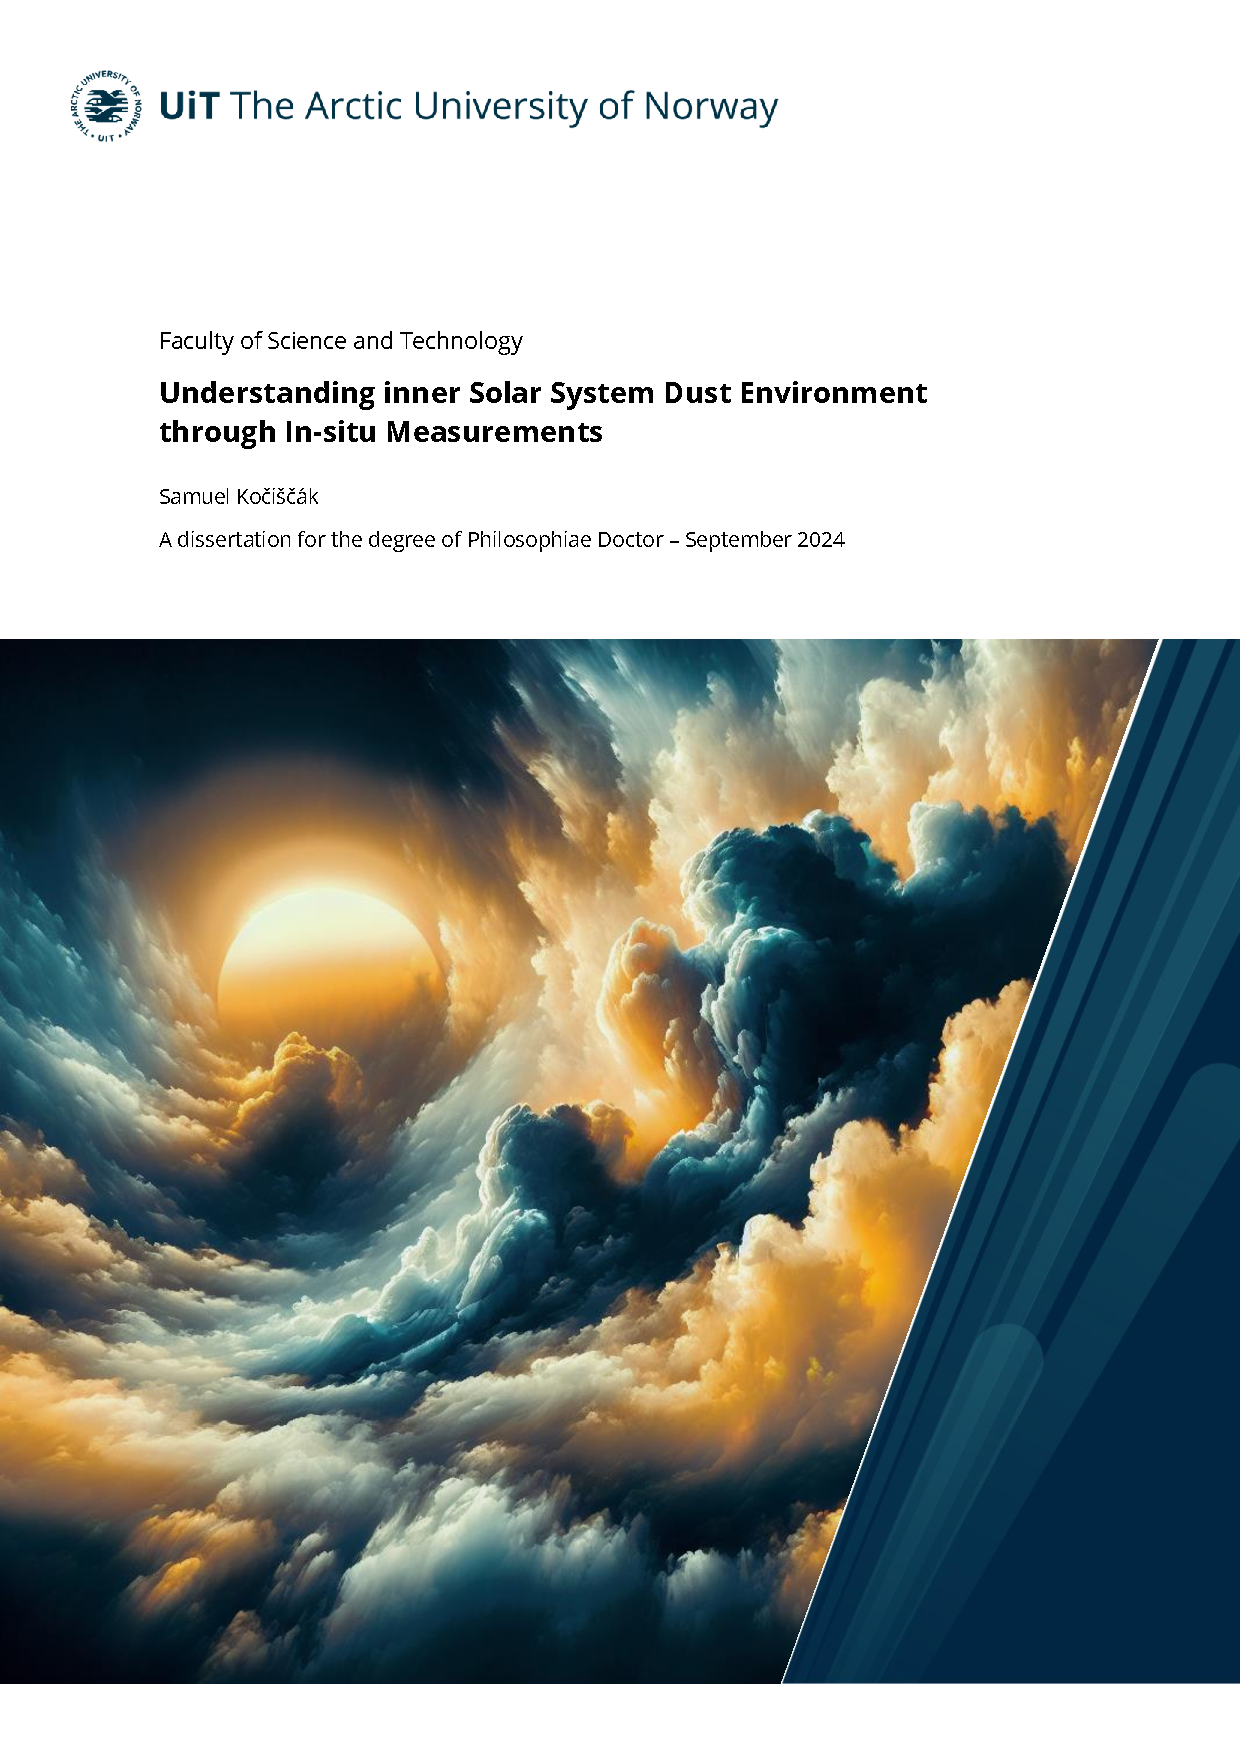
\includepdf{figures/PHD_first_page.pdf}

% To ensure: titlepage-blank-epigraph-blank-preface, with preface the first numbered page.
% We start counting from the first page, wiich is the epigraph.
\newpage\null\thispagestyle{empty}\newpage

\setcounter{page}{1}\thispagestyle{empty}\newpage
%\newpage\null\thispagestyle{empty}\newpage

\section*{Abstract}
many many science yo


\newpage\null\newpage
\section*{Acknowledgements}
Many thanks!
\newpage\null\newpage

\tableofcontents

\mainmatter

% Chapter: Intor
\chapter{Introduction}
\section{Plain language summary}

Rocky, icy, and metallic objects in space, smaller than asteroids, are called cosmic dust. Cosmic dust which originates in the solar system is called interplanetary dust, as opposed to cosmic dust which occupies the interstellar or intergalactic space. Cosmic dust is created as a debris of collisions of larger objects, but also by condensation of gaseous phase, or by being expelled from a larger body, such as a comet or a moon with active volcanism. It is responsible for the planetary rings, but also for the the zodiacal light observed in the post-sunset and the pre-sunrise night sky. The atmosphere of Earth offers a great target cosmic dust, and the cosmic dust entering the atmosphere is observable in the form of meteors. 

When spacecraft move through a dusty environment, they collide with dust grains in a random fashion. Little can be told about the dust cloud based on a single collision, but having observed many collisions, generalizations can be made about their size and speed distribution within the cloud. Even more can be told, if a theoretical framework for where the dost comes from and how it moves, is available. 

Cosmic dust is an integral part of the solar system, and its dynamics tells about the past and present of other bodies. For example, the structure of the rings of Saturn tells about the past evolution and the present sources of the saturnian dust. Similarly, the dust around the Sun is a probe into the vicinity of the Sun. By understanding how the circumsolar dust moves, where the collisions happen, where it is destroyed, and how its characteristics depend on its composition, we find more about the conditions around the Sun. 

We explore the measurements of two spacecraft: Solar Orbiter (SolO) and Parker Solar Probe (PSP). These are Sun-orbiting spacecraft, which use their electrical antennas to register collisions with dust grains. In order to understand the dynamics in the interplanetary dust cloud, we make use of their similarities and differences alike. Different statistical modeling approach must be taken to yield the maximum information in different regions, and in doing so, we find more about the dust grains' speed, masses, collisions, and location is space.

\section{Outline}

The aim of the thesis is to yield information on the interplanetary dust from electrical antenna measurements, using more mathematically precise approach than what was used previously, wherever possible. Single-grain dust properties, as well as forces acting on individual dust grains are introduced in Ch. \ref{ch:forces}. The dust grains in the Solar system compose the interplanetary dust cloud, in which grains of similar properties follow similar trajectories, forming individual dust populations, which are introduced in Ch. \ref{ch:populations}. To yield the most information possible, sharp statistical tools are needed, some of which are introduced in Ch. \ref{ch:statistics}. The dust detection principles are described in Ch. \ref{ch:detection}, where emphasis is put on antenna measurements. The articles, which make up a part of this thesis, are described in Ch. \ref{ch:sum-paper}. Finally, in Ch. \ref{ch:conclusion}, we conclude and offer outlook.

% Chapter: Dust forces
\chapter{Dust grain properties\\and~interactions}\label{ch:forces}
\chaptermark{Dust grain properties and interactions}
A dust grain in the Solar system is a subject to many interactions. Grains of different sizes and in different locations are naturally susceptible to be influenced by different forces. In this chapter, we describe the most important forces and interactions, their causes and effects, as well as their relevance for different dust grains. We will later use this to discuss the properties and dynamics of dust populations in the Solar system. 

\section{Characterizing a single grain}

Newton's second law of motion has it, that
\begin{equation}
\vec{a} = \frac{\vec{F}}{m},
\end{equation}
where $\vec{a}$ is the acceleration of the object with the mass $m$, induced by the net force $\vec{F}$. Mass of a dust grain is related to its volume $V$ and the mean density of $\rho$ as
\begin{equation}
    m = V \rho.
\end{equation}
The mean density depends on the composition and the structure of the grain. 

\subsubsection{Dust composition}

Dust grains are relatively hard to collect, and they are mostly collected in the atmosphere of or in the near vicinity of the Earth. Some collection methods, such as collection in antarctic ice or from the deep see sediments \citep{brownlee1985cosmic} and the near ground collection \citep{pettersson1958rate} or the collection in the high atmosphere \citep{fechtig1968results} provided useful data, but are limited to specific dust grains, small and slow enough not to ablate in the atmosphere \citep{vondrak2008chemical}. These measurements are also challenging to be performed reliably, as they are very prone to contamination with terrestrial dust \citep{taylor2016cosmic}. 

Among the most valuable data points available to this date are the ones provided by the \textit{Space Shuttle} samples \citep{mcdonnell1984cosmic} and \textit{Stardust} cometary dust samples \citep{brownlee2014stardust}, both collected in aerogel \citep{tsou1995silica}. The samples returned from the vicinity of the \textit{Wild 2} comet were found to contain many elements, mostly silicon (\textit{Si}), magnesium (\textit{Mg}), iron (\textit{Fe}), and sulfur (\textit{S}) \citep{keller2006infrared}. Another proxy for the dust composition with much better data availability is the composition of meteorites. Among minerals typically found in meteorites are \textit{olivine}, \textit{quartz}, and \textit{pyroxenes}. Therefore, the most abundant elements in meteorites are again: \textit{Si}, \textit{Mg}, \textit{Fe}, and \textit{S}, but meteorites also show a vast variety and richness of composition \citep{anders1964origin} and there is therefore little doubt, that so does the interplanetary dust. 

The dust grains don't need to be collected for the composition analysis. A time of flight (\textit{ToF}) spectroscopy of dust was performed in the vicinity of the comet \textit{Halley} several times \citep{jessberger1988aspects}, which besides hydrogen (\textit{H}) and oxygen (\textit{O}) revealed mostly carbon (\textit{C}), \textit{Si}, \textit{Mg}, and \textit{Fe}. Optical measurements of the elemental abundance in the local interstellar cloud (LIC) also probes the dust composition. It shows a relative depletion of \textit{Si} and \textit{Mg}, which suggests these are bound in the dust grains present in the LIC. 

Based on several pieces of observational evidence, it is reasonable to assume that among the dominant constituents of the dust are \textit{H}, \textit{O}, \textit{Si}, \textit{Mg}, \textit{Fe}, \textit{C}, and \textit{S}.

\subsubsection{Dust shape}

The shape of the grains is difficult to establish, since even the grains collected in aerogel are partially damaged during the collection \citep{burchell2006cosmic}. The grains collected in the upper atmosphere, on the sea floor and in deep ice were studied for their shape \citep{jessberger2001properties}, but the aforementioned difficulties with the selection bias prevail. A grain recovered from high atmosphere is shown in \Figref{fig:dust_grain}. Information on the dust shape is also yielded from the comparison of remote measurement of scattering properties with the models \citep{min2005modeling}. A lot was successfully achieved with modelling the dust grains are spheres or ellipsoids \citep{mann2010interstellar}, and for many modelling applications, the shape is not crucial.

\begin{figure}[h]
 	\centering
 	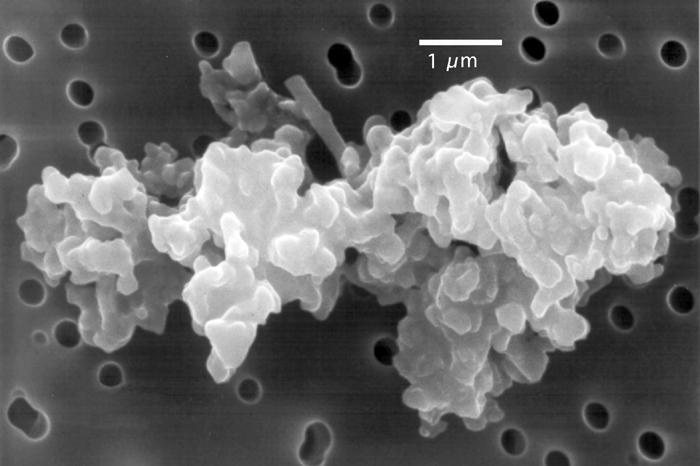
\includegraphics[width=8cm]{figures/grain.jpg}
 	\caption{A scanning electron microscopy (\textit{SEM}) image of a porous chondrite dust grain recovered from high atmosphere.  The authors of this figure are Donald E. Brownlee, University of Washington, Seattle, and Elmar Jessberger, Institut für Planetologie, Münster, Germany.
This file is licensed under CC-BY 2.5 License.}
 	\label{fig:dust_grain}
\end{figure}

\subsubsection{Dust density} \label{sec:density}

Bulk density of the common minerals containing the usual meteorite component elements, such as olivine, quartz or pyroxenes is between $2.6 \, \si{g cm^{-3}}$ and $3.8 \, \si{g cm^{-3}}$ \citep{duda1986minerals}. A lot of interplanetary dust contains ice, which naturally has a bulk density close to $1 \, \si{g cm^{-3}}$.

The density is often assumed between $2.5 \, \si{g cm^{-3}}$ \citep{mann2014dust} and $3 \, \si{g cm^{-3}}$ \citep{mcdonnell1984cosmic}. Dust grains are often, due to photometric and historical reasons described in terms of their linear dimension $d = 2r$, which more often than not means the diameter of the sphere with the volume $V$ equivalent to the dust grain's, hence
\begin{equation}
    \frac{d}{2} = r = \left( {\frac{3V}{4\pi}} \right)^{\frac{1}{3}} \approx 0.62 \sqrt[3]{V}.
\end{equation}
As a general rule, we will use the radius $r$ as the reference to the grain's size, rather than the diameter $d$, throughout this work. Since we meet both mass-based notation and size-based notation, it is useful to keep the conversion in mind, which stands
\begin{equation}
    m = \rho \frac{4\pi}{3} r^3 \Leftrightarrow r = \sqrt[3]{\frac{3 m}{4 \rho \pi}},
    \label{eq:density}
\end{equation}
and assuming $2.5 \, \si{g cm^{-3}}$ gives
\begin{equation}
    \frac{m}{\si{kg}} \approx 10.4 \cdot 10^3 \left(\frac{r}{\si{m}}\right)^3 
\Leftrightarrow 
    \frac{r}{\si{m}} = 4.6 \cdot 10^{-2} \sqrt[3]{\frac{m}{\si{kg}}},
\end{equation}
which is shown in \Figref{fig:mass_size_ruler}.

\begin{figure}[h]
 	\centering
 	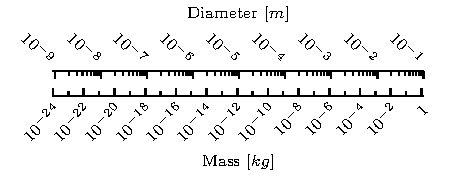
\includegraphics[width=10cm]{figures/mass_size_ruler.pdf}
 	\caption{A conversion between the mass and the radius of a spherical dust grain, assuming the density of $2.5 \, \si{g cm^{-3}}$.}
 	\label{fig:mass_size_ruler}
\end{figure}

\section{Forces} 

\subsection{Gravity} \label{ch:gravity}

Gravity is an attractive pair force between two massive objects of the magnitude of 
\begin{equation}
    F_g = G \frac{M m}{R^2} = \mu \frac{m}{R^2},
\end{equation}
where $G \approx 6.67 \cdot 10^{-11} m^3 kg^{-1} s^{-2}$ is the \textit{gravitational constant}, $R$ is the distance between the objects' centres of mass, and masses $M$ and $m$ belong, by convention, to the more and less massive of the objects, respectively. Alternatively, $\mu = G M$ is known as the \textit{gravitational parameter}, which provides a convenient form for the force, especially if $m \ll M$, as is certainly the case of dust grains, with respect to planets and the Sun. In case of the Sun, $\mu \approx 1.3 \cdot 10^{20} \si{m^3 s^{-2}}$.

Due to the steep dependence of the force on the distance $F_g \propto R^{-2}$, it is often the case that a single central body suffices to describe the net gravity force affecting a smaller body. This concept is known as the \textit{Hill sphere}, which is the sphere of influence around every body in the Solar system, within which the body's gravity is the most relevant contributor to the net gravity, compared against the gravity of the Sun. The approximate planet's Hill radius is equal to the distance to the $L_1$ or the $L_2$ Lagrange point, therefore 
\begin{equation}
    R_H \approx a \sqrt[3]{\frac{m}{3M}},
\end{equation}
where $a$ is the planet's semimajor axis, $m$ is the mass of the planet, and $M$ is the mass of the Sun \cite{sheppard2023new}. For example, Saturn's Hill sphere with the Hill radius of $R_{H;Saturn} \approx 0.4 \, \si{AU}$ is necessary for Saturn to retain is $146$ confirmed moons \citep{sheppard2023new}, as well as its far reaching rings. The rings are an example of a dust system bound to a planet. The Sun is however by far the dominant object in most of the Solar system, especially within $1 \, \si{AU}$, and its gravity is usually the only one that is relevant for the dust grain in question.

Object orbit the Sun on circular orbits, if the magnitude of centrifugal force $F_c$ is equal to the magnitude of gravity $F_g$. This condition gives the \textit{circular speed} $v_c$ needed for the equality: 
\begin{equation}
    \frac{m v_c^2}{R} = \mu \frac{m}{R^2} \Leftrightarrow v_c = \sqrt{\frac{\mu}{R}} \Leftrightarrow R = \frac{\mu}{v_c^2}.
    \label{eq:circular_speed}
\end{equation}
The circular speed $v_c$ at $R = 1 \, \si{AU}$ is $v \approx 29.8 \, \si{km s^{-1}}$. Since gravity ceases with $R \to \infty$ as $F_g \propto R^{-2}$, the work needed in order to escape a gravity well is finite. The minimum energy sufficient for the escape is provided by the \textit{escape speed} $v_e$: 
\begin{equation}
    \frac{m v_e^2}{2} = \frac{\mu m}{R} \Leftrightarrow v_e = \sqrt{\frac{2 \mu}{R}} = \sqrt{2} v_c.
    \label{eq:escape_speed}
\end{equation}

\subsection{Radiation pressure}

The power density of solar radiation at $1 \si{AU}$ is $G_{SC} \approx 1361 \, \si{W m^{-2}}$ \citep{kopp2011new} and corresponds to the radiative power of the Sun $P_{Sun} \approx 3.9 \cdot 10^{26} \, \si{W}$. Dividing $G_{SC}$ by the speed of light $c \approx 3\cdot10^8 \, \si{m s^{-1}}$ gives the radiation pressure of
\begin{equation}
    p_{rp}(1 \si{AU}) = \frac{G_{SC}}{c} \approx 4.5 \cdot 10^{-6} \, \si{Pa},
    \label{eq:radiation_pressure}
\end{equation}
and the resulting radiation pressure force $F_{rp}$ is readily obtained as
\begin{equation}
    F_{rp} = p_{rp} S = \frac{P_{Sun}}{4 c \pi R^2} S = \frac{P_{Sun}}{cR^2} r^2, \label{eq:radiation_pressure_force}
\end{equation}
where $S$ is the Sun-facing cross section of the body of interest, $r$ is the body's radius, and $R$ is the distance of the body from the Sun, whereas in the second equation we also assumed the body to be spherical and the Sun to be a point source: $r \ll R$. A dimensionless parameter $\beta$ is used to describe the relative importance of the two forces:
\begin{equation}
    \beta = \frac{F_{rp}}{F_g}.
\end{equation}
Since $F_{rp}$ directly opposes $F_g$, the net force, denoted \textit{effective gravity}, or $F_{eg}$ is obtained as
\begin{equation}
    F_{eg} = F_g - F_{rp},
\end{equation}
and using $\beta$, we get
\begin{equation}
    F_{eg} = (1-\beta) F_g.
\end{equation}
In the case of the Earth, the radiation pressure force is $F_{rp;Earth} \approx 5.8 \cdot 10^8 \, \si{N}$, which might be compared to the gravity between the Earth and the Sun $F_{g;Earth} \approx 5.2 \cdot 10^{33} \si{N}$, resulting in $\beta_{Earth} \approx 10^{-25}$. 

Interestingly, both $F_g$ and $F_{rp}$ scale with the distance from the Sun as $F \propto {R^{-2}}$, as long as the Sun is assumed a point source of radiation. Therefore, $\beta$ is not a function of the distance from the Sun $R$, and we are permitted to express the effective gravity as 
\begin{equation}
    F_{eg} = (1-\beta) G \frac{M m}{R^2} = (1-\beta) \mu \frac{m}{R^2} = \mu_{e} \frac{m}{R^2},
    \label{eq:effective_gravity}
\end{equation}
where $\mu_{e}$ is the body-specific effective gravitational parameter, taking radiation pressure into account. We see that the laws of orbital motion (for example Eqs. \ref{eq:circular_speed} and \ref{eq:escape_speed}) of radiation pressure affected bodies are going to be the same, albeit with a different gravitational parameter $\mu_e$.

We found that $\beta$ only depends on the properties of the Sun and the body in question, and is therefore body specific. Let us study the dependence of $\beta$ on the size of the body in question $r$. It follows that as long as the aforementioned equations for $F_{g}$ and $F_{rp}$ hold, $\beta$ depends on $r$ as 
\begin{equation} 
    \beta = \frac{\frac{P_{Sun}}{c R^2} r^2}{\mu \frac{m}{R^2}} = \frac{P_{Sun}}{\mu c} \frac{r^2}{\rho V} = \frac{P_{Sun}}{\mu c \rho} \frac{3 r^2}{4 \pi r^3} = \frac{3 P_{Sun}}{4 \pi \mu c \rho} r^{-1},
\end{equation}
therefore $\beta \propto r^{-1}$, which is not surprising, given $F_{g} \propto m \propto r^{3}$ and 
$F_{rp} \propto S \propto r^{2}$. Assuming the density of $\rho \approx 2.5 \si{gcm^{-3}}$ as in Sec. \ref{sec:density}, we find that 
\begin{equation}
    \beta \approx 9.6 \cdot 10^{-7} r^{-1} \, \si{m},
    \label{eq:beta_estimate}
\end{equation}
which gives that for $\beta = 1$, that is the radiation pressure force offsetting the gravity fully, the dust grain has to have the radius of $r \approx 960 \, \si{nm}$. However, Eq. \eqref{eq:radiation_pressure_force} assumes the solar photons are either absorbed, or scattered fully as a spherical wave with their momentum transferred to the body. This holds for absorbing materials if $r \gg \lambda$, where $\lambda$ is the wavelength of the radiation. However, $r \approx 950 \si{nm}$ is comparable to the typical sunlight photons and the assumption does not hold fully. A proper calculation of light scattering is necessary and it depends on the material and shape of the grain. This was done previously by other authors \cite{kimura2003composition} for reasonable materials, see Fig. \ref{fig:kimura_mie}. It was found that the maximum of $\beta$ is reached between $10^{-17} - 10^{-16} \si{kg}$, which corresponds to the radius of $100 - 200 \si{nm}$. In any case, the maximum value of $\beta$ is on the order of unity and lower than unity for much smaller or larger grains.

\begin{figure}[h]
 	\centering
 	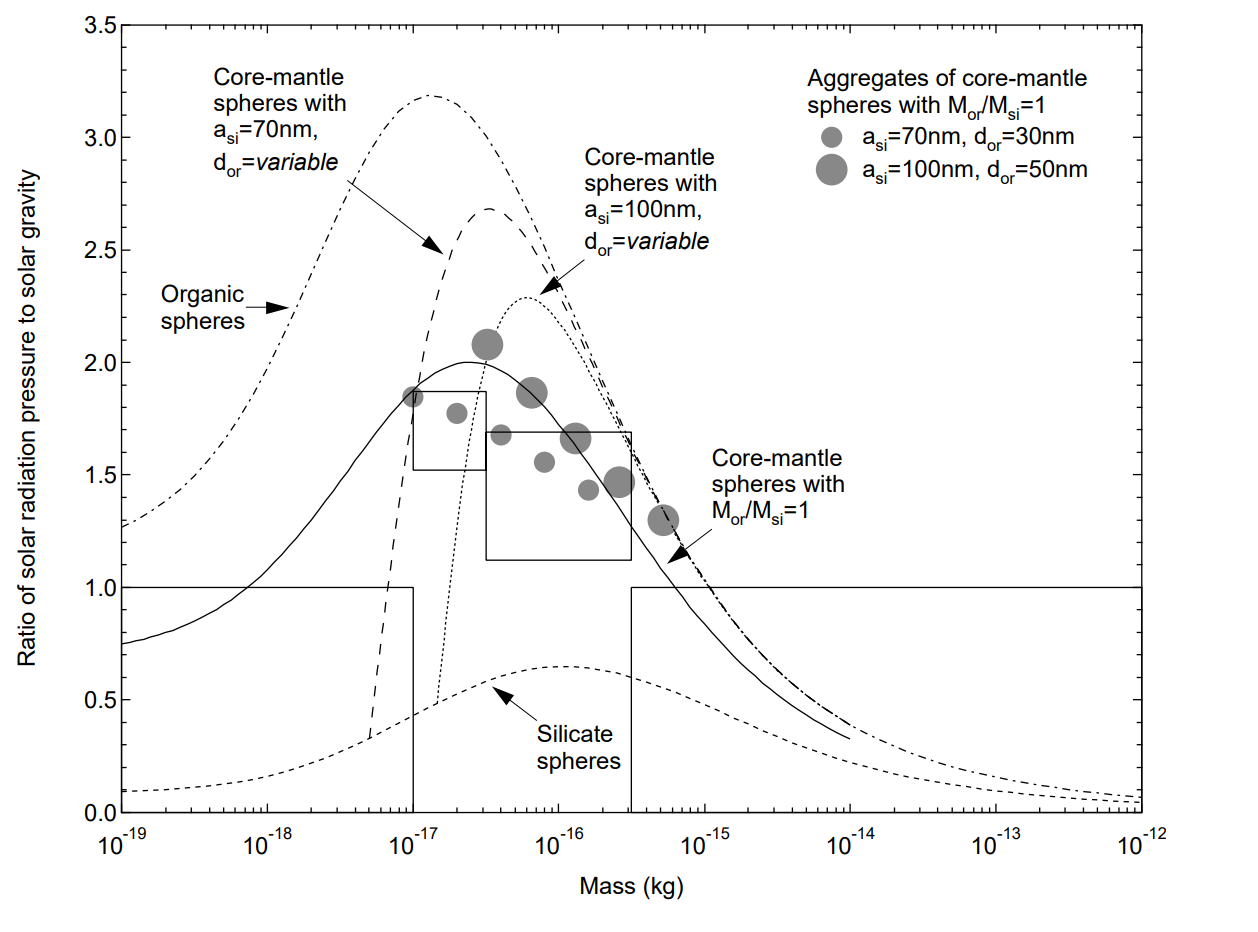
\includegraphics[width=10cm]{figures/kimurra_mie.png}
 	\caption{The light scattering calculation result for the $\beta$ value (\textit{y}-axis) as a function of mass of spherical grains of various composition, adapted from \cite{kimura2003composition}.}
 	\label{fig:kimura_mie}
\end{figure}

\subsection{Lorentz force}

\subsubsection{Grain's potential}

The grains in the solar system are immersed in the ambient plasma and subjected to the solar UV irradiation, both of these causing charging of the grains. Should the ambient conditions remain stable, the grain's electric charge reaches equilibrium. The main charging currents are \textit{electron collection current} and the \textit{photoemission current}. They act to charge the grain to a negative and positive potential respectively. Should the plasma be dense or should the grain be in shadow, the former prevails and the grain's potential becomes negative. Should the plasma be sparse and the UV irradiation dense, the latter prevails and the grain becomes positively charged. We will now examine the two extreme cases. 

An object immersed in plasma charges to so-called \textit{floating potential}. This potential $\phi_{f}$ is typically negative, which is a result of the electron mobility being much higher, compared to the ion mobility. The charging current ceases if the potential of the grain poses a significant barrier to the electrons, therefore the maximum potential is on the order of electron temperature $T_e$, which is approximately $8 \, \si{eV k_B^{-1}}$ near $1 \, \si{AU}$ and $20 \, \si{eV k_B^{-1}}$ near $0.25 \, \si{AU}$ in the typical solar wind \citep{guillemant2013simulation}. 

Electrons are released from an illuminated neutral grain, in case the incident photon's energy $h\nu$ is above the photoelectric work function $W_{p}$ of the grain material. This typically requires UV photons and leaves the grain more positively charged, which adds additional barrier for the next photoelectron to surpass. The established positive potential $\phi_{p}$ is such that no more electrons can escape, therefore it is $\phi_{p} \approx h\nu - W_{p}$. While $W_p$ for common materials is between $2 - 5 \, \si{eV}$, the last strong spectral line of she sunlight is \textit{Ly-$\alpha$} at $h\nu \approx 10.2 \, \si{eV}$, resulting in the maximum potential of $\phi_p$ between $5 - 8 \, \si{V}$. 

The equilibrium potential $\phi$ of the grain depends on the ambient plasma conditions and the properties of the grain, but typically settles on a value between $-20 \, \si{V}$ and $+8 \, \si{V}$. A more comprehensive and careful study is out of scope of this work, but is found in literature \citep{meyer1982flip,horanyi1996charged,krivov1998dynamics,dzhanoev2016charging,vaverka2016lunar}.

\subsubsection{Grain's charge}

An isolated grain's charge $q$ is related to its potential $\phi$ as
\begin{equation}
    q = C \phi, \label{eq:charge}
\end{equation}
where $C$ is the grain's capacitance. The capacitance of a solitary sphere in vacuum with the radius of $r$ is 
\begin{equation}
    C_{sphere} = 4 \pi \epsilon_0 r,
\end{equation}
which translates using Eq. \ref{eq:charge} to
\begin{equation}
    \frac{q}{r \phi} = 4 \pi \epsilon_0 \approx 1.1 \cdot 10^{-10} \, \si{C V^{-1} m^{-1}},
    \label{eq:capacitance}
\end{equation}
where $\epsilon_0 \approx 8.9\cdot10^{-12} \, \si{C V^{-1} m^{-1}}$ is the free space permittivity. This simplistic model predicts the charge of $\pm 10^{-15} \, \si{C}$ for a spherical grain with the radius of $r = 1 \, \si{\mu m}$ at the potential of $\phi = \pm 9 \, \si{V}$. We note that this value is order of magnitude correct for a grain of arbitrary shape with the greatest linear extent of $\approx 2r$. 
The ratio of mass $m$ to charge $q$ is relevant for the dynamics of dust grains. Given the charge as in Eq. \ref{eq:capacitance}, and the mass as in Eq. \ref{eq:density}, we get
\begin{equation}
    \frac{q}{m} = \frac{3 \epsilon_0 \phi}{\rho r^2} \approx 10^{-13} r^{-2} \, \si{m^2},
    \label{eq:charge_estimate}
\end{equation}
where we assumed $\phi \approx 9 \, \si{V}$ and the bulk density $\rho \approx 2.5 \, \si{g cm^{-3}}$ as before. Eq. \ref{eq:charge_estimate} is visualized in Fig. \ref{fig:charge_density_ruler}.

\begin{figure}[h]
 	\centering
 	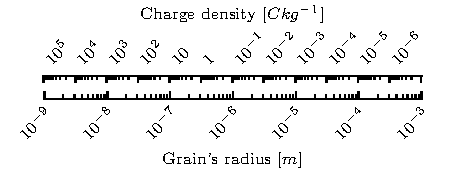
\includegraphics[width=10cm]{figures/charge_density_ruler.pdf}
 	\caption{A conversion between the radius $r$ and the charge density $q/m$ as in Eq. \ref{eq:charge_estimate}.}
 	\label{fig:charge_density_ruler}
\end{figure}

\subsubsection{Dynamics}

A point charge is usually a very suitable model for a charged dust grain. The Lorentz force acting on a point charge $q$ is
\begin{equation}
\vec{F}_{EM} = q \left( \vec{E} + \vec{v} \times \vec{B} \right),
\end{equation}
where $\vec{E}$ and $\vec{B}$ are the ambient electric and magnetic fields respectively, and $\vec{v}$ is the velocity of the point charge. If the charge $q$ is sufficient, $F_{EM}$ might be more important than effective gravity:
\begin{equation}
    F_{eg} < F_{EM} \Rightarrow \frac{q}{m} > \frac{(1-\beta)\mu}{R^2 \left| \vec{E} + \vec{v} \times \vec{B} \right|}. \label{eq:lorentz_gravity}
\end{equation}
As an order of magnitude estimate, let's assume 
\begin{equation}
    F_{EM} \approx q v_{sw} B_{IMF},
    \label{eq:EM_estimate}
\end{equation}
in addition to $\beta = 0$ and $B_{IMF} = 4 \, \si{nT}$, which is a reasonable magnetic field strength near $R = 1 \, \si{AU}$ \citep{mann2007nanoparticles}. This places the condition \ref{eq:lorentz_gravity} to
\begin{equation}
    \frac{q}{m} > 5 \, \si{C kg^{-1}},
\end{equation}
which translates using Eq. \ref{eq:charge_estimate} to $r < 0.14 \, \si{\mu m}$, and is not very sensitive to $R$, provided that $B \propto R^{-2}$, which can often be assumed if $R \gg R_{Sun}$ \citep{parker1958dynamics}.  

This condition describes the state in which Lorentz force is grater in amplitude than gravity. If they are comparable, the curvature in the trajectory of the dust grain due to Lorentz force is similar to the curvature of the trajectory due to the force of gravity, which is on the Solar system scale. We therefore must consider the temporal aspect: given enough time, even $F_{EM} \ll F_g$ might be consequential for the motion of the dust grain, and, vice-versa, $F_{EM} \approx F_g$ does not imply that the grain does not move along a straight line when inspected locally. 

Eq. \ref{eq:lorentz_gravity} has many degrees of freedom. The ratio of $q/m$ is the most important of the grain's properties and the grain's motion is often studied with respect to its $q/m$. \citet{czechowski2010formation} studied the motion of charged grains released in the vicinity of the Sun with the circular speed and charge density of about $10^3 \, \si{C kg^{-1}}$, which corresponds to the radius of $r \approx 10 \, \si{nm}$. The assumed the magnetic field $\vec{B}_{IMF}$ is was described by the Parker spiral \citep{parker1958dynamics} with tilted heliospheric current sheet (\textit{HCS}). They found that if the grains are produced within $0.15 \, \si{AU}$, they remain trapped near the Sun, on non-keplerian orbits with very low aphelia, and therefore are likely destroyed. If the grains are produced outside of $0.2 \, \si{AU}$, they are expelled outward, and their velocity at $1 \, \si{AU}$ depends on their $q/m$, and is on the order of $200 \, \si{km s^{-1}}$ if $q/m \gtrsim 10^3 \, \si{C kg^{-1}}$, and lower for grains with lower $q/m$. 

The motion of dust near the Sun was studied theoretically by other authors, and many effects were described, such as inclination increase \citep{krivov1998dynamics}, ejection \citep{krivov1998dynamics}, and gradual shift of the dust cloud symmetry plane \citep{morfill1979motion}.

\citet{poppe2020effects} studied variability of the flux of dynamically charging $\si{nm}$-sized grains. They made use of electromagnetic field given by a time variable, semi-empirical, corona-solar wind coupled model and found strong variability in the distribution of grains arriving at $1 \, \si{AU}$ within one Carrington rotation. Especially grains with the radius $r<10 \, \si{nm}$ were found to arrive at $1 \, \si{AU}$ with the speed well correlated with the local solar wind speed $v_{sw}$. 

Numerous other publications studied motion of charged grains immersed in the solar system plasma \citep{mann2007nanoparticles,horanyi1996charged,juhasz2013dynamics,stamm2019dust,czechowski2021dynamics,poppe2022effects,rusk1988effect}.

\subsection{Poynting-Robertson drag} \label{ch:pr_drag}

Since an object orbiting the Sun is moving with respect to the source of radiation, the position of the Sun as seen from the object is apparently different, \textit{aberrated}, by an angle of the order of $v/c$, where $v$ is the orbital speed of the object, and $c$ is the speed of light. Therefore, the light doesn't come from pure radial direction, but partially from from the \textit{ram direction}, as observed from the orbiting object. The scattering and absorption of the light then leads to a negative change in the momentum, and therefore in the orbital speed \citep{poynting1903radiation}. The magnitude of Poynting-Robertson effect is \citep{robertson1937dynamical}:
\begin{equation}
    F_{PR} = \frac{v}{c^2} P_{r},
    \label{eq:poynting_robertson}
\end{equation}
where $P_r$ is the power of incoming solar radiation assuming the object's cross section $S$: 
\begin{equation}
    P_{r} = \frac{P_{Sun} S}{4 \pi R^2}.
    \label{eq:radiation_power}
\end{equation}
Assuming the object is on a circular orbit, we make use of Eqs. \ref{eq:poynting_robertson}, \ref{eq:circular_speed}, and \ref{eq:radiation_power} to get
\begin{equation}
    F_{PR} = \sqrt{\frac{\mu}{R}} \frac{P_{r}}{c^2} = \frac{P_{Sun}S}{4 \pi c^2} \sqrt{\frac{\mu}{R^5}}. 
\end{equation}
As an estimate of magnitude of $F_{PR}$, we evaluate the effective pressure $p_{PR}$:
\begin{equation}
    p_{PR} = \frac{F_{PR}}{S} = \frac{P_{Sun}}{4 \pi c^2} \sqrt{\frac{\mu}{R^5}} \approx 4.5 \cdot 10^{-10} \, \si{Pa},
\end{equation}
where we assumed $R \approx 1 \, \si{AU}$, and $c$, $P_{Sun}$, and $\mu$ as before.

As an estimate of relevance of $F_{PR}$, we may study the dynamic evolution of the orbital speed, and, by extension, orbital radius. Although $F_{PR}$ acts against the speed $v$, the speed will actually be rising, as lower energy implies higher orbital speed. Eq. \ref{eq:poynting_robertson} gives for the acceleration $a$ in time
\begin{equation}
    a_{PR}(t) = \frac{dv}{dt}(t) = \frac{P_{r}(t)v(t)}{mc^2} = \frac{P_{Sun} v(t) }{4 \pi R^2(t) c^2} \frac{S}{m},
\end{equation}
where we use the assumption of circularity (Eq. \ref{eq:circular_speed}) once again to get
\begin{equation}
    a_{PR}(t) = \frac{P_{Sun}}{4 \pi \mu^2 c^2} \frac{S}{m} v^5(t),
\end{equation}
which is separable with a single positive real solution for $v(t)$:
\begin{equation}
    v(t) = \left( v(0)^{-4} - \frac{P_{Sun}}{\pi \mu^2 c^2} \frac{S}{m} t \right)^{-\frac{1}{4}},
\end{equation}
which translates to $R$:
\begin{equation}\begin{split}
    R(t) &=  \mu \sqrt{ \left(\frac{R_0}{\mu}\right)^{2} - \frac{P_{Sun}}{\pi \mu^2 c^2} \frac{S}{m} t }
    \\ &= \sqrt{R_0^2 - \frac{P_{Sun}}{\pi c^2} \frac{S}{m} t }.
\end{split}\end{equation}
Assuming a spherical dust grain (Eq. \ref{eq:density}), we get
\begin{equation}
    R(t) = \sqrt{R_0^2 - \frac{P_{Sun}}{\pi c^2} \frac{\pi r^2}{\rho \frac{4\pi}{3} r^3} t } = \sqrt{R_0^2 - \frac{3P_{Sun}}{4 \pi \rho c^2} \frac{t}{r} },
    \label{eq:PR_estimate}
\end{equation}
where the factor of $t/r$, the time-scale of the orbital evolution, is proportional to the grain's linear size. Assuming $P_{Sun},\rho$ as before, $r=1\,\si{\mu m}$ grain will spiral from $R_0=1\,\si{AU}$ down to $R=0.1\,\si{AU}$ in $t=1.7 \cdot 10^3\,\si{yr}$. This time becomes $10^6\,\si{yr}$ if we assume an object with the radius of $r \approx 0.6 \, \si{m}$, therefore $F_{PR}$ is irrelevant for the dynamics of macroscopic object, but relevant for the dynamics of the Solar system's dust cloud. 

We note that circular orbits subjected to $F_{PR}$ remain circular. Briefly, and without mathematical rigor, deceleration in the perihelion does not change the perihelion distance $r_{peri}$, but lowers the aphelion distance $r_{aph}$. This decreases eccentricity $e$. Correspondingly, deceleration in the aphelion lowers $r_{peri}$, doesn't change $r_{aph}$ and therefore increases eccentricity. We note that $F_{PR} \propto v P_r$, and both these factors reach their maximum in the perihelion of an eccentric orbit, and their minimum in the aphelion, therefore eccentricity is gradually reduced and circular orbit's $e=0$ is stable. Rigorous results for non-circular orbits are available in the literature \cite{wyatt1950poynting}. 

\subsection{Solar wind pressure} \label{ch:solar_wind_pressure}

Interplanetary dust grains are in interaction with the solar wind plasma. The solar wind particles are in predominantly radial motion and they therefore project radial pressure $p_{sw}$ on the dust grains, which is in case of a stationary dust grain easily estimated \citep{shue1998magnetopause} as
\begin{equation}
    p_{sw} = n m_p v^2_{sw},  
\end{equation}
where $n$ is the number density of solar wind protons with mass $m_p$, $v_{sw}$ is the solar wind bulk speed, if only solar wind protons are considered and all the protons are assumed to fully pass ther momentum to the grain. Assuming typical $1 \, \si{AU}$ values of $v_{sw} \approx 300 \, \si{km s^{-1}}$, $n \approx 10^7 \, \si{m^{-3}}$, and $m_p \approx 1.67 \cdot 10^{-27} \, \si{kg}$, we get $p_{sw} \approx 1.5 \cdot 10^{-9} \, \si{Pa}$. We note that $p_{sw} \ll p_{rp}$ (see Eq. \ref{eq:radiation_pressure}). Since both pressures scale as $p \propto R^{-2}$ with the heliocentric distance $R$, solar wind pressure in radial direction $p_{sw}$ is typically negligible compared to the radiation pressure $p_{rp}$.

Even though radial effect of solar wind pressure is negligible compared to radiation pressure, its azimuthal component is not, since the orbital speed of a dust grain $v$ is much closer to the solar wind speed $v_{sw}$ than to the speed of light $c$. Considering a dust grain with speed $\vec{v} = \vec{e_r}v_r + \vec{e_\phi}v_\phi$, the force $\vec{F}_{sw} = \vec{e_r}F_{sw,r} + \vec{e_\phi}F_{sw,\phi}$ on the dust grain is \citep{burns1979radiation}
\begin{equation}\begin{split}
    F_{sw,r} &= S p_{sw} \left( 1-\frac{2v_r}{v_{sw}} \right), \\
    F_{sw,\phi} &= S p_{sw} \left( \frac{v_\phi}{v_{sw}} \right).
\end{split}\end{equation}
The force $F_{sw,\phi}$ is often called pseudo-Poynting-Robertson drag, since it acts similarly to $F_{PR}$ discussed in Sec. \ref{ch:pr_drag}. Assuming orbital speed of the Earth $v_\phi \approx 30 \, \si{km s^{-1}}$ and $v_{sw} \approx 300 \, \si{km s^{-1}}$, we find 
\begin{equation}
    p_{sw,\phi} = \frac{F_{sw,\phi}}{S} \approx 1.5 \cdot 10^{-10} \, \si{Pa},
\end{equation}
which is comparable to $p_{PR} \approx 4.5 \cdot 10^{-10} \, \si{Pa}$ at the same heliocentric distance $R = 1 \, \si{AU}$. With more careful treatment, it was estimated that $p_{sw,\phi} \approx 0.22 p_{PR}$ for typical dust grains \citep{whipple1967maintaining}, and more recently it was found that $p_{sw,\phi} > p_{PR}$ for certain grains with radii $r<0.1 \, \si{\mu m}$, and even radial $p_{sw} \approx p_{rp}$ for silicate grains with radii $r<10 \, \si{nm}$, since the cross section with ions is much better than the cross section with sunlight photons for small particles \citep{mukai1982solar}. 

\section{Erosion} \label{ch:erosion}

The mass of a grain evolves abruptly at \textit{collisions} and gradually due to the solar radiaton and the ambient plasma. The solar radiation is responsible for \textit{sublimation}, while the plasma environment, namely solar wind, is responsible for \textit{sputtering}. 

\subsection{Sublimation}

To find under what conditions sublimation is important, we will examine the \textit{black body temperature}, that is the equilibrium temperature of an object in sunlight. We note that the temperature of a dust grain may, depending on the size and composition, differ from the black-body temperature by a factor of $3$, where the deviation is most prominent for grains with the radius $r \ll 1 \, \si{\mu m}$ \citep{myrvang2018temperature}, where scattering effect must be treated carefully. However, for larger grains of common material, the black body temperature is a useful approximation. 

The black body temperature in the vicinity of a star is obtained by comparing the incoming solar radiation $P_{r}$ (Eq. \ref{eq:radiation_power}) and the output power $P_{out}$ of the body:
\begin{equation}
    P_{out} = S_{tot} \sigma T^4,
    \label{eq:stefan_boltzmann}
\end{equation}
where $S_{tot}$ is the emitting surface of the body, $\sigma$ is the Stefan-Boltzmann constant, and $T$ is the temperature of the black body. Eq. \ref{eq:stefan_boltzmann} is the Stefan-Boltzmann law \citep{stefan1879uber,boltzmann1884ableitnung}. Comparing this to Eq. \ref{eq:radiation_power}, we get the condition for the power equality:
\begin{equation}
    \frac{P_{Sun} S}{4 \pi R^2} = S_{tot} \sigma T^4 \Leftrightarrow T =  \frac{1}{2} \sqrt[4]{\frac{P_{Sun}}{\sigma \pi}} \frac{1}{\sqrt{R}} \approx 279 \, \si{K} \left(\frac{R}{\si{AU}}\right)^{-\frac{1}{2}}, 
\end{equation}
where we note $S$ is the cross section of the grain, whereas $S_{tot}$ is the irradiating surface of the grain, and for a sphere $S_{tot} = 4S$. For reference, the melting point of iron is approxiamtely $1800 \, \si{K}$ and the melting point of olivine is between $1500 \, \si{K}$ and $2200 \, \si{K}$, depending on the exact composition \citep{liu1975melting,pinti2015olivine}. The relation as in the equation is shown in Fig. \ref{fig:black_body_temperature}, along with the melting point of water and the highest melting point of olivine.

\begin{figure}[h]
 	\centering
 	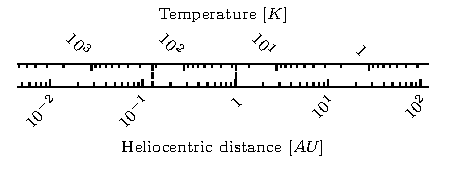
\includegraphics[width=10cm]{figures/distance_temperature_ruler.pdf}
 	\caption{The equilibrium black body temperature as a function of heliocentric distance, assuming spherical body. The temperatures of $273 \, \si{K}$ and $2200 \, \si{K}$ are shown for reference.}
 	\label{fig:black_body_temperature}
\end{figure}

The rate of sublimation of droplets is described by Langmuir's evaporation equation \citep{langmuir1918evaporation}:
\begin{equation}
    \frac{dm}{dt} = -p_{v} S_{tot} \sqrt{\frac{M_e}{2\pi RT}},
\end{equation}
where $p_v$ is the vapor pressure of the droplet fumes at the temperature of the droplets $T$, $S_{tot}$ is the surface of the droplet, $M_e$ is the molar mass of the fumes, and $R$ is the gas constant. This is applicable on dust grains composed of a sublimating material. The parameters $p_v$ and $M_e$ are material-dependent, and the former is also a steeply increasing function of $T$. We note the proportionality to $S_{tot}$, which implies that the sublimation lifetime is proportional to the original radius $r$ of a spherical grain. The differential equation can be solved for initial dust composition and temperature.   

\subsection{Sputtering}

Sputtering is a non-thermal process of erosion of an object due to collisions between the object and energetic particles. Unlike sublimation, sputtering depends on the properties of the plasma environment in addition to the properties of the bombarded object. In the Solar system, the energetic particles are provided by the Sun, in the form of \textit{solar wind} and occasional mass ejections. Sputtering mass loss rate is measured in laboratory as
\begin{equation}
    \frac{dm}{dt} = - \frac{ M_e S \lambda_i Y }{N_A}, 
    \label{eq:sputtering}
\end{equation}
where $M_e$ is the molar mass of the grain's atoms, $S$ is the grain's cross section, $\lambda_i$ is the flux of incident particles, $N_A$ is Avogadro's constant and finally $Y$ is the dimensionless \textit{sputtering yield}, which is modelled as a function of the state of the grain, and energy and mass of the incident particles \citep{vyvsinka2018odpravsovani}. Many assumptions must be done in order to solve the differential equation \ref{eq:sputtering}. 

\subsection{Collisions} \label{ch:collisions}

High-speed collisions between dust grains are inelastic and the mass distribution is changed as the parent grains produce smaller offspring grains. Assume the parent grains have masses $M_1$ and $M_2$, where $M_1 < M_2$. Modelling success was previously achieved \citep{gault1963spray,dohnanyi1969collisional} by assuming so-called \textit{crushing law} to be of the form
\begin{equation}
    g(m) = C(M_1,M_2)m^{-\eta},
    \label{eq:crushing_law}
\end{equation}
where $g(m)$ is a probability density function for the offspring mass $m$, $\eta$ is the power-law exponent, and the factor $C$ is a function of the parent objects' masses. Since the power-law distribution is constrianed by the total amount of collisionally ground material $M_\Sigma$ and is right-bound due to the upper limit of the offspring grain mass $M_{max}$ (that is the largest offspring grain), the normalization is
\begin{equation}
    C(M_1,M_2) = (2-\eta) M_\Sigma M_{max}^{\eta -2}.
\end{equation}
The parameter of $\eta$ was experimentally established \citep{gault1963spray} to be $\eta \approx 1.8$, in case $M_2 \rightarrow \infty$ which implies that most of the offspring mass is retained in the small offspring grains. 
A related modelling concept is that of \textit{catastrophic collisions} \citep{dohnanyi1969collisional,grun1985collisional}. These are collisions which completely shatter both parent grains: $M_\Sigma = M_1 + M_2$. If the smaller of the grains is too small $M_1 \ll M_2$, the bigger grain is not shattered completely. Laboratory experiments have repeatedly shown linearity of the process in mass \citep{gault1963spray,dietzel1973heos,grun1984impact,mcbride1999meteoroid,collette2014micrometeoroid,shen2021cosmic}. In that case, the condition for a catastrophic collision can be written as 
\begin{equation}
    M_2 < \Gamma M_1,
\end{equation}
where the threshold ratio $\Gamma$ is a theoretical concept only, and is a decreasing function of the impact speed and a function of the material properties. It is also difficult to establish experimentally \citep{grun1985collisional}, and different values are found in the literature. For the impact speed of $10 \, \si{km/s}$, the values on the order of $5 \cdot 10^{4}$ were reported \citep{gault1969destruction,fujiwara1977destruction}, but they range from $10^2$ to $5\cdot 10^5$ for broader speed interval \citep{whipple1967maintaining,zook1975source,dohnanyi1978particle}. 
Collisional lifetime of a dust grain is the time it takes for this test dust grain to catastrophically collide with another. This other grain is likely to be smaller than the test grain, since there are many more (by count) small dust grains than large dust grains. Collisional lifetime greatly depends on the mass and speed distribution and to some extent also on the material properties of the dust grains, and is therefore dependent on the heliospheric region. 

\subsection{Lifetimes}

All three erosion processes presented in this section (sublimation, sputtering, and collisions) depend, beyond other assumptions, on the size, the material, and on the location in the Solar system. All three are major factors in shaping the solar system dust cloud's dynamics and are important in different heliocentric regions. 

Due to its speed dependence on the grain's temperature, sublimation prevails in the near vicinity of the Sun. It was evaluated to be dominant within $R < 0.1 \, \si{AU}$, where the sublimation lifetime of $\approx 10^{-1} \, \si{yr}$ is implied for $r \approx 1 \, \si{\mu m}$ silicate dust \cite{baumann2020dust}. Sublimation lifetime is however $\approx 10^{4} \, \si{yr}$ for carbon dust, which has $10^5$-times lower vapor pressure at the temperature of $2300\, \si{K}$. Silicate and metal oxide grains sublimate quickly within $R<0.1\, \si{AU}$, but for carbon dust grains, sputtering and collisions are important even at $0.1 \, \si{AU}$. Let us note that these general results do not cover the instances of high density solar wind, such as during the coronal mass ejections (\textit{CMEs}), which might shorten the lifetime of certain dust grains by a great deal \citep{baumann2020dust}. High mass loss due to sublimation is the most important process behind the formation of so-call near-solar dust depletion zone \citep{russell1929meteoric}. 

Poynting-Robertson drag is not an erosion process on its own, but since it acts to decrease the orbital distance of the grains in orbit around the Sun, it gradually increases the mass loss due to the true erosion processes. As evaluated in Sec. \ref{ch:pr_drag}, the time for $1 \, \si{\mu m}$ particle to spiral down from $R_0 = 1 \, \si{AU}$ to $R = 0.1 \, \si{AU}$ is on the order of $10^3 \, \si{yr}$. It was in fact concluded that while collisions limit the lifetime of grains $r \geq 10^{-4} \, \si{m}$, Poynting-Robertson drag limits the lifetime of the smaller ones \citep{grun1985collisional}. 

It was reported that for the dust of radius $r \approx 1 \, \si{\mu m}$, the collisional lifetime at $1\,\si{AU}$ is on the order of $10^6 \, \si{yr}$, whereas at $0.1\,\si{AU}$ it is on the order of $10^3 \, \si{yr}$ \citep{grun1985collisional}. We can compare this to the sputtering lifetime of silicate grains of the same size, which was calculated to be much shorter at  $\approx 10^4 \, \si{yr}$ at $1\,\si{AU}$, and $\approx 10^2 \, \si{yr}$ at $0.1\,\si{AU}$ even in slow solar wind conditions \citep{klepper2021influence}. It was in fact calculated \citep{klepper2021influence} that the sputtering lifetime is shorter than collisional lifetime between $0.1 \, \si{AU}$ and $1 \, \si{AU}$ for silicate and metal oxide dust grains with $r<20 \, \si{\mu m}$.

To sum up, sublimation limits the lifetime of most grains in the near vicinity of the Sun ($R<0.1 \, \si{AU}$). In most of the inner Solar system, Poynting-Robertson drag limits the life-time of small grains with $r<10^{-3} \, \si{m}$, while collisions limit the life time of larger grains with $r>10^{-3} \, \si{m}$. Sputtering lifetime is comparable, but somewhat longer than Poying-Robertson and collisional lifetimes, except for extreme plasma environments, such as CMEs. A lot more nuanced discussion is found in the literature \citep{klepper2021influence,baumann2020dust,grun1985collisional,whipple1967maintaining,myrvang2018temperature}, which is beyond the scope of this work.  

% Chapter: Dust populations
\chapter{Dust populations}
Different sources of dust, along with different forces acting on dust grains as a result of their location and size, allow us to distinguish \textit{populations} of dust. In this chapter, we are going to discuss several important populations of dust in the Solar system.

\section{Bound dust}

Among the forces discussed in Ch. \ref{ch:forces}, the force with the steepest proportion to the grain's radius $r$ is gravity: $F_g \propto r^3$. Gravity therefore determines the motion of large bodies in the Solar system. The dust particles that are dominantly influenced by the gravity and are in bound orbits, are denoted \textit{bound dust}. The term \textit{zodiacal dust} is sometimes used, since this dust contributes the most to the zodiacal light. The term \textit{F-corona} is used for the zodiacal dust close to the Sun. We may encounter the term \textit{alpha} (abv. $\alpha$) meteoroids, sometimes used interchangeably with bound dust, but appropriateness of the term as a synonym to bound dust was debated \citep{sommer2023alpha}, since the term was originally used to describe highly eccentric bound grains only \citep{zook1975source} and we will not use the term this way.

\subsubsection{Size range}

The size range of interest can be estimated by comparison with the forces dependent $\propto r^2$, namely radiation pressure force $F_{RP}$ and Poynting-Robertson drag $F_{PR}$. If the criterion for $F_{RP} \ll F_g$ is $\beta<0.1$, then using Eq. \ref{eq:beta_estimate} we find $r>10 \, \si{\mu m}$. The Poynting-Robertson time-scale of $r=10 \, \si{\mu m}$ dust (Eq. \ref{eq:PR_estimate}) is approximately $13 \, \si{kyr}$. For completeness, using Eqs. \ref{eq:charge_estimate} and \ref{eq:EM_estimate} we find that for $r=10 \, \si{\mu m}$ dust, the electromagnetic force $F_{EM} < 2\cdot 10^{-4} F_g$. Therefore, the motion of $r>10 \, \si{\mu m}$ dust is dominated by gravity.

Since much larger dust has a low ratio of surface to mass, and since much smaller dust does neither last long in orbit, nor scatters light very effectively, it is the range of $10 \, \si{\mu m} < r < 100 \, \si{\mu m}$ which contributes to the intensity of Zodiacal light the most \citep{leinert1981zodiacal}. 

\subsubsection{Dynamics}

The spatial density of $10 - 100 \, \si{\mu m}$ dust near the ecliptic plane was established based on remote observations to approximately follow 
\begin{equation}
    n(R) \propto R^{-1.3} \label{eq:dust_number_density}
\end{equation}
in the range of $0.3 \, \si{AU} < R < 1 \, \si{AU}$ \citep{leinert1981zodiacal}, and it is believed to be constantly replenished by fragments of colliding, larger, $r \geq 1 \, \si{mm}$ dust with spatial density of $\propto R^{-\nu}$, where $1 < \nu < 1.1$ \citep{leinert1983maintain}.

Bound dust grains are losing mass. This happens gradually, due to erosion, which is faster, if the grains are closer to the Sun. This process is therefore accelerated by shrinking the orbital distance due to Poynting-Robertson drag. The grains also lose mass abruptly, in collisions, as we discussed in Ch. \ref{ch:forces}. It was found that collisions are responsible for the greatest proportion of mass loss from the bound dust population \citep{grun1985collisional}. On the other hand, the population is refilled by dust newly released from comets and in collisions between larger asteroids. Therefore, the bound dust population is believed to be in the state of dynamical balance. 

It was found \citep{dohnanyi1969collisional} that a steady-state mass distribution of asteroids under the influence of erosive and catastrophic collisions with each other (Sec. \ref{ch:collisions}) is established in the power-law form:
\begin{equation}
    f(m) \propto m^{-\delta}, \label{eq:mass_distribution}
\end{equation}
where $\delta = 11/6 \approx 1.83$, provided that the crushing-law (Eq. \ref{eq:crushing_law}) slope $\eta < 2$, that is, there are not too many large objects left after the collision. It is important to note that under the assumption that $\eta < 2$ and that the catastrophic collisions dominate the mass loss, the slope $\delta = 11/6$ is not a function of $\eta$ at all, and is only a very shallow function of $\eta$ if the erosive collisions are relevant. It was also shown that the solution of $\delta = 11/6$ is stable if perturbed by an additional inflow of low or high $m$ into the distribution \citep{dohnanyi1969collisional}. This does not hold fully for the dust grains with $r < \si{\mu m}$, since more loss processes are relevant in this region \citep{grun1985collisional}, most notably, $\beta$-meteoroid production.

\subsubsection{Open questions}

Remote observations provide information about the spatial distribution of dust, while in-situ detections and modelling provide information about its mass distribution. Both are however very insensitive to dust eccentricities and inclinations, therefore to the velocity distribution and the spatial distribution out of the ecliptic plane. While it is generally believed that the dust is concentrated around the ecliptic plane, it is not straightforward to deduce the off-ecliptic density dependence from remote observations and several models were proposed and debated \citep{giese1986three}. Future measurements of Solar Orbiter might shed some light on this, as the spacecraft, which performs in-situ dust measurements, will get gradually inclined between $2025$ and $2029$.

Since the lifetime of dust grains in near vicinity of the Sun is very low due to intense erosion processes (Sec. \ref{ch:erosion}), a dust-free zone (DFZ), enveloped in a dust-depletion zone (DDZ) was hypothesized \citep{russell1929meteoric}. Due to the limitations of the experimental techniques and the difficulties with decomposing the brightness measurements to dust and other light-producing phenomena, the DFZ was not convincingly observed to this date, although the DDZ was from onboard Parker Solar Probe \cite{stenborg2018characterization}. It was recently estimated, based on remote observation from Parker Solar Probe, that the DDZ lies between $5 \, R_{Sun}$ and $19 \, R_{Sun}$, while the DFZ is expected inward of $5 \, R_{Sun}$ \citep{stenborg2022psp}. This implies that the Parker Solar Probe has already travelled well into the DDZ with its perihelia of $\approx 12 \, R_{Sun}$. An investigation of the DDZ was one of the objectives of Paper IV.

\section{Beta meteoroids}

Pioneer 8 and 9 spacecraft discovered a previously unobserved population of dust grains, when it was apparent that most of the grains of the size $r < 10^{-6} \, \si{m}$ were coming from the direction of the Sun \cite{berg1973evidence}. This phenomenon is explained as a population of dust leaving the Sun's gravity well on a hyperbolic trajectory due to the solar radiation pressure successfully competing with solar gravity, and the term \textit{beta meteoroids} ($\beta$ \textit{meteoroids}) was coined as to name the population \cite{zook1975source}. Many other space missions observed the population since, for example \cite{zaslavsky2012interplanetary,malaspina2014interplanetary,zaslavsky2021first}.

\subsubsection{Size range}

As we showed previously (Eq. \ref{eq:effective_gravity}), the laws of motion do not change even if the radiation pressure is significant, it is the effective gravitational parameter $\mu_{e} = (1-\beta) \mu$, which changes with $\beta$. Since the escape speed $v_e$ and the circular speed $v_c$ differ by a factor of $\sqrt{2}$ and both depend on $\mu$ (Eqs. \ref{eq:circular_speed}, \ref{eq:escape_speed}), in terms of effective gravity:
\begin{equation}
    v_c(\beta=0) = v_e(\beta=1/2).
\end{equation}
This implies that if a dust grain on a circular orbit with $\beta=0$ suddenly changes its $\beta$ value to $\beta = 1/2$, it becomes critically unbound, that is on parabolic trajectory. A change to a higher $\beta$ would then naturally lead to a hyperbolic trajectory. Since dust grains change their $\beta$ value suddenly at collisions, and since the post-collision fragment speed is not going to be very different from the pre-collision parent object speed, the value of $\beta=1/2$ is often considered the minimum $\beta$ required for the dust grain to be on an unbound trajectory pointed away from the Sun.

Using our estimate with simplistic assumptions (Eq. \ref{eq:beta_estimate}), $\beta > 0.5$ for $r < 1.9 \, \si{\mu m}$. More refined estimates \citep{kimura2003composition} point to the region of $100 \, \si{nm}$ to $1 \, \si{\mu m}$ and are material dependent. We note that if the parent grains are on eccentric orbits, the requirement of $\beta > 0.5$ is not exact, but this doesn't influence the size estimate greatly. We also note that beta meteoroids are smaller than those, which contribute to the brightness of the Zodiacal light the most. This makes remote observation difficult, and they are therefore, in practice, only detected in-situ.

\subsubsection{Dynamics}

The beta meteoroids are believed to be created in collisions between bound grains, which naturally happens where the bound dust spatial density is high. It was recently reported that the dust detections of Parker Solar Probe are compatible with the beta meteoroid creation region at around $10 - 20 \, R_{Sun}$ \citep{szalay2021collisional}. Since beta meteoroids are unbound, they leave the inner Solar system shortly after their creation, and other forces have limited time to act. For example, even relatively short Poynting-Robertson lifetime of $\approx \, kyr$ is unimportant compared to the timescale of $< 1 \, \si{yr}$, in which a grain created in the vicinity of the Sun passes beyond $1 \, \si{AU}$. On their way out, beta meteoroids follow the conservation of angular momentum and the conservation of energy. The former implies that sufficiently far from the region of their creation, their velocity is nearly purely radial. The latter implies they accelerate if $\beta > 1$, since they feel net solar repulsion, and they decelerate if $\beta < 1$, since they feel net solar attraction. In the special case of $\beta=1$, the grains neither accelerate nor decelerate, and their number density sufficiently far from the Sun depends on the heliocentric distance $R$ as
\begin{equation}
    n(R) \propto R^{-2}. \label{eq:beta_number_density}
\end{equation}
In Paper II of this thesis, we found that the beta meteoroids detected with Solar Orbiter decelerate significantly, which implies effective mean $\beta$ near the liberation threshold, that is $\beta \approx 0.5$. 

\subsubsection{Open questions}

One of the open questions related to beta meteoroids is to what extent is their flux constant in time and rotationally symmetric. Answering this question is complicated, since beta meteoroids are only detected in-situ, and there is always a bond between the time and location of the detecting spacecraft. 

Beta meteoroids were claimed to be produced in collisions between the main, rotationally symmetric bound dust population and the \textit{geminids} meteoric stream \citep{szalay2021collisional}, as a means to explain excess detections with Parker Solar Probe. Further investigation of this phenomenon is desirable.

\section{Interstellar dust}

We know that dust of various sizes is present in the galactic interstellar medium of our galaxy, since it is needed in order to explain the interstellar extinction measurements \citep{desert1990interstellar}. The heliosphere moves with respect to the local interstellar medium, and the relative speed and direction is known, since the velocity distribution of interstellar neutral gas was measured, for example onboard Ulysses spacecraft \citep{witte2004kinetic}. It was also with the Ulysses spacecraft, that a population of dust, seemingly coming from the direction of the interstellar neutral gas was detected \citep{grun1993discovery}. Since then, other spacecraft reported interstellar dust (\textit{ISD}) detections in-situ \citep{zaslavsky2012interplanetary,malaspina2014interplanetary}. 

\subsubsection{Size range and dynamics}

ISD is created by condensation and aggregation, and destroyed by sputtering, sublimation and collisions \citep{mann2010interstellar}. Only the ISD grains with masses higher than $3\cdot 10^{-16} \, \si{kg}$ (that is $r \approx 0.7 \, \si{\mu m} $) are believed to be able to enter the heliosphere \citep{kimura1998electric}. Upon entry, the grains move according to the laws of gravity and under the influence of Lorenz force. The effective gravitational parameter $\mu_e(\beta)$ (see Eq. \ref{eq:effective_gravity}) depends on the amount of radiation pressure compared to gravity. Should $\beta > 1$, the grains are deflected and do not reach close vicinity of the Sun \citep{henriksen2022interstellar}. If $\beta \approx 1$, they do not feel the influence of the Sun and move with nearly constant speed. The motion of the dust grains is also influenced by the Lorentz force, and this effect is also size dependent \cite{morfill1979motion}.

\subsubsection{Open questions}

The exact dynamics of ISD grains in the Solar system is an object of study, especially the possible effect of dust \textit{focusing} and \textit{defocusing} to and from the plane of ecliptics due to the polarity of the interplanetary magnetic field, which switches between N-S and S-N configurations with the period of 22 years, that is two solar cycles \citep{morfill1979motion}. This long period, longer than the duration of many experiments, makes the effect difficult to study. It is however the case that most of the in-situ ISD detections happened around the year 2009, during the solar minimum between the solar cycles 23 and 24, when the interplanetary magnetic field was in the \textit{focusing} configuration \citep{babic2022situ} and the observed ISD flux decreased significantly, although not disappear completely, since then. It was hypothesized that the change in observed flux is physical and that the flux should rise again during the minimum between the solar cycles 25 and 26, which is expected in the late 2020's \citep{mann2010interstellar}. 

Gravitational focusing behind the Sun of the ISD grains with $\beta < 1$ and an increased spatial density in this region is a logical consequence of their trajectories, yet experimental evidence of this is not available \citep{mann2010interstellar}. The low density, the temporal variability and the difficulty of distinguishing this population of dust from beta meteoroids so far prevented the detection.

\section{Nanodust}

Small dust grains are produced in collisions of larger dust. If the created dust grains are so small that $\beta \ll 1$, the radiation pressure does not liberate them from the gravity well of the Sun. Small grains have however high capacitance to mass ratio $C/m$, and by extension, high charge to mass ratio $q/m$. For example $r = 10 \, \si{nm}$ spherical grain at the potential of $\phi = 1 \, \si{V}$ has $q/m \approx 71 \, \si{Ckg^{-1}}$ (Eq. \ref{eq:charge_estimate}). These grains are therefore highly susceptible to be influenced by Lorentz force \citep{czechowski2010formation}. 

As we discussed in Sec. \ref{ch:solar_wind_pressure}, solar wind pressure provides an additional pseudo-Poynting-Robertson drag, which is usually smaller than radiational Poynting-Robertson drag for larger dust, but is likely very relevant for small dust with $r<10\, \si{nm}$ \citep{mukai1982solar}, when even radial solar wind pressure might contest gravity. 

Planetary nanodust was also identified in Cassini/RPWS spectra 
at $\SI{1}{AU}$ \citep{schippers2014nanodust}, and  between $\SI{1}{AU}$ and $\SI{5}{AU}$, and tt was concluded, that the asteroid belt's contribution to the nanodust flux is negligible \citep{schippers2015nanodust}. It was also identified in the jovian system \citep{meyer2009detecting}, and in the saturnian system \citep{kempf2005high}. It was in fact concluded that nanodust is so ubiquitous, that some was detected whenever the RPWS instrument was on \citep{schippers2015nanodust}. Cometary nanodust was detected by Giotto/PIA and Vega/PUMA mass spectrometers net the comet Halley, although very limited information about their composition was yielded, due to low signal \cite{utterback1990attogram}.

\subsubsection{Open questions}

Since nanodust grains are highly susceptible to the influence of Lorentz force, a strong temporal variation is naturally expected, as the inperplanetary magnetic field is not constant \citep{poppe2020effects}. The complications are that nanodust isn't observed remotely, and observation in-situ is complicated \citep{pantellini2012nano,kellogg2016dust,kellogg2017note}. 

Nanodust was reportedly detected on Solar Terrestrial Relations Observatory (\textit{STEREO}) spacecraft \citep{meyer2009dust} and mostly disappear after the solar cycle 24 started after 2010 \citep{zaslavsky2012interplanetary}. It was argued that this might be due to an unfavourable interplanetary magnetic field orientation during the solar cycle 24, and that the nanodust flux will reappear in the STEREO measurements later during the solar cycle 25, at some time before 2028 \citep{poppe2022effects}.

\section{Localized dust}

\subsubsection{Inhomogeneity}

Unlike the omnipresent gradual erosion, the inflow of new dust into the system is very stochastic and non-constant, as for example comets, which are believed to be an important source of the dust cloud, are not uniformly distributed in time and space.

More than a half of all the catalogued comets are so-called \textit{sungrazers}, which are comets which have the perihelion in a close vicinity of the Sun \citep{jones2018science}, at the heliocentric distance of a few solar radii $R_{Sun}$. These are typically small objects ($r<100 \, si{m}$) which don't survive the passage, but are destroyed near the perihelion by the combination of heat and tidal waves. Their material is then partially transferred to the dust cloud. In principle, such highly eccentric comets might arrive from any direction, but a few massive bodies were identified to have been destroyed in the past, which are responsible for most of the identified near-sun comets \citep{jones2018science}. Among these, the most prominent cometary groups is the \textit{Kreutz group} \citep{kreutz1888untersuchungen}, members of which are believed to be descended from a single body, which got fractured in thousands of smaller bodies over several perihelia. The evidence for this is the strong similarity in the orbital elements between the individual Kreutz group comets \citep{jones2018science}, but the exact origin story of the group is not easily established \citep{kalinicheva2017specific,fernandez2021origin}. What is certain is that dust is released from the comets of the group in a spatially highly non-uniform way. 

Meteor is a visual phenomenon accompanying the entry of a sufficiently massive dust grain in the Earth's atmosphere. Over a $100$ distinct meteor showers were identified and confirmed to this day \citep{jenniskens2020removing}, which well document the spatial inhomogeneity of the dust in the Solar system. The number of observed meteors, which belong to shower, is comparable to the number of meteors which do not \citep{jenniskens2016cams}. 

Meteors are caused by comparably large grains of $r \gtrsim \, \si{mm}$ and these are very rare among in situ detections, which are dominated by $r \lesssim \, \si{\mu m}$ grains. These massive and sparse grains however produce smaller grains at collisions, which may be much more frequent where the meteor stream crosses a dense Solar system dust cloud, and this may cause inhomogeneity even in the flux of smaller dust. This effect was proposed as an explanation for the post-perihelion enhancement of flux detected by Parker Solar Probe \citep{szalay2021collisional}. 

\subsubsection{Planetary dust}

The dust directly linked to a planet, is denoted as \textit{planetary dust}. The passage of Pioneers 10 and 11 through the jovian system has discovered flux of dust several orders of magnitude higher than the flux commonly observed elsewhere at the same heliocentric distance \citep{humes1974interplanetary}. The subsequent study by Voyager, which revealed the active volcanism at Io \citep{kruger2004jovian}, and Ulysses, which measured intermittent dust streams origination in the jovian system \citep{grun1993discovery}, confirmed the jovian system as a locally important source of dust. Cassini detected nanodust near Jupiter, which was also confirmed to be originationg at the moon Io \citep{meyer2009detecting}. Similarly in the saturnian system, Enceladus was linked to the tenuous E-ring of Saturn \citep{baum1981saturn}. Cassini data also shown nanodust detections \citep{kempf2005high} and later confirmed the volcanic activity on Enceladus \citep{spahn2006cassini}, which feeds the E-ring of Saturn \citep{kempf2010enceladus}. 



% Chapter: Dust detection
\chapter{Dust detection methods}
The presence of dust in space was hypothesized long ago by \citet{cassini1685} as an explanation for the faint light on the night sky near the plane of ecliptics. Dust was also observed locally, that is \textit{in-situ}, by its interaction with spacecraft since the dawn of the space age, when the concern about the risk it posed to the spacecraft was present \citep{whipple1958meteoritic}. This chapter provides an introduction into dust detection methods in general, and into antenna detected impact ionization in particular, since it is vital for the rest of the present work.

\section{Remote observations}

Since dust grains in space absorb light, they are observed by extinction of light, \citep{desert1990interstellar} allowing for transmission spectroscopy, which is useful on the galactic scale \citep{mann2010interstellar}. In terms of the Solar system, refraction, reflection, and thermal emission by dust is important, since it shows the spatial distribution and size distribution of dust in the zodiacal cloud \citep{allen1946spectrum,hulst1947zodiacal,leinert1981zodiacal,stenborg2018characterization,stenborg2021psp}. Measurements of luminance in principle integrate the luminosity on a line of sight (\textit{LOS}) between the observer and infinity. Most of the luminosity originates near the Sun, where both the dust density and the sunlight are the strongest. However, as the existence of Gegenschein shows \citep{roosen1971gegenschein}, scattering is very angle-dependent. It favors smaller angles and, therefore, the sources closer to the observer, and makes the inversion of LOS luminance into dust density more model dependent and ambiguous \citep{mann2004dust,kneissel1991spatial}. Observations from $\SI{1}{AU}$ are therefore limited, especially a few angular degrees from the Sun. The best results are achieved with measurements closer to the Sun, such as those of the two \textit{Helios} spacecraft \cite{leinert1981zodiacal}, which, as we mentioned in the previous chapter (Eq. \ref{eq:dust_number_density}), found the number density of bound dust between $\SI{0.3}{AU}$ and $\SI{1}{AU}$ scaling as $n(R) \propto R^{-1.3}$. More recently, measurements of the Wide-field Imager for Solar Probe (\textit{WISPR}) confirmed this trend \citep{stenborg2021psp}, and even observed a dust depletion zone within $19 \, R_{Sun} \approx \SI{0.09}{AU}$ \citep{stenborg2022psp}. The measurements are difficult to interpret because the luminance of dust-caused F-corona and dust-independent K-corona are hard to distinguish. 

WISPR observed many phenomena, one of them being the clouds of spacecraft debris liberated by impacts of hypervelocity dust on the insulating carbon foam \citep{malaspina2022clouds}. The carbon thermal insulation is fragile and the debris move slowly enough that the light they scatter is captured in individual shots, allowing for the estimation of their speed, which was found to be on the order of $\si{m s^{-1}}$. Trajectories of the debris were also found to be curved around biased electrical antennas, which is a motion similar to the motion of electrons in \citeauthor{pantellini2012nano} process \citep{pantellini2012nano}, which we hypothesize might be responsible for the double-peak signals reported on SolO in Paper III. 


\section{Impact ionization}

\subsection{Charge generation process}

A very fast impact of a dust grain onto a solid target, such as spacecraft body, releases free charges. This is because of the great energy density at the impact site \citep{shen2021cosmic}. At moderate relative speeds of $v \lesssim \SI{10}{kms^{-1}}$, the ionization is mostly due to surface effects on the grain and on the target \citep{kissel1987ion}. At much higher speeds $v \gtrsim \SI{20}{kms^{-1}}$, the grain is destroyed completely and the ionization is due to the effects in the bulk of the target \citep{hornung1994shock}. For this, shock wave formation in the target at supersonic speed is important \citep{drapatz1974theory}, which concentrates the available energy into the shock front, which makes up a small volume of the target, resulting in high volumetric energy density. 

The first reported observation \citep{friichtenicht1964} of impact ionization followed shortly after the development of the first $MV$ dust accelerator \citep{friichtenicht1962}. The charge leaving the impact site after the impact of carbon and iron dust grains was measured with a pre-amplifier connected to a metallic target. The charge was observed to be quasineutral, and the amount of generated charge $q$ was found consistent with the relation
\begin{equation}
    q \propto m v^3,
\end{equation}
for the velocities  $\SI{2}{kms^{-1}} < v < \SI{15}{kms^{-1}}$, where $m$ is the mass of the grain and $v$ is the impact speed. Later measurements \citep{auer1968,mcbride1999meteoroid,grun1984impact,collette2014micrometeoroid,shen2021cosmic} worked with a more general empirical equation of 
\begin{equation}
    q \propto m^\alpha v^\beta, \label{eq:charge_generation}
\end{equation}
and mostly found $\alpha \approx 1$ and $3 < \beta < 5$, depending on the speed interval and the combination of the grain material and the target material.

\subsection{Laboratory simulation}

The most successful dust accelerators are based on electrostatic acceleration principle, not dissimilar to the ion gun. The latest such device offers the acceleration voltage of up to $\SI{3}{MV}$ \citep{shu20123}, allowing for speeds up to $v\gtrsim \SI{50}{kms^{-1}}$ for $r\lesssim\SI{1}{\mu m}$ grains, measuring both the mass and the charge state of the grain right before it hits the target. It not only allows for study of the impact ionization process \citep{shen2021electrostatic,shen2021laboratory,shen2023variability,nouzak2018laboratory,nouzak2021detection,kovcivsvcak2020effective,collette2014micrometeoroid}, but also for the study of atmospheric ablation \citep{thomas2017experimental,deluca2018ionization,deluca2022differential,tarnecki2023experimentally}. Many aspects of each impact can be measured at the same time, as there is no payload or transmission capacity limitation, such as in the case of spacecraft experiments. Although versatile, accelerator measurements bear disadvantages: the experiment happens in a confined chamber in finite vacuum, the accelerated dust grain is selected randomly from a reservoir, and there is an intrinsic correlation between the speed and the mass of a grain, given the charge and the accelerating voltage are constant \citep{shelton1960electrostatic}. As far as the replication of space environment goes, the plasma conditions (solar wind, UV illumination) can be partially replicated in laboratory \citep{shu20123,horanyi2008surface}, but the noise level in laboratory is never as low as in space. 

\subsection{Dedicated ionization detectors}

The mechanism of impact ionization is used to detect dust impacts on spacecraft. In principle, a surface is located in a chamber, where the entry of charged particles is blocked by a filter, which is however not capable of blocking the entry of dust grains.  The surface is therefore exposed to potential dust impacts, which are the only thinkable source of charge in the chamber. Charge is monitored with a bias collector in the chamber, and whenever it appears, it is due to a dust impact. The first such detector was used on the \textit{OGO 3} mission \citep{alexander1968zodiacal}, and was used many times in forms of variable complexity, some of them resolving the charge and directionality \citep{grun1992galileo,grun1992ulysses,berg1969pioneer} of the incident grains, or even allowing for spectroscopy of the impact plasma \citep{srama2004cassini,sommer2023measuring}. Impact ionization detectors are very sensitive and versatile, and they are used not only in orbit, but also on sounding rockets \citep{gunnarsdottir2019charging,trollvik2019observation} to study smoke particles in the mesosphere. 

\subsection{Non-ionization dust detectors}

\subsubsection{Mechanical methods} 

A penetration method was employed on \textit{Pionner 10} and \textit{11} \citep{humes1980results}. A $\SI{25}{\mu m}$ and a $\SI{50}{\mu m}$ pressurized steel cells were mounted on \textit{Pionner 10} and \textit{11} respectively, $234$ cells on each, counting the impacts of dust grains fast and big enough to penetrate them, which showed by the pressure loss in the cell. Together, these detectors counted $182$ dust impacts, showing clearly higher abundance of dust near Jupiter and Saturn, and concluding that the $\approx \SI{10}{\mu m}$ grains observed between the asteroid belt and Jupiter were not circular and in the ecliptic plane, but rather eccentric or inclined. 

An integration experiment was conducted on the Long Duration Exposure Facility \textit{LDEF} satellite \citep{love1993direct}, which consisted of a study of $\SI{5.6}{m^2}$ aluminium plate exposed to the near Earth environment for nearly six years. In total $761$ craters were found on a microscope scan, allowing for the estimate of the total meteoric mass accretion rate by the Earth to $40 \pm 20 \, \si{kg y^{-1}}$. 

Aerogel, an extremely low-density silica material, was shown to provide gentle enough dissipation of kinetic energy to capture hypervelocity cosimc dust grains intact \citep{tsou1995silica}. The same material was used to recover a dust sample from the \textit{Wild 2} comet, which was achieved by the \textit{Stardust} mission \citep{brownlee2014stardust}. 

\subsubsection{Piezoelectric}

In the early age of in-situ dust science, dust was detected with so-called microphone detectors \citep{alexander1963review}. The principle is very simple, as such device consists of a hard target connected to a piezoelectric element, which acoustically registers each strong enough impact. The detectors were however often sensitive ot other effects, which led to vastly imprecise expectations of dust-induced erosion of spacecraft \citep{whipple1958meteoritic}. 

\subsubsection{PVDF} 

Polyvinylidene fluoride (\textit{PVDF}) is a ferroelectric polymer, hence, a polymer capable of holding a permanent electric dipole. When a thin PVDF foil is perturbed by a dust impact, the dipoles are locally perturbed and the material gets locally depolarized, creating a current spike between the surfaces of the foil. Such detector is sensitive to $r \lesssim \si{\mu m}$ hypervelocity grains and can be made with a relatively large detection area and a very low dead time \citep{tuzzolino1996applications}. The latter was used in \textit{Vega 1} and \textit{Vega 2} missions in the proximity of the comet \textit{Halley} \citep{simpson1988dust}. If calibrated, such detector provides information about the magnitude of the impact, as the amount of released charge depends on the mass and the speed of the incident grain. The Venetia Burney Student Dust Counter \textit{VBSDC} \citep{james2010pvdf}, a device of the \textit{New Horizons} mission based on this principle has reported the dust flux between $\SI{1}{AU}$ and $\SI{50}{AU}$ \citep{bernardoni2022student} and has already been functioning for over $18$ years, since 2006. 

\subsection{Antennas}

Many spacecraft carry electrical antennas, which are, not necessarily by design, sensitive to changes in the potential of the spacecraft body \citep{meyer2017frequency}. The term \textit{antenna detection} is misleading, since it is the whole spacecraft area, which acts as a dust detector. It is then the antennas, which register the free charge created upon impact. The spacecraft body is typically positively charged whenever the spacecraft is in sunlight, due to the current of photoelectrons escaping from the spacecraft body \citep{guillemant2013simulation}. Since the resulting electric field around the spacecraft acts to separate the impact-created charge, attracting negative and repulsing positive charge, the positive potential of the spacecraft is transiently lowered. If the time before the equilibrium is restored is long enough, the impact is registered \citep{mann2019dust}. The first spacecraft to measure these transient signals attributable to dust was was \textit{Voyager 1} in 1980 \citep{scarf1982voyager,aubier1983shot,gurnett1997micron}, and numerous spacecraft, such as \textit{Voyager 2} \citep{gurnett1983micron}, \textit{Vega} \citep{laakso1989impacts}, \textit{DS1} \citep{tsurutani2003dust}, \textit{Cassini} \citep{kurth2006cassini}, \textit{Wind} \citep{malaspina2014interplanetary}, \textit{MAVEN} \citep{andersson2015dust}, \textit{STEREO} \citep{zaslavsky2012interplanetary}, \textit{Cluster} \citep{vaverka2017detection}, and \textit{MMS} \citep{vaverka2018comparison} were shown to be suitable for this analysis, adding a new purpose to their electric antenna measurements. 

Recently, this method was acknowledged during the design phase of the electrical antenna suite of PSP's \textit{FIELDS} \citep{bale2016fields}, and of SolO's Radio and Plasma Waves (\textit{RPW}) \citep{maksimovic2020solar}, making the data a lot more usable for dust identification by design choice \citep{mann2019dust}. Even still, the process is dependent on the impact site, spacecraft's state, the ambient conditions, and the parameters of the grain. The time-domain sampled waveforms carry non-trivial information on these. The interpretation of the waveforms' fine structure in terms of the charge generation and collection process was attempted in Paper III. 

Another method of antenna dust detection was proposed, one based on remote sensing of the grain's own electric field, as it (narrowly) misses an electrical antenna. tbd lesceux, meuris

\citep{meyer2001detecting}


\section{Dust detection in antenna measurements}

A myriad of electrical phenomena happen in the inner Solar system, some of them short in time, such as encounters of electrons holes and related solitary waves \citep{malaspina2013electrostatic,steinvall2019multispacecraft}, which may show in asymmetric or oddly shaped forms \citep{pickett2004solitary}. These were proven to be difficult to distinguish from dust impacts \citep{malaspina2016database,vaverka2018comparison}. Besides, reliably identifying a dust impact with a low signal to noise (\textit{SNR}) ratio is complicated in itself. In this section, several detection approaches are presented.

\subsection{Spectra}

The typical main purpose of an in-situ electric antenna measurement device is detection and analysis of plasma waves. Such measurement's results are typically shown in frequency space, such as in a spectrogram or a scalogram. This is often the main, or even the only data product of the measurement, due to physical limitations of the device or due to a limitation in data transmission capacity, especially for non Earth orbiting spacecraft. This is why the first antenna detection of dust relied on a multi-channel spectrum analyzer \citep{scarf1982voyager}. Since dust signatures are very short-lived, they are visible as short lasting broad-band signals, and therefore they interfere with measurements in many frequency bands. The highest produced frequency $f_{hi}$ is limited by the fastest process, that is the rise of the signal. The rise-time is very variable due to several processes responsible \citep{meyer2017frequency,shen2023variability}, but usually happens in $\tau_{rise} \approx \si{\mu s}$ \citep{meyer2017frequency}, hence implies the frequency of $f_{hi} \approx \si{M Hz}$. The lowest frequency $f_{lo}$ is limited by the slowest related process, that is the equalization of the perturbed potential. The characteristic time $\tau_{decay}$ of the exponentially decaying signal returning to the equilibrium depends on the spacecraft's capacitance $C_{SC}$ and the ambient plasma roughly as 
\begin{equation}    
\tau_{decay} \approx \frac{C_{SC} k_B T_{ph}}{e|I_{e}|} \approx \frac{C_{sc} k_B T_{ph}}{e^2 n_e v_e S_{SC}}, 
\end{equation}
where $k_B T_{ph}$ is the photoelectron temperature, $I_e$ is the ambient electron current on the body of the spacecraft, $n_e$ is the ambient electron number density, $v_e$ is the ambient electron mean speed, $S_{SC}$ is the spacecraft's effective surface, and $e$ is the elementary charge \citep{henri2011observations}. The typical $\SI{1}{AU}$ solar wind conditions yield $\tau_{decay} \approx \SI{100}{\mu s}$, which corresponds to $f_{lo} \gtrsim \SI{10}{kHz}$, but can be longer in sparse plasma, and shorter in dense plasma \citep{vaverka2017detection}. 

Although useful, spectral signatures of dust are always somewhat ambiguous, as the most important feature of short and broad band signal is not too specific and dust might by confused with solitary waves, or even electrical interference. These are however more confidently distinguished in the time domain signal, which is the topic of Paper I. In Paper III, we found the rise and decay time theory, recently developed for the purpose of dust identification in spectra \citep{meyer2017frequency}, capable of explaining many of the characteristic times derived from the time domain waveforms.

\subsection{Time domain identification}

If the spacecraft's electrical measurements are recorded in the time domain with high enough sampling rate, the dust impacts are more recognizable, compared to the frequency domain measurements. The typical features were described previously in laboratory measurements \citep{auer1968,nouzak2018laboratory,shen2021laboratory,shen2023variability}, in spacecraft data \citep{zaslavsky2012interplanetary,kellogg2016dust,vaverka2021ion}, and explained theoretically \citep{zaslavsky2015floating,meyer2017frequency,shen2021electrostatic,babic2022analytical}. The response depends on the antenna configuration \citep{shen2023variability,vaverka2021ion}, especially on whether the antennas are configured in a dipole, when the voltage between two antennas is measured, or in a monopole, when the voltage between one of the antennas and the spacecraft body is measured. Since the spacecraft body usually offers a much bigger target, compared to the antennas, most impact happen on the body. Although both monopoloe and dipole measurements were shown to be sensitive to dust impacts on the spacecraft body, the monopole configuration, when the potential of the body is directly measured against an antenna, is favorable \citep{meyer2014importance,mann2019dust}. 

\subsubsection{Visual identification}

A simplified signature of an impact on the spacecraft body in case of monopole measurement is shown in Fig. \ref{fig:impact_process} and is be briefly described as follows: upon impact, quasi-neutral charge is released in a close proximity to the spacecraft. Due to their lower mass, the electrons in the cloud have much higher speed, than the ions, and the most energetic of them escape the potential well of the spacecraft, leaving the spacecraft somewhat more positive than before. Ions follows, and more of them escape, since they are repulsed by the positive potential of the spacecraft, leaving the spacecraft less positive, than it was before the impact. The net potential has changed, and this change as a function of the equilibrium spacecraft potential was studied in laboratory \citep{collette2016characteristic,kovcivsvcak2020effective}. The new potential of the spacecraft exponentially decays to the original equilibrium. A more elaborate description, directly applied to Solar Orbiter's RPW measurements, is offered in Paper III.

\begin{figure}[h]
 	\centering
 	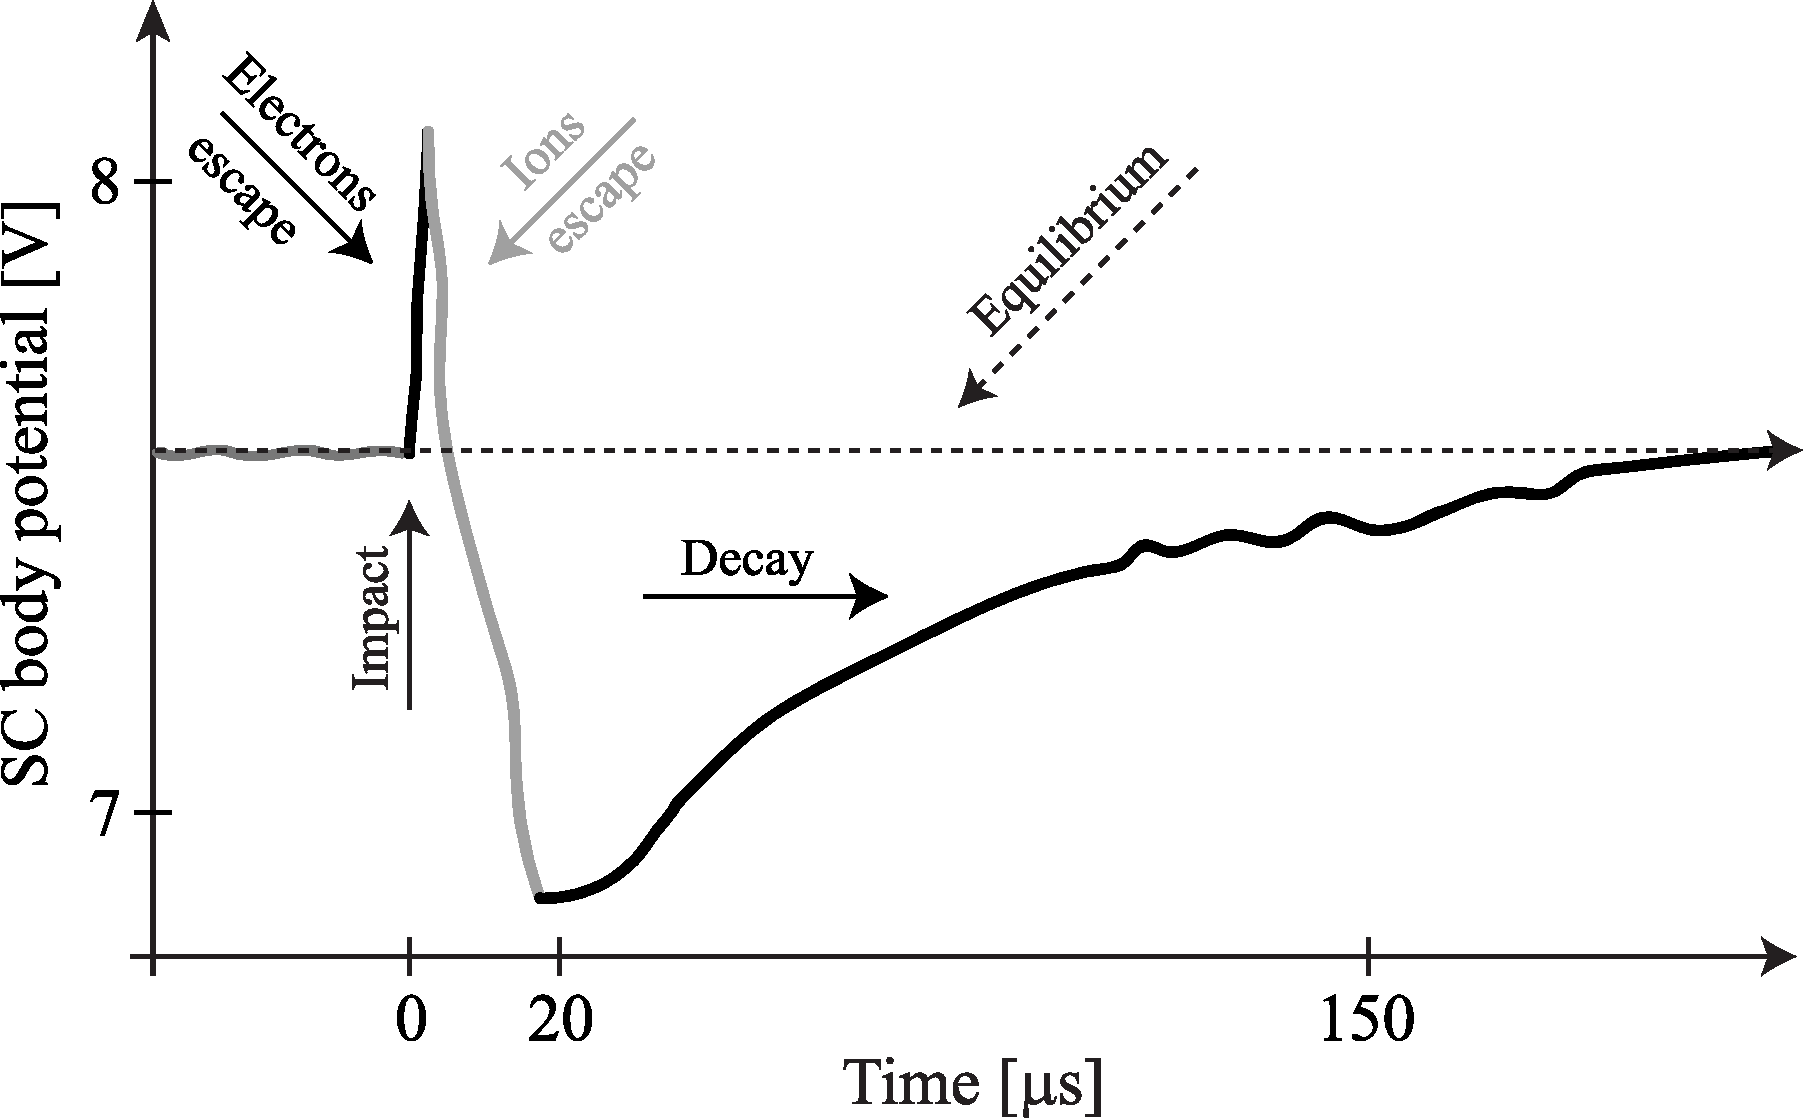
\includegraphics[width=8cm]{figures/impact_wf_gs.pdf}
 	\caption{A simplified dust impact monopole electrical signature after an impact onto a positively charged spacecraft body.}
 	\label{fig:impact_process}
\end{figure}

Therefore, there are several features to look for in the time-domain measurements, such as the quick rise of the signal, and the exponential decay of the maximum. Visual identification is robust to the extent to which experts' opinions on the impact shape agree. Such identification is however very time consuming, and for any reasonably big data set, it is clearly not feasible to use this method alone.

\subsubsection{Hard-coded identification}

The features of dust impact signatures can be translated into algorithmic criteria, which are then efficiently applied to a big data set. While these identification criteria work reasonably well for textbook examples of dust impacts, the actual impacts in space may be quite different from the basic example, as they might contain a lot of noise, saturated data, solitary waves, or a superposition of a dust impact and a wave, and other non-standard signals \citep{vaverka2018comparison,ye2019understanding,malaspina2023dust}. One such algorithm is used for on-board identification of dust impacts on Solar Orbiter \cite{maksimovic2020solar}, and in Paper I, we found this algorithm to be $\SI{94}{\%}$ sensitive and $\SI{79}{\%}$ specific on a sample containing $\SI{50}{\%}$ dust and $\SI{50}{\%}$ non-dust recordings, which was the main motivation for the development of a more reliable automatic identification procedure of that paper. 

\subsubsection{Machine learning}

A supervised machine learning has established itself as a method of time-series classification, particularly in cases, when the exact classification criteria are hard to formulate, but labelled date are abundant \citep{wickstrom2022mixing}. This is a good fit for the problem of dust identification. Methods are available, such as \textit{support vector machine} (SVM), which evaluates a set of pre-defined quantitative features on labelled data, and creates a decision algorithm based on them \citep{vapnik1997support}. \textit{Convolutional neural network} (CNN) is a type of a neural network very useful for the classification of labelled grid-like objects \citep{gu2018recent}. Unlike SVMs, CNNs yield the features vector by convolution operations, and therefore, they don't require a defined feature extracting algorithms. One common disadvantage of CNNs is that they might be difficult to explain, as neural networks generally act like black-boxes, with their internal working hard to interpret. However, great progress was achieved, at least for a limited class of CNNs, in the recent past \citep{samek2021explaining}. If designed to be so, CNN can be explainable to the extent that even features with non-linear effects are interpretable. This not only mitigates the black-box trust issue, but also provides more insight into the problem at hand. In Paper I, both an SVM and an explainable CNN were successfully used to meaningfully improve the performance of the dust identification algorithm, compared to the on-board hard-coded one.

\section{Dust detection flux modelling}

With antenna detection of dust, the whole body of the spacecraft acts as a detection surface for collision between dust grains and the spacecraft. Assuming a 6D phase space probability density function $f(\vec{r},\vec{v})$ for the dust cloud, where $\vec{r}$ is the location and $\vec{v}$ is the velocity of the dust, and normalized to dust number density $n$ as
\begin{equation}
    n(\vec{r}) = \iiint_{\mathbb{R}^3} f(\vec{r},\vec{v}) \,dv_x\,dv_y\,dv_z,
\end{equation}
and a spherical spacecraft with the cross section of $S$, the detection rate $\lambda$ is
\begin{equation}
    \lambda = S \iiint_{\mathbb{R}^3} |\vec{v}-\vec{v}_{sc}| f(\vec{r},\vec{v})  \,dv_x\,dv_y\,dv_z, \label{eq:phase_space_lambda}
\end{equation}
assuming the spacecraft speed $\vec{v}_{sc}$. If the spacecraft moves through a dust cloud with a sharp relative speed between the spacecraft and the dust $v=|\vec{v}_{sc}-\vec{v}|$, the detection rate simplifies to  
\begin{equation}
    \lambda = S n v,
\end{equation}
assuming that the local number density of dust is $n$ and that all the grains are detected, if collided with. In reality, all the collision are never registered, and the higher relative speed $v$ implies a higher charge produced on impact (Eq. \ref{eq:charge_generation}), and in turn higher probability of detection, therefore the rate is sometimes modelled as
\begin{equation}
    \lambda = S n v^{1+\alpha \delta}, \label{eq:rate_semi_general}
\end{equation}
where $\alpha$ is the parameter in charge generation Eq. \ref{eq:charge_generation}, and $\delta$ is the mass distribution slope from Eq. \ref{eq:mass_distribution}. Eq. \ref{eq:rate_semi_general} can be specialized for different dust populations. For example, there is a bond between $\vec{v}_{dust}$ and $r$ for bound dust \citep{szalay2020near}, while $\vec{v}_{dust}$ can be reasonably assumed constant \citep{zaslavsky2021first} for $\beta$ meteoroids, sufficiently far from the Sun. There is also a bond between the number density $n$ and the distance from the Sun for bound dust (Eq. \ref{eq:dust_number_density}) and for $\beta$ meteoroids \ref{eq:beta_number_density}. The number density $n$ and velocity $\vec{v}_{dust}$ of interstellar dust is sometimes assumed constant in space and time. In principle, the cross section $S$ is orientation dependent for non-spherical spacecraft. The total model rate $\Lambda$ in a multi-component model is a superposition of the detection rates $\lambda_i$ for each of the modelled populations as
\begin{equation}
    \Lambda = \sum_{\forall i} \lambda_i,
\end{equation}
where each individual $\lambda_i$ is reasonably approximated. 

Explaining the flux observed on Solar Orbiter with a two component, semi-empirical model, was the goal of Paper II, where we were able to constrain some of the physical parameters of the $\beta$ meteoroids. Building a physics based model for bound dust detections on Parker Solar Probe based on a phase space distribution approach (Eq. \ref{eq:phase_space_lambda}) was the goal of Paper IV and allowed for constraining some of the orbital parameters of the near-solar dust. 

\subsection{Orbital parameters and the data set}

Depending on the orbit of a spacecraft, the observed dust flux is dependent on, and therefore holds the information about different dust populations, while being unable to resolve other populations. We discussed the defining properties of common dust populations in Ch. \ref{ch:populations}. The orbits of selected spacecraft are shown in Fig. \ref{fig:sc_orbits}. In this section, we present different spacecraft, and we explain why their measurements complement each other.  

\begin{figure}[h]
 	\centering
 	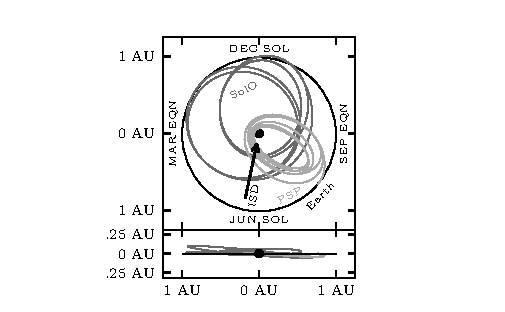
\includegraphics[width=13cm]{figures/solo_orbit.pdf}
 	\caption{The orbit of SolO and PSP in heliocentric (HAE) coordinates between their respective launch date and the summer of 2024, shown in \textit{XY} (top) and \textit{XZ} (bottom) planes. The orbit of the Earth is shown for reference, which is very similar to the orbits of the two STEREO spacecraft. The direction of ISD flow is shown with an arrow.}
 	\label{fig:sc_orbits}
\end{figure}

\subsubsection{Solar Terrestrial Relations Observatory}

The two Solar Terrestrial Relations Observatory (\textit{STEREO}) spacecraft orbit the Sun on a nearly circular orbit close to $\SI{1}{AU}$. Their electrical antenna measurements allow for dust identification \citep{meyer2009dust}. Beyond the intermittent and hard to explain nanodust \citep{meyer2009dust}, the flux was found to be dominated by $\beta$ meteoroids \citep{zaslavsky2012interplanetary}. However, distinguishing $\beta$ meteoroids from bound dust is virtually impossible, since, owing to the circular orbit, the flux of both is expected constant throughout the orbit and the years. This is also an advantage for the detection of interstellar dust (ISD), which is directional, and even though its flux is relatively low, compared to $\beta$ meteoroids, it causes most of the observed variance \citep{zaslavsky2012interplanetary,malaspina2015revisiting,babic2022situ}, with the flux maxima coinciding with the anti-parallel velocity between STEREO and ISD, and minima coinciding with the parallel configuration. Spacecraft located in Earth's L1 point are in just as good position to investigate ISD \citep{malaspina2014interplanetary,malaspina2016database}.

\subsubsection{Solar Orbiter}

SolO orbits the Sun on an elliptical orbit between $\SI{0.3}{AU}$ and $\SI{1}{AU}$ (eccentricity $e \approx 0.52$ in 2024), which means that neither its exposure to bound dust, nor $\beta$ meteoroids is constant. This makes identification of ISD difficult, as it is no longer responsible for an important part of the observed variance. However, the $\beta$ meteoroids are clearly apparent, since the spacecraft's radial speed alternates between negative (pre-perihelia) and positive (post-perihelia), which greatly changes the incidence between the spacecraft and the outgoing $\beta$ meteoroids. Asymmetry in the flux between the inbound and the outbound leg allowed for some of the $\beta$ meteoroid parameters to be constrained by \citet{zaslavsky2021first} and in Paper II. The $\beta$ meteoroids are dominant in the SolO data to the extent that it is not even clear from SolO data alone that bound dust is needed to explain the observed flux.

\subsubsection{Parker Solar Probe}

The orbit of PSP is even more eccentric ($e \approx 0.86$ in 2024), compared to SolO, but even more importantly, PSP gets as close as $\SI{0.052}{AU}$ from the Sun. The relative speed between PSP and the dust components was evaluated by \citet{szalay2020near}, and all suggests that unlike for any other spacecraft, the near-solar dust flux is dominated by bound dust impacts, especially in the post-perihelia. While ISD is difficult to distinguish in SolO data, it is very unlikely to be condifently identified in PSP data, since the variation of the flux on PSP is even much higher, and the alignment is even more unfortunate, with the peak of ISD impacts being nearly aligned with the perihelia (see Fig. \ref{fig:sc_orbits}). The bound dust component, crucial for the flux modelling on PSP, was modelled and constrained in Paper IV. In the paper, we also discuss the different material of the heat shield, and how it likely causes the heat shield to be less sensitive to the impacts. The great variability of the ambient conditions poses additional challenges, as the electric potential, and even conductivity of the spacecraft changes throughout each orbit significantly, which we also investigated and discussed in Paper IV.

\subsection{Compatibility of Solar Orbiter and Parker Solar Probe dust data}

In Paper II, we presented a Bayesian fit of a semi empirical dust flux model to the SolO data from between 6/2020 and 12/2021. As a natural continuation of that effort, in this section, we present a similar fit to the aggregated SolO data from between 6/2020 and 6/2023 and PSP data from between 10/2018 and 7/2023. 

Since the goal is to incorporate measurements from PSP, the model needs to change, as there are physical differences between the spacecraft. Having more data, however, we can afford to fit a somewhat more complicated model, working with six unknowns (hyperparameters). The main changes with respect to Paper II are:
\begin{itemize}
    \item a two component model assuming $\beta$ meteoroids and bound dust is used, as opposed to the two component model assuming $\beta$ meteoroids and a constant background rate used before,
    \item a cuboid shape is assumed for both spacecraft with a different cross section from the front, from the side, and from the back, assuming a motion in the plane of ecliptics, 
    \item while in case of SolO, the cross sections from the front and from the back are assumed equal, in case of PSP, the front side is assumed to have a smaller cross section, due to a different material of the heat shield, as discussed in Paper IV.
\end{itemize}

\begin{table}[t]
\caption{The cuboid-approximation cross section for SolO and PSP. Front side means the heat shield side.}
\centering
\label{tab:cross_section}
\begin{tabular}{c|ccc}
\multicolumn{1}{p{1.2cm}}{  } \vline &  
\multicolumn{1}{p{3cm}}{ \centering $S_{front} \, [m^2]$ } & 
\multicolumn{1}{p{2cm}}{ \centering $S_{side} \, [m^2]$} & 
\multicolumn{1}{p{2cm}}{ \centering $S_{back} \, [m^2]$} \\
\hline
SolO & $10.34$ & $8.24$ & $10.34$   \\
PSP & $6.11 \cdot (1-\alpha_{shield})$ & $4.62$ & $6.11$  \\
\hline
\end{tabular}
\end{table}

We model the detection count per day in case of SolO and per eight hours in case of PSP, and this choice is not very consequential, if it is reasonable to assume the detection rate constant within one detection interval, and an appropriate procedure is used, which is the case. The SolO/RPW data is a product of the CNN procedure presented in Paper I and the PSP/FIELDS data is the data product by \citet{malaspina2023dust}, which is the same data produced as used in Paper IV. The detection count is assumed to come from a Poisson distribution (as in Eq. \ref{eq:poisson_pmf}) and the six-parameter model for the rate, with the free parameters $\lambda_a, \lambda_b, v_{b,r}, \epsilon_v, \epsilon_{b,r}, \alpha_{shield}$ is 
\begin{equation}
    \Lambda = E (\lambda_{bound} + \lambda_{\beta}),
\end{equation}
where $E$ is the exposure time, and the components $\lambda_{bound},\lambda_{\beta}$ are
\begin{equation}\begin{split}
    \lambda_{bound} &= \lambda_a  S(sc,\phi{a}) \left( \frac{|\vec{v}_{a} - \vec{v}_{sc}|}{v_{a,norm}}\right)^{\epsilon_v} \left( \frac{R}{\SI{1}{AU}} \right)^{-1.3} \\
    \lambda_{\beta} &= \lambda_b S(sc,\phi{b}) \left( \frac{|\vec{v}_{b} - \vec{v}_{sc}|}{v_{b,norm}}\right)^{\epsilon_v} \left( \frac{R}{\SI{1}{AU}} \right)^{\epsilon_{b,r}},
\end{split}\end{equation}
where $R$ is the heliocentric distance, and $S(sc,\alpha)$ is the effective cross section, dependent on the spacecraft and the incident angle $\phi$, which in turn depends on the velocity of the dust cloud $\vec{v}_a,\vec{v}_b$ and of the spacecraft $\vec{v}_{sc}$. The bound dust velocity $\vec{v}_a$ is assumed to be purely azimuthal with the speed
\begin{equation}
    |\vec{v}_a| = \left( \frac{R}{\SI{1}{AU}} \right)^\frac{1}{2} \cdot \SI{29.8}{kms^{-1}},
\end{equation}
while the velocity of $\beta$ has two components
\begin{equation}\begin{split}
    \vec{v}_b &= \vec{e}_{rad} v_{b,rad} + \vec{e}_{azim} v_{b,azim} \\
    v_{b,rad} &= \left( \frac{R}{\SI{1}{AU}} \right)^{-2-\epsilon_{b,r}} \, v_{b,r} \\
    v_{b,azim} &= \frac{R}{\SI{1}{AU}} \cdot \SI{9}{kms^{-1}}.
\end{split}\end{equation}
Finally, the speed normalization is done with respect to a stationary (non-orbiting) object at $\SI{1}{AU}$, therefore
\begin{equation}\begin{split}
    v_{a,norm} & = \SI{29.8}{kms^{-1}} \\
    v_{b,norm} & = \left( v_{b,r}^2 + \left(\SI{9}{kms^{-1}}\right)^2 \right)^\frac{1}{2},
\end{split}\end{equation}
where the speed of $\beta$ meteoroids at $\SI{1}{AU}$ of \SI{9}{kms^{-1}} is based on a discussion in Paper II. In this case, the fit was performed by M-H MCMC sampling. The assumed cross sections are based on the projections of the 3D models \citep{psp_model,solo_model} of the two spacecraft and are summarized in Tab. \ref{tab:cross_section}.

\begin{figure}[t]
 	\centering
 	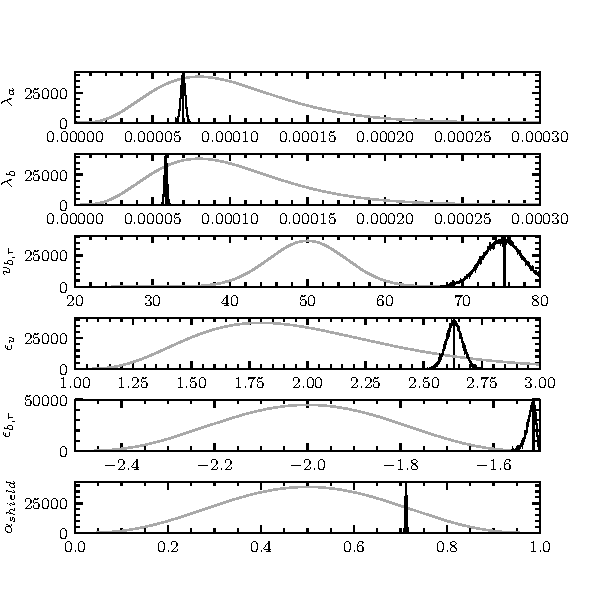
\includegraphics[width=9cm]{figures/both_shield.pdf}
 	\caption{The marginals of the prior (gray) and the posterior (black) of the fit. The posterior is based on a sample of $10^7$ points and the MAP values are indicated with vertical lines. Neither prior nor the posterior are normalized. The summary of both are shown in Tab. \ref{tab:prior_posterior}.}
 	\label{fig:fit_posteriors}
\end{figure}

\begin{table}[t]
\caption{The summary of the prior and the posterior marginals, the same as shown in Fig. \ref{fig:fit_posteriors}.}
\centering
\label{tab:prior_posterior}
\begin{tabular}{c|cc|cc}
\multicolumn{1}{c}{  } \vline & \multicolumn{2}{c}{prior} \vline & \multicolumn{2}{c}{posterior} \\ 
& distribution & support & mean & st. dev. \\
\hline
$\lambda_a$ & $\Gamma(k=5,\theta=2\cdot10^{-5})$ & $\mathbb{R}^+$ &
$6.97 \cdot 10^{-5}$ & $1.4 \cdot 10^{-6}$  \\
$\lambda_b$ & $\Gamma(k=5,\theta=2\cdot10^{-5})$ & $\mathbb{R}^+$ & 
$5.85 \cdot 10^{-5}$ & $8.2 \cdot 10^{-7}$  \\
$v_{b,r}$ & $Norm(\mu=50,\sigma=5)$ & $\mathbb{R}$ & 
$75.3$ & $2.7$  \\
$\epsilon_v$ & $1+\Gamma(k=5,\theta=2\cdot10^{-1})$ & $(1,\infty)$ &
$1.63$ & $3.5 \cdot 10^{-2}$  \\
$\epsilon_{b,r}$ & $-1.5-B(\alpha=4,\beta=4)$ & $(-2.5,-1.5)$ &
$-1.52$ & $9.6 \cdot 10^{-3}$  \\
$\alpha_{shield}$ & $B(\alpha=4,\beta=4)$ & $(0,1)$ & 
$0.71$ & $1.4 \cdot 10^{-3}$  \\
\hline
\end{tabular}
\end{table}

The main shortcomings of the model are the single dust speed assumed, as well as the cuboid approximation. Since the dimension of the model, six, is quite high, we constrained the support of the hyperparameters wherever reasonable. This is, with the transformations used for the prior, indicated in Tab. \ref{tab:prior_posterior}. The priors and posteriors are shown in Fig. \ref{fig:fit_posteriors} and summarized in Tab. \ref{tab:prior_posterior}. They are somewhat different from the results of Paper II, but this is to be expected, since the data is different, as is the model. Therefore, the unknown parameters do not have the exact same meaning as they had in Paper II. The conclusions drawn from the fit in Paper II would not be substantially different, if they were to be drawn from this fit. Interestingly, the PSP heat shield miss rate parameter $\alpha_{shield}$ implies, that the sensitivity of the PSP's front side is by a factor of nearly four lower than the sensitivity of its other sides, and that of SolO. Two things are apparent from Fig. \ref{fig:fit_rate}. First, the model predicts that there is a period present in each post perihelion of PSP, when bound dust dominates the flux. This supports the validity of the analysis done in Paper IV. This is not observed for SolO, for which $\beta$ meteoroids are always dominant. Second, the model is deficient, as it fails to represent the aphelia fluxes of later PSP orbits, where the model flux is higher than observed. We however conclude that both spacecraft do fit in the same framework of a two-component, $\beta$ and bound dust model. 

\begin{figure}[t]
 	\centering
 	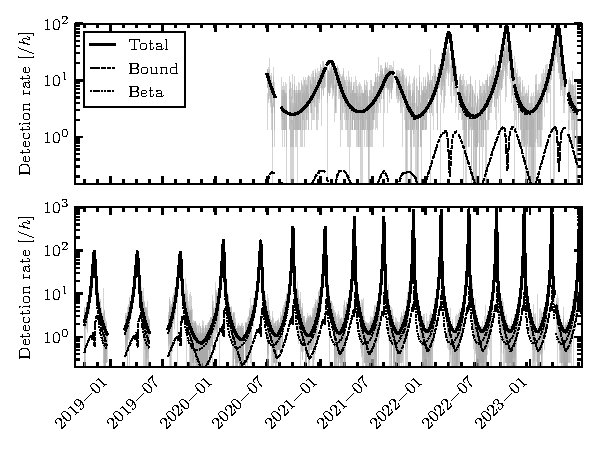
\includegraphics[width=10cm]{figures/both_shield_rate_log.pdf}
 	\caption{The measured impact rate for both spacecraft, where the error bars correspond, for visualization purposes, to $\SI{90}{\%}$ confidence intervals, assuming the rate was the observed $n/E$. The lines correspond to the MAP result of the two-component fit.}
 	\label{fig:fit_rate}
\end{figure}









% Chapter: Impact ionization
\chapter{Impact ionization}
\section{Introduction}

start with energy density, mention shock wave (speed of sound) which concentrates the energy to 2D rather than 3D

\section{Laboratory simulation}

principle, capabilities, limitations (UV missing)

\section{History}

who found what and when. Mostly Friichtenicht, he is the Plato of impact ionization: all the later papers are footnotes to Friichtenicht. 





% Chapter: Antenna detection counts
\chapter{Antenna detection counts}
\section{Dust detection algorithms}

onboard algorithom and introduce CNN and how cnn performs. dont forget to mention spectra

\section{Orbital parameters and the data set}

The trajectory (region, speed, inclination) is important. We will examine SolO and PSP separately, since they are a bit different.

\subsection{Solar Orbiter}

orbits and orbital paramters of SolO to describe what is in the data and what we could have done and what we could not have done. eg escaping population is apparent (beta), but we could never detect ISD due to the alignment. also mention SC potential

\subsection{Parker Solar Probe}

again, what could be extracted from the data and what could not. Meniton the potential and that it is a mess











% In this chapter, a brief derivation of the reduced fluid models used in the included publications is presented. The derivations start from the Braginskii fluid equations whose assumptions and validity for SOL plasmas are discussed. Applying drift reduction, Bohm-normalization and a number of approximations, results in the reduced two-fluid model, equivalent to the two-dimensional fluid models used in Paper III and IV. By applying interchange normalization this model will be further modified to the idealized interchange model, used in Paper I. 

% \section{Braginskii fluid equations}
% The Braginskii fluid model is derived by taking successive velocity moments of the kinetic Boltzmann equation and applying a collisional closure. Each moment depends on the next higher order and therefore require additional assumptions to obtain a closure for the model. The Braginskii equations describe the evolution of the three lowest order fluid moments. The assumptions and the formulation of this closure are presented in \cite{braginskii}. The standard Braginskii fluid equations describing the evolution of the particle density $n_\alpha$, fluid velocity $\textbf{u}_\alpha$ and temperature $T_\alpha$ for particle species $\alpha$ are given by 
% \begin{equation}\label{brag_1}
% 	\frac{\partial n_\alpha}{\partial t} + \nabla \cdot (n_\alpha \textbf{u}_\alpha) = 0,
% \end{equation}
% \begin{equation}\label{brag_2}
% 	m_\alpha n_\alpha \left(\frac{\partial}{\partial t} + \textbf{u}_\alpha \cdot \nabla\right)\textbf{u}_\alpha = - \nabla p_\alpha - \nabla \cdot \Pi_\alpha +Z_\alpha e n_\alpha\left(\textbf{E} + \textbf{u}_\alpha \times \textbf{B}\right) + \textbf{R}_\alpha ,
% \end{equation}
% \begin{equation}\label{brag_3}
% 	\frac{3}{2}n_\alpha \left(\frac{\partial}{\partial t} + \textbf{u}_\alpha \cdot \nabla\right)T_\alpha + p_\alpha \nabla \textbf{u}_\alpha = - \nabla \cdot \textbf{q}_\alpha - \Pi_\alpha : \nabla \textbf{u}_\alpha + Q_\alpha.
% \end{equation}

% Here, $\alpha$ determines the particle species, i.e., electrons and ions, $m$ the particle mass, $p$ the pressure, $Z_\alpha e$ the particle charge, $\textbf{R}$ the friction force, $\Pi$ the viscous stress tensor, $\textbf{q}$ the heat flux, : the tensor inner product and $Q$ the frictional interspecies heating and energy exchange.%, and $S$, $\textbf{S}$ and $W$ represent local density, momentum and energy sources, respectively.
% %In the following, we will focus on the first two moments as all models used in the included papers are isothermal. 

% The Braginskii equations are only applicable if certain assumptions for the modeled system are valid. Applying fluid equations requires that the distribution of particle velocities is close to Maxwellian, i.e., the time scale of relaxation back to a Maxwellian must be shorter than the characteristic time scales of the modeled system. If this condition is fulfilled, the system is referred to as collisional. %This can be expressed as $\omega_c \ll \nu_{ei}$ and $\omega_c \ll \nu_{ii}$ where $\omega_c$ stands for the characteristic frequency of the modeled system and $\nu_{\alpha\beta}$ for the average collision frequency between particle species $\alpha$ and $\beta$. In addition, $l_\parallel \gg \lambda_e$ and $l_\perp \gg \lambda_i$ where $l_\parallel$ and $l_\perp$ represent the smallest length scales of the system parallel and perpendicular to the magnetic field and $\lambda_\alpha$ is the mean free path for a particle species $\alpha$, given by $\lambda_\alpha = v_{\mathrm{th},\alpha}/\nu_{\alpha\beta}$ with the thermal velocity defined as $v_{\mathrm{th},\alpha}= \sqrt{T_\alpha/m_\alpha}$. \textcolor{red}{Ask Fulvio about  i and e}
% In addition to being collisional, a plasma must be strongly magnetized to be adequately described by the Braginskii equations. This implies that the particles complete many gyrations between collisions, setting an upper limit for the collisionality of the plasma. %This condition can be formulated as $\nu_{ie} \ll \Omega_e$ and $\nu_{ii} \ll \Omega_i$ where the gyration frequency is defined as $\Omega_\alpha = eB/m_\alpha$, and $l_\parallel \gg \rho_e$ and $l_\parallel \gg \rho_i$ with the gyration radius given by $\rho_\alpha = v_{\mathrm{th},\alpha}/\Omega_\alpha$. These conditions define the range of time and length scales in which the Braginskii model is valid.

% In summary, the phenomenon we want to model needs to satisfy the following conditions in order to be well described by the Braginskii equations:
% \begin{equation}
% 	L_\perp \gg \rho_\alpha,
% \end{equation}
% \begin{equation}
% 	L_\parallel \gg \lambda,
% \end{equation}
% \begin{equation}
% 	\tau \gg \tau_c \gg \Omega_\alpha^{-1}. 
% \end{equation}
% In these expressions $L_\perp$ stands for the characteristic size of the modeled phenomena perpendicular to the magnetic field, $\rho_\alpha$ is the gyration radius for species $\alpha$, $L_\parallel$ the parallel size of the system, $\lambda$ the collisional mean free path, $\tau$ the characteristic time of the problem, $\tau_c$ the collision time and $\Omega_\alpha$ the gyration frequency of the referred particle species \cite{militellobook}. 

% For the further derivation using drift reduction it will be useful to quantify the magnetization. We thereby define the magnetization parameter $\delta$ as 
% \begin{equation}
% 	\delta = \frac{\rho_\alpha}{L_\perp}.
% \end{equation}
% The magnetization can be equivalently expressed in the temporal domain by 
% \begin{equation}
% 	\delta = \frac{\nu_{ie}}{\Omega_i}
% \end{equation}
% where $\nu_{ie}$ stands for the collisional frequency between ions and electrons.

% For both electrons and ions the magnetization parameter is $\delta \ll 1$ for a fully magnetized plasma. 


% \section{Drift reduction}
% The Braginskii model given by \Eqsref{brag_1} - \eqref{brag_3} is very general, making modeling of SOL plasmas with the presented equations relatively inefficient. A more suitable description of plasma phenomena in the SOL can be derived by simplifying the presented model with an approach called drift ordering. Since turbulence and filaments in the SOL, evolve with velocities much lower than the plasma sound speed $c_s = \sqrt{(T_e+T_i)/m_i}$ we apply the ordering
% \begin{equation}
% 	\textbf{u}_\perp \sim \frac{\rho_\alpha}{L_\perp} c_s \sim \delta c_s.
% \end{equation}
% This ordering assumes that the transverse electric fields are small, resulting in the perpendicular electric field being substantially electrostatic. This is a direct consequence of the $\textbf{E}\times\textbf{B}$ velocity being a factor $\delta$ smaller than sound speed and Faraday's law \cite{militellobook}. We can now determine the perpendicular part of the momentum equation, given by \Eqref{brag_2}, by taking the cross product with $\textbf{B}$ resulting in
% \begin{equation}
% 	\textbf{u}_{\alpha,\perp} = \frac{\textbf{E}\times\textbf{B}}{B^2} - \frac{\nabla p_\alpha \times \textbf{B}}{e_\alpha n_\alpha B^2} - \frac{m_\alpha d \textbf{u}_\alpha/d t \times \textbf{B}}{e_\alpha B^2} - \frac{\nabla \cdot \Pi_\alpha\times\textbf{B}}{e_\alpha n_\alpha B^2} + \frac{\textbf{R}_\alpha \times \textbf{B}}{e_\alpha n_\alpha B^2},
% \end{equation}
% where we used $d/dt = \partial/\partial t + (\textbf{u}_\alpha\cdot \nabla)$ and assumed single charge particle species, i.e., $Z_\alpha e = e_\alpha$. The terms in this expression display the fluid drifts occurring in the system, namely from left to right: the $\textbf{E}\times\textbf{B}$ drift; the diamagnetic drift; the polarization drift; the viscous drift and the collisional drift. From this expression we can determine the dominant drifts and thereby simplify the model.

% As mentioned previously, the electric drift velocity is of $\mathcal{O}(\delta)$ compared to the plasma sound speed:
% \begin{equation}
% 	\textbf{u}_E = \frac{\textbf{E}\times\textbf{B}}{B^2} \sim \delta c_s.
% \end{equation}
% Similarly, the diamagnetic drift is also of $\mathcal{O}(\delta)$ since
% \begin{equation}
% 	\textbf{u}_{\mathrm{dia}} = -\frac{\nabla p_\alpha \times \textbf{B}}{e_\alpha n_\alpha B^2} \sim \frac{n_\alpha T_\alpha B}{L_\perp e_\alpha n_\alpha B^2} \sim \frac{T_\alpha}{L_\perp \Omega_\alpha m_\alpha} \sim \delta c_s.
% \end{equation}
% The polarization drifts for both ions and electrons are smaller in comparison, as can be shown by
% \begin{equation}
% 	\textbf{u}_{\mathrm{pol},i} = \frac{m_i d \textbf{u}_i/d t \times \textbf{B}}{e_i B^2}  \sim \delta^3 c_s,
% \end{equation}
% and
% \begin{equation}
% 	\textbf{u}_{\mathrm{pol},e} \sim \frac{m_e}{m_i} \delta^3 c_s.
% \end{equation}
% For the viscous drift we use Bragniskii's approximation for the perpendicular component of the viscous stress tensor $\Pi_\alpha \sim (p_\alpha/\Omega_\alpha) \nabla v_{\alpha}$ which shows that this term is of $\mathcal{O}(\delta^3)$ since
% \begin{equation}
% 	\textbf{u}_{\mathrm{vis},i} = \frac{\nabla \cdot \Pi_\alpha\times\textbf{B}}{e_\alpha n_\alpha B^2} \sim \frac{nT \delta c_s}{e_i n_i B L_\perp^2 \Omega} \sim \delta^3 c_s,
% \end{equation}
% and
% \begin{equation}
% 	\textbf{u}_{\mathrm{vis},e} \sim \frac{m_e}{m_i}\delta^3  c_s,
% \end{equation}
% respectively. Lastly, we need to find an approximation for the collisional drift. For this we use $\textbf{R}_\perp = e n\,\textbf{J}_\perp/\sigma_\perp$ for the perpendicular momentum transfer from electron-ion friction and $\sigma_\perp = ne^2\nu_{ei}/m_e$. From the ordering follows $\textbf{J}_\perp \sim en\delta c_s$ which leads to the approximation of the frictional drift 
% \begin{equation}\label{diffusion}
% 	\textbf{u}_{\mathrm{fri}} =\frac{\textbf{R}_\alpha \times \textbf{B}}{e_\alpha n_\alpha B^2} \sim \frac{ne\delta c_s}{B \sigma_\perp} \sim \frac{m_e}{m_i}\frac{\nu_{ei}}{\Omega}\delta c_s.
% \end{equation}
% For SOL conditions we can typically assume that $\nu_{ei}/\Omega\sim \delta$ so that the collisional drift is of  $\mathcal{O}(\delta^2)$. 

% This ordering reveals that the dominant perpendicular drifts are the electric and the diamagnetic drifts as all other drifts are at least one order of magnitude smaller. By substituting the remaining drifts into the Braginskii equation we can rewrite the electron density equation in a simpler form,
% \begin{equation}\label{n_e}
% 	\frac{\partial n_e}{\partial t} + \nabla \cdot\left[n_e\left(\textbf{u}_E + \textbf{u}_{\mathrm{dia},e}+ \textbf{u}_{e \parallel}\right)\right] = 0.
% \end{equation}
% Since the plasma is quasi-neutral, i.e.\ $n_e\simeq n_i\simeq n$, this equation is used to describe the evolution of the total plasma density $n$. \Eqref{n_e} is usually manipulated to
% \begin{equation}\label{dens}
% 	\frac{\partial n}{\partial t} + \textbf{u}_E \cdot \nabla n = -\nabla\cdot\left(n\textbf{u}_{\parallel,e}\right) + \left(\frac{1}{e}\nabla p_e - n \nabla \phi\right)\cdot\nabla\times \left(\frac{\textbf{b}}{B}\right).
% \end{equation}
% %As we can see, the diamagnetic drift does not give rise to plasma advection as this term is not a drift of guiding centers but a consequence of counting particle motion through an area in the fluid picture, leading to so called diamagnetic cancellation inside the divergence terms. In non-uniform magnetic fields, this cancellation results in a non-divergence free term $\nabla \times (\textbf{b}/B)$, referred to as the curvature operator, which will be discussed later. 

% Instead of explicitly deriving separate continuity equations for electrons and ions, we can utilize quasi-neutrality and charge conservation to derive an equation for the fluid velocity, which will prove to be very handy. For this we use $\nabla \cdot \textbf{J} = 0$ with $\textbf{J}= e n (\textbf{u}_i - \textbf{u}_e)$. Inserting all drifts that give rise to a net current results in 
% \begin{equation}\label{diff_J}
% 	\nabla \cdot \left(\textbf{J}_{\mathrm{dia}} + \textbf{J}_{\mathrm{pol}} +\textbf{J}_{\mathrm{vis}}+ \textbf{J}_{\parallel}\right) = 0.
% \end{equation}
% In the following we only include the leading order drifts in the ion polarization velocity and neglect the electron polarization drift entirely due to the small electron mass. The sum of the ion polarization and viscous drifts using the lowest order solution
% of the perpendicular momentum equation and the parallel velocity $\textbf{u}_0 = \textbf{u}_{0\perp} + \textbf{u}_{i\parallel}$ is then given by
% \begin{equation}
% 	\textbf{u}_{\mathrm{pol},i} + \textbf{u}_{\mathrm{vis},i} = \textbf{b}\times \frac{1}{enB}\left[m_i n \left(\frac{\partial}{\partial t} + \textbf{u}_{i0} \cdot \nabla\right)\textbf{u}_{i0} + \nabla \cdot \Pi_{i0}\right],
% \end{equation}
% where $\Pi_{i0}$ is the viscous stress tensor calculated with $\textbf{u}_{i0}$ and
% \begin{equation}
% 	\textbf{u}_{0\perp} = \textbf{b}\times \frac{1}{B}\left(\nabla \phi + \frac{1}{en} \nabla p_i \right).
% \end{equation}
% Inserting this into \Eqref{diff_J} leads to the drift-reduced charge conservation equation  \cite{militellobook}
% \begin{multline}\label{charge_conservation}
% 	-\nabla \cdot \left\{\textbf{b}\times\frac{1}{B} \left[m_i n\left(\frac{\partial}{\partial t} + \textbf{u}_{i0}\cdot \nabla\right)\textbf{u}_{i0} + \nabla\cdot \Pi_{i0}\right]\right\} =\\ \nabla\cdot\textbf{J}_\parallel + \nabla \left(p_i + p_e\right) \cdot \nabla\times \left(\frac{\textbf{b}}{B}\right),
% \end{multline}
% which will be further simplified in the following.
% \section{Further approximations and simplifications}
% A number of additional approximations are applied to simplify the model and make it efficiently numerically solvable. 

% First of all, we apply the {electrostatic} approximation, and thereby neglect all time derivatives of $\textbf{B}$ and calculate the electric field $\textbf{E}$ directly from the electric potential. Under this approximation, \Eqref{charge_conservation} can be expressed in the more readable form
% \begin{multline}\label{electrostatic}
% 	m_{i}\nabla\cdot\left[\frac{n}{B} \frac{d_0}{dt}\left(\frac{\nabla_\perp\phi}{B} + \frac{\nabla_\perp p_i}{enB}\right) \right] - \nabla\cdot \left(\textbf{b}\times \nabla\cdot \Pi_0\right) = 
% 	\\ \nabla\cdot\textbf{J}_\parallel + \nabla\left(p_i + p_e\right)\cdot \nabla\times \left(\frac{\textbf{b}}{B}\right),
% \end{multline}
% where we used $d_0/dt = \partial/\partial t + (\textbf{u}_{i0}\cdot \nabla)$. In addition, we neglected spatial non-uniformity of $\textbf{B}$, which will be discussed in further detail later. Studies of electromagnetic effects on plasma blob-filament transport showed that these effects in high temperature or high beta plasmas suppress the resistive drift wave turbulence in filaments \cite{lee2015electromagnetic,hoare2019dynamics} but will not be considered in the following. 

% We can further simplify \Eqref{electrostatic} by applying scale separation for the plasma density, so that $\nabla n \sim \nabla n_0 + \nabla \widetilde{n} \sim 1/L_n + k \widetilde{n}$, where the particle density has been separated into a background $n_0$ and a fluctuation $\widetilde{n}$. $L_n$ stands for the characteristic scale length for the background density and $k$ for the wave number for the particle density fluctuations. Dividing by $n_0$ leads to $\nabla \ln{n} \sim 1/L_n + k \widetilde{n}/n_0$. We now assume that $1/kL_n \ll 1$ and $\widetilde{n}/n_0 \ll 1$. The latter assumption is the so called {thin layer} or {Boussinesq} approximation where we assume that the density perturbations are small compared to the equilibrium. This assumption is hardly justified since relative fluctuations in the SOL can be of order unity as discussed in the previous chapter. This approximation is, however, commonly used since it makes the numerical integration of \Eqref{electrostatic} significantly more efficient. By introducing a generalized vorticity,
% \begin{equation}
% 	\varpi = \nabla\cdot\left(\nabla_\perp \phi + \frac{\nabla_\perp p_i}{en}\right),
% \end{equation}
% we can now simplify the first term in \Eqref{electrostatic} to
% \begin{equation}
% 	m_{i}\nabla\cdot\left[\frac{n}{B} \frac{d_0}{dt}\left(\frac{\nabla_\perp\phi}{B} + \frac{\nabla_\perp p_i}{enB}\right) \right] \approx \frac{m_i n}{B^2}\frac{d_0\varpi}{dt}.
% \end{equation}
% From this expression, $\varpi$ can be relatively easily inverted, especially when assuming that ions are cold, leading us to the next approximation. 

% For the remaining derivation we will assume {small ion temperature}, $T_i \ll T_e$, simplifying the equations significantly. This is a restrictive assumption, as experimental measurements indicate that the ion temperature is higher than the electron temperature in the SOL \cite{kovcan2007ion,kocan2012ion}. Numerical simulations incorporating finite ion temperature have shown that the coherency of filaments is increased \cite{Ahmed_ions}. However, since the simplified model still captures the fundamental dynamics in the SOL, this approximation is commonly used to reduce the model complexity.

% As for the electrons, all models in the included publications and manuscripts assume {isothermal electrons}. This assumption simplifies the model drastically, as it makes \Eqref{brag_3} obsolete. Numerical simulations of isolated filaments with dynamic electron temperature have shown that thermal effects lead to a strong increase in the filament propagation in the poloidal direction and reduce the net radial propagation. These effects arise from the electron temperature dependence of the sheath currents, which will be discussed later in this chapter \cite{walkden2016dynamics}. 

% Next, we will define the geometry of the magnetic field. For the whole simulation domain, we assume {straight magnetic field} lines with {constant} field strength. We need to make one exception to this assumption, as no curvature term would remain in a completely homogeneous field. As there would be no drive for filament motion without this term, it is required to capture some effects of curvature in the model. With the use of vector algebra presented in \cite{militellobook} we can write the curvature term from \Eqsref{dens} and \eqref{electrostatic} as
% \begin{equation}
% 	\nabla\times\left(\frac{\textbf{b}}{B}\right) = 2\frac{\textbf{b}\times{\boldsymbol\kappa}}{B} + \frac{\mu_0\left(\textbf{J}_\parallel - \textbf{J}_\perp\right)}{B^2},
% \end{equation}
% where we introduced the curvature vector $\boldsymbol\kappa = (\textbf{b}\cdot\nabla)\textbf{b}$. Note that one unit of the term $\textbf{b}\times\boldsymbol\kappa/B$ originates from the magnetic gradient and one from the curvature. The second term on the right hand side can be neglected due to charge conservation \cite{militellobook}. The magnetic field in a tokamak can be approximated to lowest order to be purely toroidal and falling radially with $1/R$. In a cylindrical coordinate system $(R,\Phi,Z)$ the toroidal magnetic field is therefore
% \begin{equation}
% 	\textbf{B} = \frac{B_0R_0}{R}\boldsymbol{\widehat{\Phi}}.
% \end{equation}
% In a slab geometry with Z being replaced with the binormal direction $y$ which is perpendicular to $\widehat{\textbf{R}}$ and $\boldsymbol{\widehat{\Phi}}$ this motivates the definition of the curvature operator
% \begin{equation}\label{curvature}
% 	\mathcal{K}(u) = \nabla\times \left(\frac{\textbf{b}}{B}\right)\cdot\nabla u\approx -\frac{2}{B_0R_0}\frac{\partial u}{\partial y}.
% \end{equation}
% %In this expression $R_0$ is defined as the sum of the major and minor radius and $B_0$ the magnetic field strength at that radial position.

% Despite arguing that the frictional drift is negligible in \Eqref{diffusion} one typically retains an approximation of this term due to numerical reasons. We therefore add this term to \Eqref{dens} as 
% \begin{equation}\label{diffusion}
% 	\nabla\cdot \left(n_e \textbf{u}_{\textrm{fri}}\right) \approx -\nabla\cdot \left(D_n\nabla_\perp n_e\right)\approx-D_n\nabla^2_\perp n_e,
% \end{equation}
% where we introduced the density diffusion coefficient $D_n$ which we assumed to be spatially constant. Similarly, one can derive the diffusion term for \Eqref{electrostatic} from its ion viscosity term, since we can use the approximation
% \begin{equation}
% 	\nabla\cdot \Pi_i = -m_in\mu_\omega\nabla_\perp^2\textbf{u}_E,
% \end{equation}
% where $\mu_\omega$ stands for the effective cross-field kinematic viscosity of the ions. Inserting the electric drift and taking the divergence results in the diffusion term for $\nabla_\perp^2\phi$ as
% \begin{equation}
% 	\nabla\cdot\left(\frac{m_i \mu_\omega}{eB^2} \nabla_\perp\nabla_\perp^2\phi\right).
% \end{equation}
% The diffusion coefficients can be approximated from classical or neo-classical diffusion such as presented in \cite{fundamenski2007dissipative}, or are chosen for numerical accuracy and stability. 

% Arguably the starkest simplification of the presented models in this thesis is the restriction to only two dimensions, the plane perpendicular to \textbf{B}. The parallel closure of the model equations is different for closed and open field lines, i.e., whether the simulation domain is located in the SOL or in the edge region. Since the parallel direction plays an important role in the SOL for particle and current dissipation as plasma flows along the magnetic field lines towards the divertor plates, a suitable approximation for the parallel losses is required. This closure is achieved by integrating over the parallel direction where the so-called sheath boundary conditions come into play. In the initial transient period where the plasma vessel is filled and the cold wall surface electrically neutral, electrons will strike the surface at a higher rate than the ions due to their higher speed. This charges the vessel walls negatively which impedes further electron flow towards the surface and results in a thin sheath at material surfaces. Here, the ions shield the electric potential of the surface and the sheath extends a few Debye lengths, $\lambda_D = \sqrt{\epsilon_0T_e/n_ee^2}$, outwards from the surface into the plasma. In this region quasi neutrality is violated since the ion density is higher than the electron density, $n_i > n_e$. The electric current density drawn by the vessel walls is governed by the influx of electrons and ions at the sheath surface. It depends on the potential $\phi$ at the sheath entrance and can be written as
% \begin{equation}\label{parallel_flux}
% 	\textbf{J}_\parallel|_{\mathrm{sheath}} = en_{se}c_s \left[1 - \text{e}^{\Lambda-e{\phi}/{T_e}}\right],
% \end{equation}
% with the plasma density at the sheath edge $n_{se}$, the acoustic speed $c_s$ and the floating potential $\Lambda=\mathrm{ln}\sqrt{m_i/2\pi m_e}$. The first term in the parenthesis is due to the ion flux and the second due to the electron flux \cite{stangeby2000plasma}. %Note that while the ion flux at the sheath edge is given by $n_{se}c_s$, the electron flux is dependent on the potential drop in the sheath \cite{stangeby2000plasma}. 
% We can now take the average of the parallel dimension in a slab geometry with $\textbf{B} = B\, \widehat{\textbf{z}}$,
% \begin{equation}\label{v_parallel}
% \frac{1}{L_\parallel} \int_{-L_\parallel/2}^{L_\parallel/2} \nabla_\parallel \cdot \textbf{J}_\parallel dz,
% \end{equation}
% and use \Eqref{parallel_flux} as the boundary conditions. The first term on the right hand side of \Eqref{dens} can be handled analogously for the parallel electron velocity. 

% Paper III includes a core region in the simulation domain, requiring a different closure for the parallel dynamics. In this model we include resistivity in the parallel component of the electron momentum equation neglecting inertia, i.e.,
% \begin{equation}\label{par}
% 	en\frac{\partial\phi}{\partial z} - T_e\frac{\partial n}{\partial z} + \chi enJ_\parallel=0,
% \end{equation}
% where the resistivity is given by $\chi = m\nu_{ei}/n_e e^2$. %We neglect the parallel ion momentum since the ions remain to lowest order stationary due to their high inertia. 
% Rearranging \Eqref{par} for $J_\parallel$ and taking the parallel derivative results in \cite{bellan2008fundamentals,meyer_thesis}
% \begin{equation}\label{resistivity}
% 	\nabla_\parallel \cdot \textbf{J}_\parallel = \frac{T_e}{e\chi}\frac{\partial^2}{\partial z^2}\left(\mathrm{ln}\,n_e - \frac{e\phi}{T_e}\right).
% \end{equation}
% From this we can take the average of the parallel dimension by integrating over $z$, resulting in the desired 2D model equations. A systematic analysis of the dimensionality of scrape-off layer turbulence is presented in \cite{nicholas_dim,Nicholas2021comparing}.

% \section{Reduced two-fluid model}

% Since the Braginskii fluid model is only valid in a specific range of time and length scales it seems natural to normalize all physical variables to values that are characteristic for the modeled system. We will first discuss the so-called Bohm normalization where we normalize the spatial and temporal units by $\rho_s$ and $\Omega_i$, respectively, i.e.,
% \begin{equation}
% 	\nabla \rightarrow \nabla' = \rho_s\nabla, \,\,\, \frac{\partial}{\partial t} \rightarrow \frac{\partial}{\partial t'} = \frac{1}{\Omega_i}\frac{\partial}{\partial t}.
% \end{equation}
% Here, $\rho_s$ stands for the ion sound Larmor radius defined as $\rho_s = \sqrt{T_e m_i}/eB$.
% We normalize the remaining variables with their characteristic values for SOL conditions $N$ and $T_0$ as
% \begin{equation}
% 	n \rightarrow n' = \frac{n}{N},\,\,\, T_e \rightarrow T' = \frac{T_e}{T_0},\,\,\,\phi \rightarrow \phi' = \frac{e\phi}{T_0}. 
% \end{equation}
% From these expressions we can define the characteristic magnitude for the density source, diffusion coefficients and effective gravity drive as
% \begin{equation}
% 	S\rightarrow S' = SN\Omega_i,\,\,\,D_n\rightarrow D_n' = D_{\textrm{Bohm}}D_n,\,\,\,\mu_\omega\rightarrow D_\Omega' = D_{\textrm{Bohm}}\mu_\omega,\,\,\,g = \frac{2\rho_s}{R},
% \end{equation} 
% where the collisional diffusion is defines as $D_{\textrm{Bohm}}= \rho_s^2\Omega_i$. Applying this normalization to \Eqref{dens} and dropping the dash sign, inserting the curvature operator from \Eqref{curvature} and adding the diffusion term of \Eqref{diffusion} results in the electron density equation
% \begin{equation}
% 	\frac{\mathrm{d}n}{\mathrm{d}t} + g \left(\frac{\partial n}{\partial y} - n\frac{\partial\phi}{\partial y}\right) = D_n \nabla_\perp^2 n + S_n + \Bigg \langle \nabla_\parallel \left(n{u}_{e\parallel} \right)\Bigg \rangle_\parallel,
% \end{equation}
% where the advective derivative is given by $\mathrm{d}/\mathrm{d}t = \partial/\partial t + \textbf{u}_E\cdot \nabla_\perp$ and $\textbf{u}_E = - \nabla_\perp\phi\times\textbf{B}/B^2$ is the $\textbf{E}\times\textbf{B}$ drift. Here, $\langle\cdot\rangle_\parallel$ refers to the average over the parallel dimension. We also added the density source term $S_n$. Performing the same kind of operations on \Eqref{electrostatic} after applying the Boussinesq approximation results in the vorticity equation
% \begin{equation}
% 	\frac{\mathrm{d}\nabla_\perp^2 \phi}{\mathrm{d}t} + \frac{g}{n}\frac{\partial n}{\partial y} = D_{\Omega}\nabla_\perp^4 \phi + \Bigg \langle \frac{1}{n} \nabla_\parallel J_{\parallel} \Bigg \rangle_\parallel,
% \end{equation}
% where we introduced $D_{\Omega}$  as the collisional dissipation term representing viscosity. Averaging over the parallel direction after inserting \Eqref{v_parallel} and \Eqref{resistivity} can be expressed as
% \begin{subequations}
% 	\begin{gather}
% 		\Bigg \langle \nabla_\parallel \left(n{u}_{e\parallel} \right) \Bigg \rangle_\parallel = - \eta(x) n\,\exp(\Lambda-\phi) + \chi(x)( \widehat{\phi} - \widehat{n} ) ,
% 		\\
% 		\Bigg \langle \frac{1}{n} \nabla_\parallel J_{\parallel} \Bigg \rangle_\parallel =  \eta(x) \left[ 1-\exp(\Lambda-\phi) \right] + \chi(x)( \widehat{\phi} - \widehat{n} ),
% 	\end{gather}
% \end{subequations}
% where the spatially fluctuating electron density $\widehat{n}$ and plasma potential $\widehat{\phi}$ are defined as $\widehat{n}=n-\langle{n}\rangle_y$ and $\widehat{\phi}=\phi-\langle{\phi}\rangle_y$ and $\langle{\cdot}\rangle_y$ refers to the flux surface average. Note, that we neglect $1/n$ in the plasma conductivity term for the vorticity equation, since we assume the plasma density to have small relative fluctuation levels in the edge region and $n \sim 1$. We redefined $\chi = \left(\rho_s/L_\parallel\right)^2(m_i/m_e)(\Omega_s/\nu_{ei})$ as the normalized parallel plasma conductivity where we used $\nabla_\parallel^2 \rightarrow -k^2_\parallel\simeq-L_\parallel^{-2}$ and introduced $\eta=\rho_s/L_\parallel$ as the normalized sheath dissipation coefficient. $\nu_{ei}$ stands for the collision frequency between electrons and ions given by
% \begin{equation}
% 	\nu_{ei} = \frac{\textrm{log}\Lambda_c e^4Z^2n_i}{6\sqrt{2}\pi^{3/2} \epsilon_0^2\sqrt{m_e}T_e^{3/2}},
% \end{equation}
% and the Coulomb logarithm is approximately \cite{militellobook}
% \begin{equation}
% 	\textrm{log}\Lambda_c\approx 18 - \textrm{log}\left[\left(\frac{n_e}{10^{19}}\right)^{1/2}\left(\frac{T_e}{10^3e}\right)^{-3/2}\right].
% \end{equation}
% These parameters depend on the radial position, the sheath dissipation term only occurs in the SOL and the plasma conductivity term is finite in the plasma edge region. A schematic illustration of these two regions in the simulation domain is shown in \Figref{Fig:model}.
% \begin{figure}[t]
% 	\centering
% 	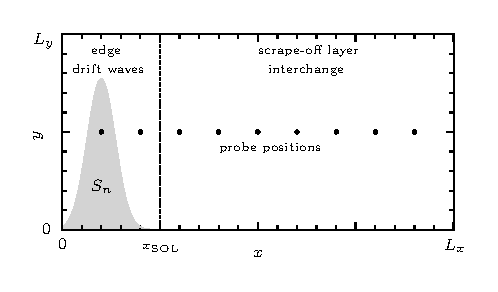
\includegraphics[width=10cm]{figures/model.eps}
% 	\caption{Schematic illustration of the edge and scrape-off layer region in the simulation domain. The position of the plasma
% source term (gray shaded) and the border between edge and SOL (dashed vertical line) are indicated \cite{decristoforo2021numerical}.}
% 	\label{Fig:model}
% \end{figure}

% This model is equivalent to the one used in Paper III. Paper IV utilizes a slightly simpler model placing the whole domain in the SOL by choosing $\eta = \text{constant}$ and $\chi = 0$, and discarding $\Lambda$ in the sheath dissipation term. A list of representative machine parameters relevant for the reduced two-fluid models is presented in Table \ref{tab:machine_parameters}. Since each device performs a range of experiments with slightly different configurations, these parameters might vary. The presented parameters are consistent with those used in the numerical simulations in the included references. The radial position of the SOL is indicated by the sum of the major and minor radius and the parallel connection length is estimated as $L_\parallel = \pi q_{95} R$, with $q_{95}$ as the safety factor  at the 95\% poloidal magnetic flux surface, if not explicitly stated in the references. It should also be noted, that the definition of the connection length varies from source to source as it may refer to the whole poloidal length or only to the lenth between the outboard midplane to the outer divertor plates. 

% \begin{table}[h!]
% 	\begin{center}
% 		\caption{Machine parameters.}
% 		\label{tab:machine_parameters}
% 		\begin{tabular}{c|c c c c c|c} 
% 			 & $n_e[\mathrm{m}^{-3}]$ & $T_e[\mathrm{eV}]$ & $B[\mathrm{T}]$ & $L_\parallel[\mathrm{m}]$ & $R+r[\mathrm{m}]$ & reference\\
% 			\hline
% 			MAST & $8\times 10^{18}$ & 40 & 0.5 & 30 & 1.5 & \cite{easy2016investigation}\\
% 			C-Mod & $1.4\times 10^{19}$ & 23 & 4.5 & 20 & 0.9 & \cite{terry2003observations}\\
% 			TCV & $5\times 10^{18}$ & 25 & 1.45 & 15 & 1.13  & \cite{nespoli2017blob,wensing2019solps}\\
% 			KSTAR & $7\times 10^{17}$ & 35 & 2.0 & 26 & 2.3 & \cite{bak2015investigation} \\
% 			AUG & $8\times 10^{18}$ & 40 & 2.5 & 25 & 2.15 & \cite{militello2011multi} \\
% 			JET & $2\times 10^{19}$ & 45 & 3.45 & 25 & 4.21 & \cite{fundamenski2007dissipative}\\
% 			NSTX & $6\times 10^{18}$ & 13 & 0.25 & 20 & 1.53 & \cite{terry2003observations}
% 		\end{tabular}
% 	\end{center}
% \end{table} 
% The plasma parameters calculated for these device parameters are presented in Table \ref{tab:plasma}.
% \begin{table}[h!]
% 	\begin{center}
% 		\caption{Physical parameters.}
% 		\label{tab:plasma}
% 		\begin{tabular}{c|c c c c} 
% 		 & $\rho_s[\mathrm{m}]$ &$\Omega_i[\mathrm{s}^{-1}]$&$c_s[\mathrm{ms}^{-1}]$\\
% 			\hline
% 			MAST & $1.8\times 10^{-3}$ & $2.4\times 10^{7}$ & $4.4\times 10^{4}$\\
% 			C-Mod& $1.5\times 10^{-4}$ & $2.2\times 10^{8}$ & $3.3\times 10^{4}$\\
% 			TCV & $5.0\times 10^{-4}$ & $6.9\times 10^{7}$ & $3.5\times 10^{4}$\\
% 			KSTAR & $4.3\times 10^{-4}$ & $9.6\times 10^{7}$ & $4.1\times 10^{4}$\\
% 			AUG & $3.7\times 10^{-4}$ & $1.2\times 10^{8}$ & $4.4\times 10^{4}$\\
% 			JET & $2.8\times 10^{-4}$ & $1.7\times 10^{8}$ & $4.6\times 10^{4}$\\
% 			NSTX & $2.1\times 10^{-3}$ & $1.2\times 10^{7}$ & $2.5\times 10^{4}$\\
% 		\end{tabular}
% 	\end{center}
% \end{table}
% Based on these values, we can estimate the input parameters for the reduced two-fluid model shown in Table \ref{tab:input}. Note that the diffusion and viscosity coefficients for the model are not presented as they are chosen arbitrarily high for numerical stability in the included publications.
% \begin{table}[h!]
% 	\begin{center}
% 		\caption{Input parameters.}
% 		\label{tab:input}
% 		\begin{tabular}{c|c c c } 
% 			&  $g$ & $\eta$ & $\chi$ \\
% 			\hline
% 			MAST & $2.4\times 10^{-3}$ &  $6.1\times 10^{-5}$ & $2.7 \times 10^{-4}$\\
% 			C-Mod& $3.4\times 10^{-4}$ &  $7.7\times 10^{-6}$ & $1.0 \times 10^{-5}$\\
% 			TCV & $8.8\times 10^{-4}$ &  $3.3\times 10^{-5}$ & $1.9 \times 10^{-4}$ \\
% 			KSTAR & $3.7\times 10^{-4}$ & $1.6\times 10^{-5}$ & $6.8 \times 10^{-4}$ \\
% 			AUG & $3.4\times 10^{-4}$ & $1.5\times 10^{-5}$ & $7.7 \times 10^{-5}$ \\
% 			JET & $1.3\times 10^{-4}$ & $1.1\times 10^{-5}$ & $3.1 \times 10^{-5}$ \\
% 			NSTX & $2.7\times 10^{-3}$ & $1.0\times 10^{-4}$ & $1.1 \times 10^{-4}$ \\
% 		\end{tabular}
% 	\end{center}
% \end{table}

% \section{Idealized interchange model}
% A minimal model for SOL plasma dynamics in the cross-field plane can be obtained by ignoring parallel dynamics entirely and applying the so called interchange normalization. We start again with \Eqref{dens} and \Eqref{electrostatic}, use the curvature operator given by \Eqref{curvature}, and include the diffusion terms. The perpendicular components then take the form
% \begin{subequations}
% 	\begin{gather}
% 		\left(\frac{\partial}{\partial t} + \frac{1}{B}\widehat{\textbf{z}}\times \nabla\phi\cdot\nabla\right) n - \frac{2n}{B_0 R_0}\frac{\partial \phi}{\partial y} + \frac{2T_e}{eB_0R_0}\frac{\partial n}{\partial y} = D_n\nabla_\perp^2 n,
% 		\\
% 		 \left(\frac{\partial}{\partial t} + \frac{1}{B}\widehat{\textbf{z}}\times \nabla\phi\cdot\nabla\right)\nabla_\perp^2\phi + \frac{2c_s^2}{R_0n}\frac{\partial n}{\partial y} = D_\Omega\nabla_\perp^4 \phi.
% 	\end{gather}
% \end{subequations}
% Under the interchange normalization, length scales are normalized by the characteristic length $l$ of the system, time scales by the ideal interchange rate $\gamma = \sqrt{g/l}$ with $g=2c_s^2/R_0$ and the plasma density and electrostatic potential accordingly, i.e.,
% \begin{equation}
% 	\nabla \rightarrow \nabla' = l\nabla, \,\,\, \frac{\partial}{\partial t} \rightarrow \frac{\partial}{\partial t'} = \frac{1}{\gamma}\frac{\partial}{\partial t}, \,\,\,n \rightarrow n' = \frac{n}{N},\,\,\,\phi \rightarrow \phi' = \frac{\phi}{\gamma B_0l^2}.
% \end{equation}
% Inserting these expressions into the equations for plasma density and vorticity results in 
% \begin{subequations}
% 	\begin{gather}
% 		\left(\frac{\partial}{\partial t'} + \widehat{\textbf{z}}\times \nabla'\phi'\cdot\nabla'\right) n' - 2n'\frac{l}{R_0}\frac{\partial \phi'}{\partial y'} + \frac{\gamma}{\Omega_i}\frac{\partial n'}{\partial y'} = \frac{D_n}{\gamma l^2}{\nabla'}_\perp^2 n',
% 		\\
% 		\left(\frac{\partial}{\partial t'} + \widehat{\textbf{z}}\times \nabla'\phi'\cdot\nabla'\right){\nabla'}_\perp^2\phi' + \frac{1}{n'}\frac{\partial n'}{\partial y'} = \frac{D_\Omega}{\gamma l^2}{\nabla'}_\perp^4 \phi'.
% 	\end{gather}
% \end{subequations}
% We neglect the term resulting from the compression of the electric drift since its prefactor is $l/R_0 \ll 1$. The term resulting from the compression of the diamagnetic drift will also be neglected in the continuity equation as previous work has shown that it has a negligible contribution to the cross-field dynamics and since $\gamma/\Omega_i \ll 1$ \cite{Garcia_thesis}. In addition we introduce the normalized particle diffusion and viscosity coefficients
% \begin{equation}
% 	\kappa = D_n/\gamma l^2 \,\,\,\text{and}\,\,\, \mu = D_\phi/\gamma l^2,
% \end{equation}
% neglect $1/n$ in front of the interchange term as we apply the Boussinesq approximation and drop the dash notation to receive the minimal model for plasma convection 
% \begin{subequations}
% 	\begin{gather}
% 		\left(\frac{\partial}{\partial t} + \widehat{\textbf{z}}\times \nabla\phi\cdot\nabla\right) n = \kappa\nabla_\perp^2 n,
% 		\\
% 		\left(\frac{\partial}{\partial t} + \widehat{\textbf{z}}\times \nabla\phi\cdot\nabla\right)\nabla_\perp^2\phi + \frac{\partial n}{\partial y} = \mu\nabla_\perp^4 \phi.
% 	\end{gather}
% \end{subequations}
% The emphasis of this model lies on reducing the complexity and the number of free parameters as drastically as possible without losing the capability of modeling plasma advection self-consistently. This model has also been used in the past to describe buoyancy-driven convection in a fluid confined between two horizontal plates and heated from below. The model, named the Rayleigh-Bénard convection model after the original experimental work of Henri Bénard \cite{benard1901tourbillons} and the first analytical work on this model of Lord Rayleigh \cite{rayleigh1916lix}, has become a paradigm to investigate nonlinear phenomena due to its rich dynamics \cite{decristoforo2020intermittent, busse1978non,siggia1994high,bodenschatz2000recent,kadanoff2001turbulent,ahlers2009heat}. The normalized particle diffusion and viscosity coefficients in the presented formulation are related to the Rayleigh and Prandtl numbers as $R = 1/\kappa\mu$ and $R=\mu/\kappa$, which are typically used as model parameters for the Rayleigh-Bénard model. We use this model in Paper I.



% Chapter: Poisson rate
\chapter{Fitting Poisson rates}
\section{Poisson random variable}

introducie the pmf, mention PPP

\section{Maximum likelihood estimation}

introduce theoretically and on the example of Poisson pmf

\section{Least squares fitting}

explain under what assumptions this is the MLE, demonstrate how much wrong we will be if we use least squares on poisson distributed data. 

When explaining how scatter is usually fitted leastsq with a linear combination of curves, do the graphics so that curves are being added one after the other so that people understand what is linear combination of the curves, which is very useful for the dissertation presentation - replace that Szalay plot that I used at midterm evaluation

\section{Bayesian estimation}

Introduce Bayes theorem

Introduce Bayesian statistics properly

Exaplain that in higher dimensions, pure minima are rare, therefore MLE is unreliable, and therefore MLE*prior works better

Just mention INLA in the end of this section, phenomenologically












% This chapter is dedicated to describing the Filtered Poisson Process (FPP), a stochastic model used for describing the intermittent fluctuations in single point measurements obtained in the boundary of fusion experiments. The basis of this model was already developed in 1909 \cite{campbell1909study} and was further extended in the 1940s to describe noise in vacuum tubes \cite{rice1944mathematical,rice1945mathematical}. Since then, the model has been extended and used to describe fluctuations in numerous academic fields, including neuroscience, fluid dynamics and nuclear fission 
% \cite{segal1985miniature,fesce1986fluctuation,jang2004martingale,claps2005advances,lefebvre2008generalized,daly2010effect,elter2015performance}. The FPP has first been introduced as a model describing SOL fluctuations in 2012 \cite{garcia2012stochastic} and has since then shown excellent agreement with the statistical properties of fluctuations in various fusion experiments \cite{garcia2013intermittent,garcia2013burst,garcia2015intermittent,kube2016fluctuation,garcia2017sol,kube2018intermittent,garcia2018intermittent,theodorsen2018universality}. 

% \section{Filtered Poisson Process}
% The FPP is a stochastic process, given by a superposition of uncorrelated pulses which are distributed according to a Poisson process. For a given time $t \in [0,T]$ the process $\Phi_k(t)$ can be written as \cite{garcia2012stochastic,garcia2016stochastic}
% \begin{equation}
% 	\Phi_k(t) = \sum_{k=1}^{K(T)} A_k \,\phi\left(\frac{t-t_k}{\tau_\mathrm{d}}\right).
% \end{equation}
% Here, the random variables are defined as follows: $K(T)$ stands for the number of pulses arriving in the time interval $[0,T]$, $A_k$ is the pulse amplitude and $t_k$ the pulse arrival time. It is further assumed that all pulses have the same pulse  shape $\phi$ and duration time $\tau_\mathrm{d}$.

% Alternatively, the process can be expressed as a convolution of the pulse shape and a delta pulse train
% \begin{equation}\label{conv}
% 	\Phi_k(t) = [\phi * f_K] \left(\frac{t}{\tau_\mathrm{d}}\right),
% \end{equation}
% where $f_K$ is the forcing defined as a train of delta pulses
% \begin{equation}
% 	f_K(\theta) = \sum_{k=1}^{K(T)} A_k \,\delta\left(\theta - \frac{t_k}{\tau_\mathrm{d}}\right).
% \end{equation}
% As the process can be expressed as a train of delta pulses filtered through the pulse shape, it is called a \textit{Filtered Poisson Process}. 

% For a given time interval $[0,T]$, the number of pulses $K(T)$ follows a Poisson distribution \begin{equation}
% 	P_K(K|T) = \frac{1}{K!} \left(\frac{T}{\tau_\mathrm{w}}\right)^K \textrm{exp}\left(-\frac{T}{\tau_\mathrm{w}}\right),
% \end{equation}
% with intensity $T/\tau_\mathrm{w}$. The waiting times between two consecutive pulses are independent and exponentially distributed with mean value $\tau_\mathrm{w}$ and the arrival times $t_k$ are independent and uniformly distributed in the interval $[0,T]$. These properties of the process are consistent with experimental measurements, showing exponentially distributed waiting times \cite{garcia2015intermittent,kube2018intermittent,garcia2017sol,garcia2018intermittent}. Time series with quasi-periodic arrival times are observed in SOL simulations utilizing Rayleigh–Bénard like convection models \cite{decristoforo2020intermittent} and are discussed in Paper II in further detail. The amplitudes are chosen to be exponentially distributed, as this is observed in experimental measurements \cite{kube2018intermittent,garcia2017sol,garcia2018intermittent}.

% In the following, we will discuss two pulse shapes that are most relevant for SOL fluctuation measurements and corresponding numerical simulations. Firstly, the pulse shape of an asymmetric, two-sided exponential pulse is defined as 
% \begin{equation}
% 	\phi(\theta,\lambda) = \begin{cases} \mathrm{exp}\left(-\frac{\theta}{1-\lambda}\right), &\theta \geq 0,\\
% 		\mathrm{exp}\left(\frac{\theta}{\lambda}\right), &\theta < 0.
% 	\end{cases}
% \end{equation}
% Here, $\theta$ is a dimensionless variable and $\lambda$ stands for the asymmetry parameter with $\lambda \in (0,1)$. In some cases, a one-sided exponential pulse is applied with $\lambda = 0$, which refers to the limit $\lim_{\lambda\to 0} \phi(\theta,\lambda)$. Exponential pulses stand in good agreement with experimental measurements \cite{antar2003universality,boedo2005edge,garcia2007fluctuations,garcia2007collisionality,garcia2013intermittent,garcia2015intermittent,garcia2017sol,kube2018intermittent,garcia2018intermittent} and numerical SOL simulations \cite{garcia2007fluctuations,decristoforo2021numerical}.  Secondly, Lorentzian pulses are considered which are defined as 
% \begin{equation}
% 	\psi(\theta) = \frac{1}{\pi}\frac{1}{1+\theta^2}. 
% \end{equation}
% These can also be generalized to a skewed Lorentzian, however no closed analytical form is known and require a definition via the inverse Fourier transform \cite{garcia2018skewed}. Indications for Lorentzian pulses in time series in the edge region \cite{maggs2011generality,van2012relevance,maggs2015chaotic,zhu2017chaotic} and corresponding numerical simulations \cite{decristoforo2020intermittent} have been reported. Exponential pulses consist of a discontinuous peak and exponential tales, whereas Lorentzian pulses have a smooth peak and algebraic tails. The consequences of these properties will be apparent in the following discussions. 

% Calculating moments of distributions of the process requires the integrals of the pulse shapes, defined as
% \begin{equation}
% 	I_n = \int_{-\infty}^{\infty} d\theta [\phi(\theta)]^n. 
% \end{equation}
% For exponential pulses this results in $I_{\phi,n} = 1/n$, independent of the pulse asymmetry $\lambda$. For Lorentzian pulses the first four integrals are given by $I_{\psi,1} = 1$, $I_{\psi,2} = 1/2\pi$, $I_{\psi,3} = 3/8\pi^2$ and $I_{\psi,4} = 5/16\pi^3$. 

% The main property of the FPP is given by the ratio of the pulse duration and average waiting time, 
% \begin{equation}
% 	\gamma = \frac{\tau_\mathrm{d}}{\tau_\mathrm{w}},
% \end{equation}
% which is referred to as the intermittency parameter. For short waiting times and long duration times, $\gamma \gg 1$, the level of pulse overlap is high, resulting in a large mean value and small relative variation around the mean. In the opposite limit, $\gamma \ll 1$, the signal is dominated by individual, isolated pulses, resulting in a small mean value and large relative fluctuations. Numerical realizations of the FPP with different intermittency parameters are shown for one-sided exponential pulses in \Figref{Fig:garcia_realizations} and for symmetric Lorentzian pulses in \Figref{Fig:garcia_realizations_lorentz} displaying the features of these processes. 
% \begin{figure}
% 	\centering
% 	\begin{minipage}{.48\linewidth}
% 		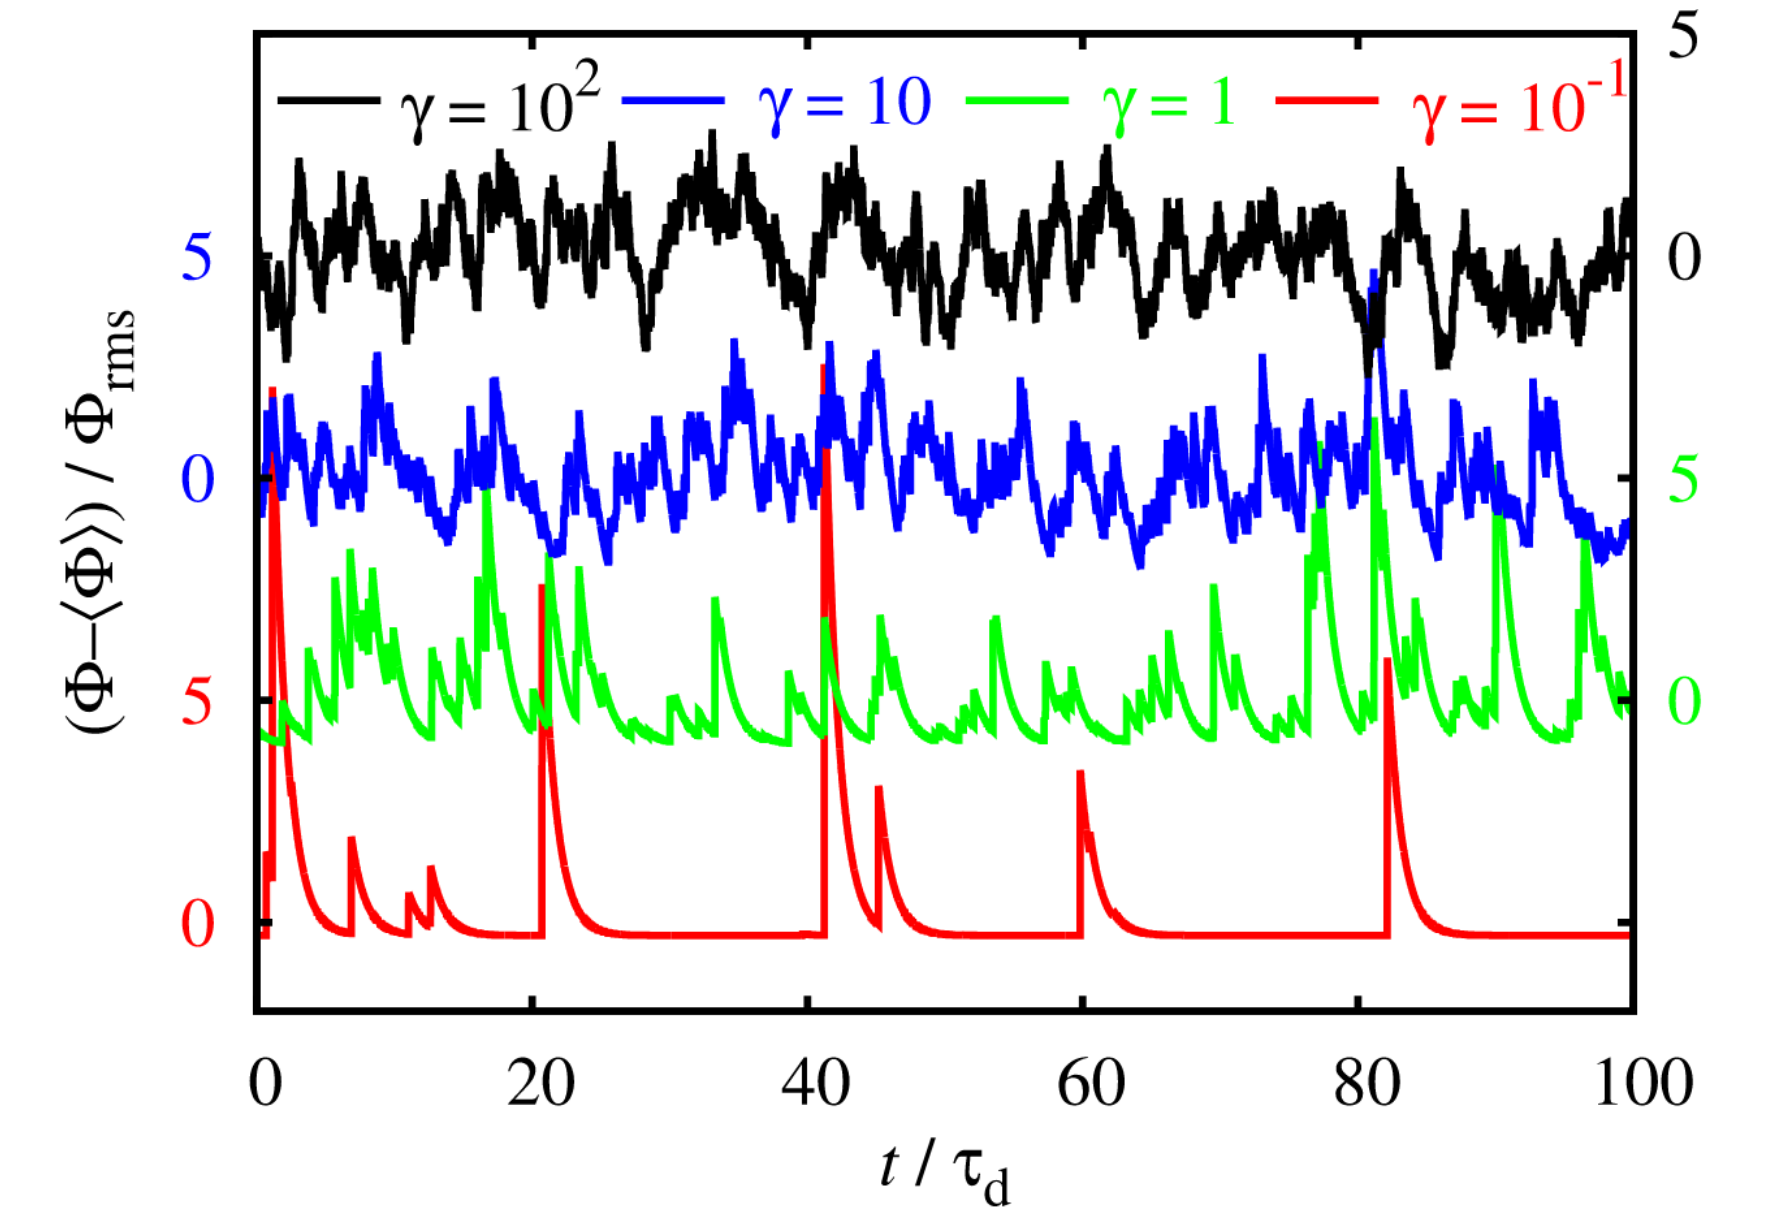
\includegraphics[width=\linewidth]{figures/garcia_realizations.png}
% 		\caption{Realizations of the FPP with one-sided exponential pulses and different intermittency parameters. Reprinted from \cite{garcia2016stochastic}, with the permission from AIP Publishing.}
% 		\label{Fig:garcia_realizations}
% 	\end{minipage}
% 	\hfill
% 	\begin{minipage}{.48\linewidth}
% 		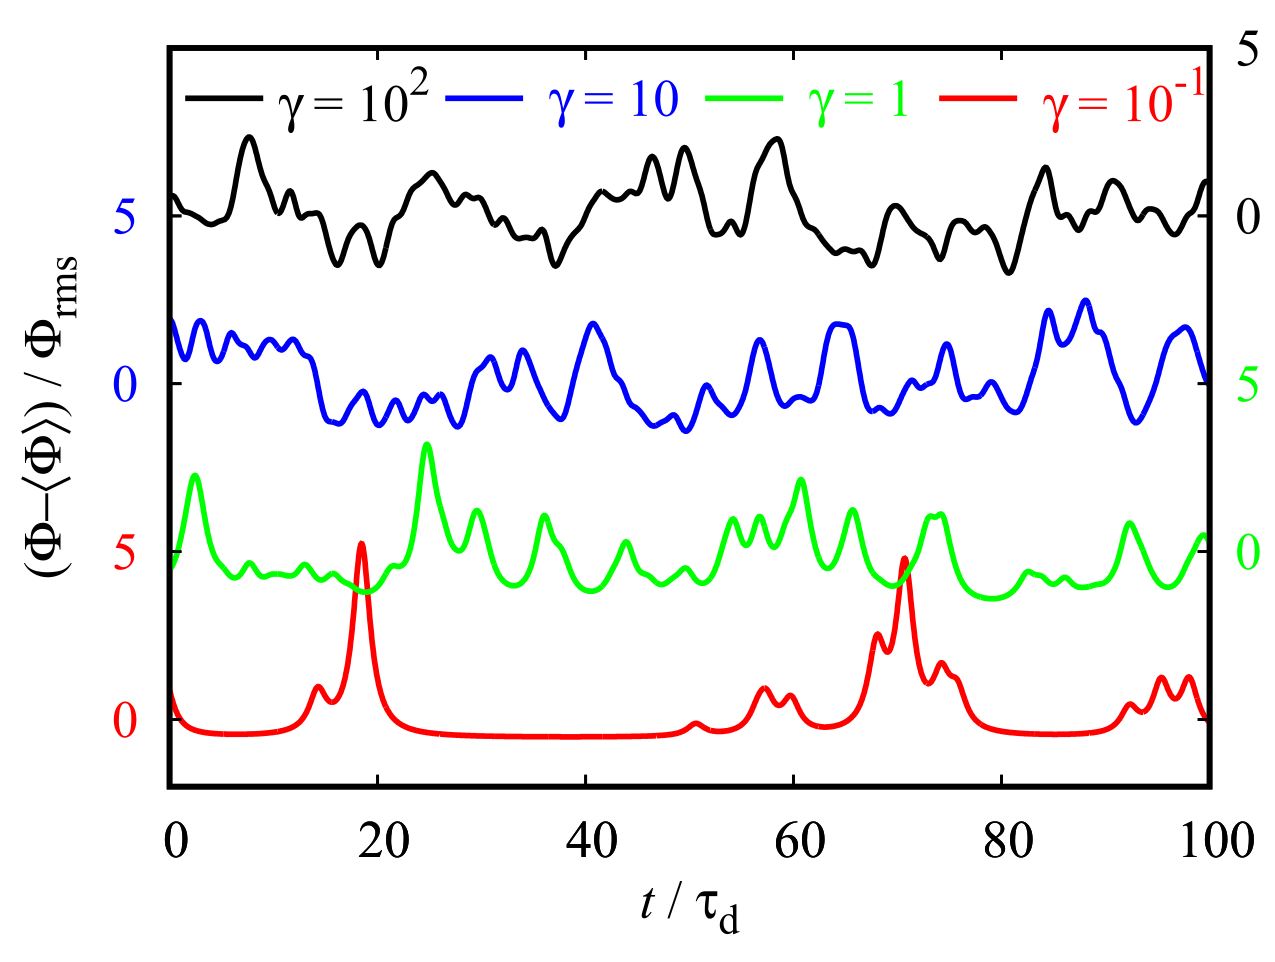
\includegraphics[width=\linewidth]{figures/garcia_lorentz.png}
% 		\caption{Realizations of the FPP with Lorentzian pulses and different intermittency parameters. Reprinted from \cite{garcia2017power}, with the permission from AIP Publishing.}
% 		\label{Fig:garcia_realizations_lorentz}
% 	\end{minipage}
% \end{figure}

% \section{Moments and PDFs}
% The four lowest order central moments of the FPP take the form 
% \begin{subequations}
% 	\begin{align}
% 		\langle\Phi\rangle  &= \gamma \langle A \rangle I_1,\\
% 		\Phi^2_\mathrm{rms} &= \gamma \langle A^2\rangle I_2,\\
% 		S_\Phi &= \frac{1}{\gamma^{1/2}}\frac{\langle A^3\rangle I_3}{\langle A^2\rangle^{3/2} I_2^{3/2} },\\
% 		F_\Phi &= 3 + \frac{1}{\gamma} \frac{\langle A^4\rangle I_4}{\langle A^2\rangle^2 I_2^2}, 
% 	\end{align}
% \end{subequations}
% where $S_\Phi$ stands for the skewness of the process and $F_\Phi$ is the kurtosis or flatness \cite{garcia2012stochastic}. The last two moments exhibit the parabolic relationship 
% \begin{equation}\label{parabolic}
% 	F_\Phi = 3 + \frac{\langle A^2\rangle \langle A^4\rangle}{\langle A^3\rangle^2}\frac{I_2 I_4}{I^2_3} S_\Phi^2.
% \end{equation}
% Inserting the expressions for the integrals of the pulse shapes for two-sided exponential and Lorentzian pulses and assuming exponentially distributed amplitudes simplifies these expressions further. For exponential pulses the expression for the relative fluctuation level becomes
% \begin{equation}
% 	\frac{\Phi_{\mathrm{rms}}}{\langle \Phi\rangle} = \gamma^{-1/2},
% \end{equation}
% and the universal parabolic relationship of \Eqref{parabolic} reduces to
% \begin{equation}
% 	F_\Phi = 3 + \frac{3}{2} S_\Phi^2,
% \end{equation} 
% which stands in good agreement with experimental measurements \cite{labit2007universal,sattin2009statistics,sattin2009parabolic}. Notably, these expressions do not depend on the pulse asymmetry parameter, $\lambda$. 

% The PDF of the process with exponential pulses is given by a Gamma distribution with shape parameter $\gamma$ and scale parameter $\langle A \rangle$ \cite{theodorsen2018probability},

% \begin{equation}
% 	P_{\Phi,\phi}(\Phi) = \frac{\Phi^{\gamma-1}}{\langle A\rangle^\gamma \Gamma(\gamma)}\mathrm{exp}\left(-\frac{\Phi}{\langle A\rangle}\right).
% \end{equation}
% Typically, the realization of the process is normalized to have zero mean and unit standard deviation,
% \begin{equation}\label{norm}
% 	\widetilde{\Phi} = \frac{\Phi - \langle\Phi\rangle}{\Phi_{\mathrm{rms}}},
% \end{equation}
% with the according PDF \cite{theodorsen2018probability},
% \begin{equation}
% 	P_{\widetilde{\Phi},\phi}(\widetilde{\Phi}) = \frac{\gamma^{\gamma/2}}{\Gamma(\gamma)}\left(\widetilde{\Phi} + \gamma^{1/2} \right)^{\gamma-1}\mathrm{exp}\left(-\gamma^{1/2}\widetilde{\Phi} - \gamma\right).
% \end{equation}
% This expression is used as a fit in \Figref{Fig:theodorsen_pdf}. For an FPP of Lorentzian pulses no closed expressions for its PDF is known. However, it can be derived by taking the inverse Fourier transform of its corresponding characteristic function resulting in \cite{garcia2018lorentz}
% \begin{equation}
% 	\begin{split}
% 	P_{\widetilde{\Phi},\psi}(\widetilde{\Phi}) = \left(\frac{\pi}{\gamma}\right)^{1/2}\int_{0}^{\infty}\textrm{d}w\,\mathrm{exp}\left(-\frac{\gamma\pi w\, \mathrm{sin}\left(1/2\, \mathrm{arctan}\, w\right)}{(1+w^2)^{1/4}}\right)\\
% 	\times \mathrm{cos}\left(\pi\gamma w + \sqrt{\pi\gamma}\widetilde{\Phi}w-\frac{\gamma\pi w\, \mathrm{cos}\left(1/2\, \mathrm{arctan}\, w\right)}{(1+w^2)^{1/4}}\right).
% 	\end{split}
% \end{equation}
% For both exponential and Lorentzian pulses the PDF of the processes are characterized by the intermittency parameter. The PDFs are shown for a range of different $\gamma$ in \Figref{Fig:garcia_pdf} and \Figref{Fig:garcia_pdf_lorentz}. The PDFs are unimodal for all values of $\gamma$ and have an exponential tail towards large fluctuation amplitudes for small values of $\gamma$. In the opposite limit, the PDFs approach a normal distribution with vanishing mean and unit standard deviation for $\widetilde{\Phi}$.

% \begin{figure}
% 	\centering
% 	\begin{minipage}{.48\linewidth}
% 		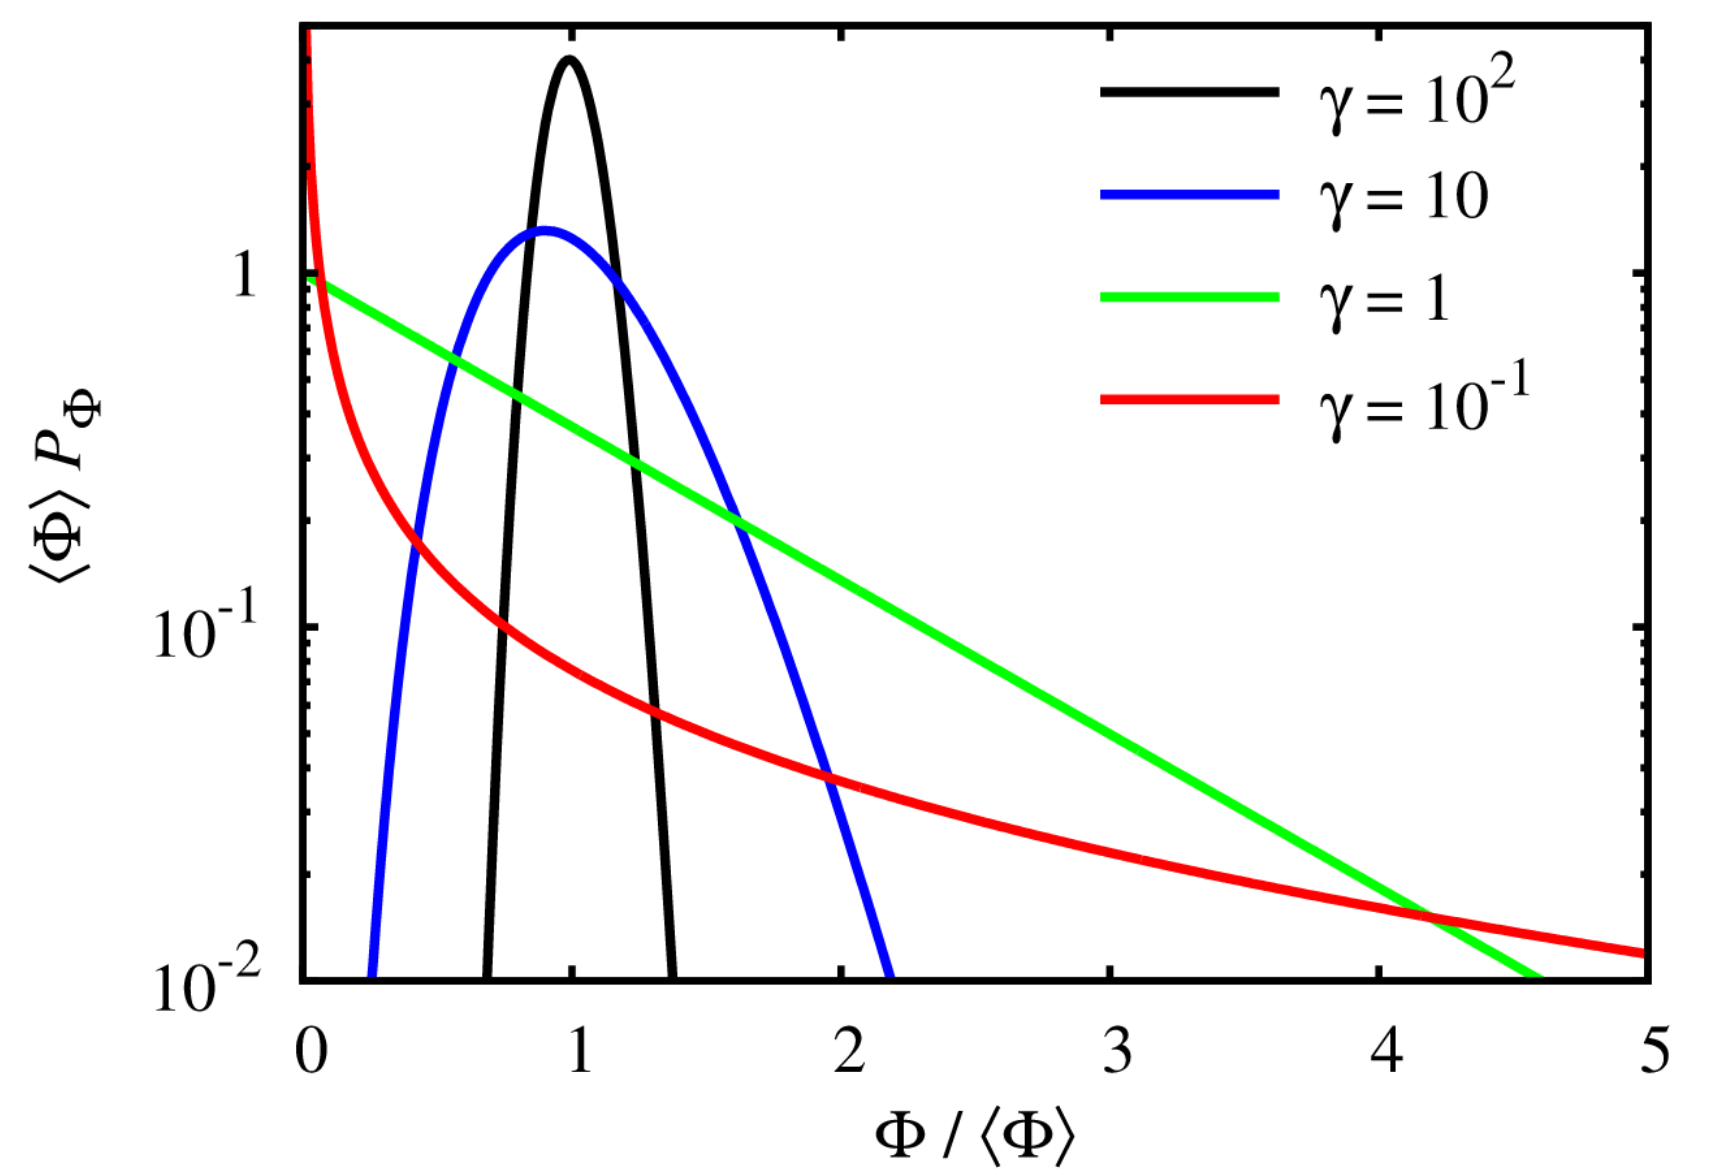
\includegraphics[width=\linewidth]{figures/garcia_pdf.png}
% 		\caption{PDFs of a FPP with exponential pulses with different intermittency parameters $\gamma$. Reprinted from \cite{garcia2016stochastic}, with the permission from AIP Publishing.}
% 		\label{Fig:garcia_pdf}
% 	\end{minipage}
% 	\hfill
% 	\begin{minipage}{.48\linewidth}
% 		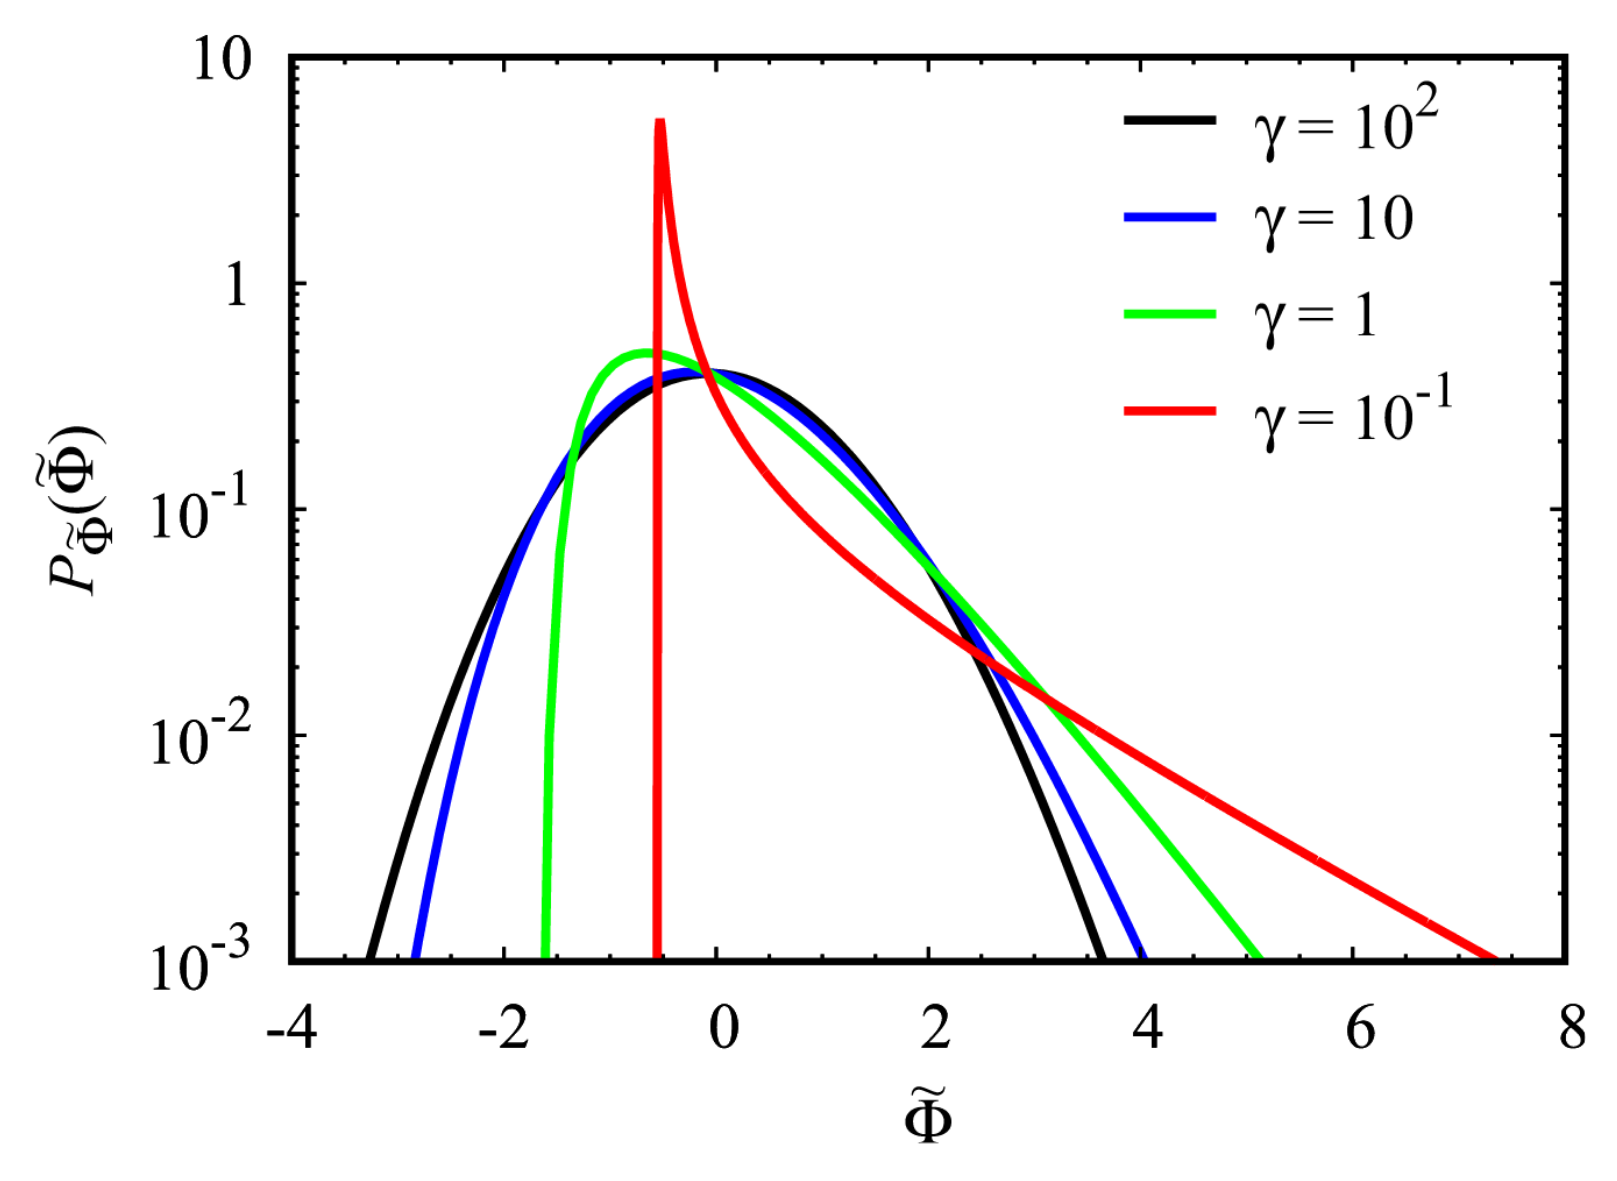
\includegraphics[width=\linewidth]{figures/garcia_pdf_lorentz.png}
% 		\caption{PDFs of a normalized FPP with Lorentzian pulses with different intermittency parameters $\gamma$. Reprinted from \cite{garcia2018lorentz}, with the permission from AIP Publishing.}
% 		\label{Fig:garcia_pdf_lorentz}
% 	\end{minipage}
% \end{figure}
% \section{Second order statistics}

% In order to calculate the second order moments, namely the power spectral density (PSD) and the Auto-correlation function (ACF), we consider the FPP as a convolution of a pulse train $f_K$ and a pulse shape $\phi$. The Fourier transform of the FPP is given by the product of the Fourier transform of $f_K$ and $\phi$. The power spectrum of $\Phi$ can therefore be expressed as the product of the power spectrum of $f_K$ and $\phi$. The power spectrum of $f_K$ is flat due to the uncorrelated delta pulses, so that the frequency dependence of the spectrum of $\Phi$ is only dependent on $\phi$. The ACF is given by the Fourier transform of the PSD. For two-sided exponential pulses the PSD of an FPP normalized according to \Eqref{norm}, takes the form \cite{garcia2017auto}
% \begin{equation}
% 	\Omega_{\widetilde{\Phi},\phi}(\omega;\lambda) = \frac{2 \tau_\mathrm{d}}{[1+(1-\lambda)^2\tau_\mathrm{d}^2\omega^2][1+\lambda^2\tau_\mathrm{d}^2\omega^2]},
% \end{equation}
% with the according ACF
% \begin{equation}
% 	R_{\widetilde{\Phi},\phi}(r;\lambda) = \frac{1}{1-2\lambda}\left[\left(1-\lambda\right)\mathrm{exp}\left(-\frac{|r|}{(1-\lambda)\tau_\mathrm{d}}\right) -\lambda\,\mathrm{exp}\left(-\frac{|r|}{\lambda\tau_\mathrm{d}}\right)\right].
% \end{equation}
% The ACF and PSD are displayed for a range of $\gamma$-values in \Figsref{Fig:garcia_acf} and \ref{Fig:garcia_psd}.
% \begin{figure}
% 	\centering
% 	\begin{minipage}{.48\linewidth}
% 		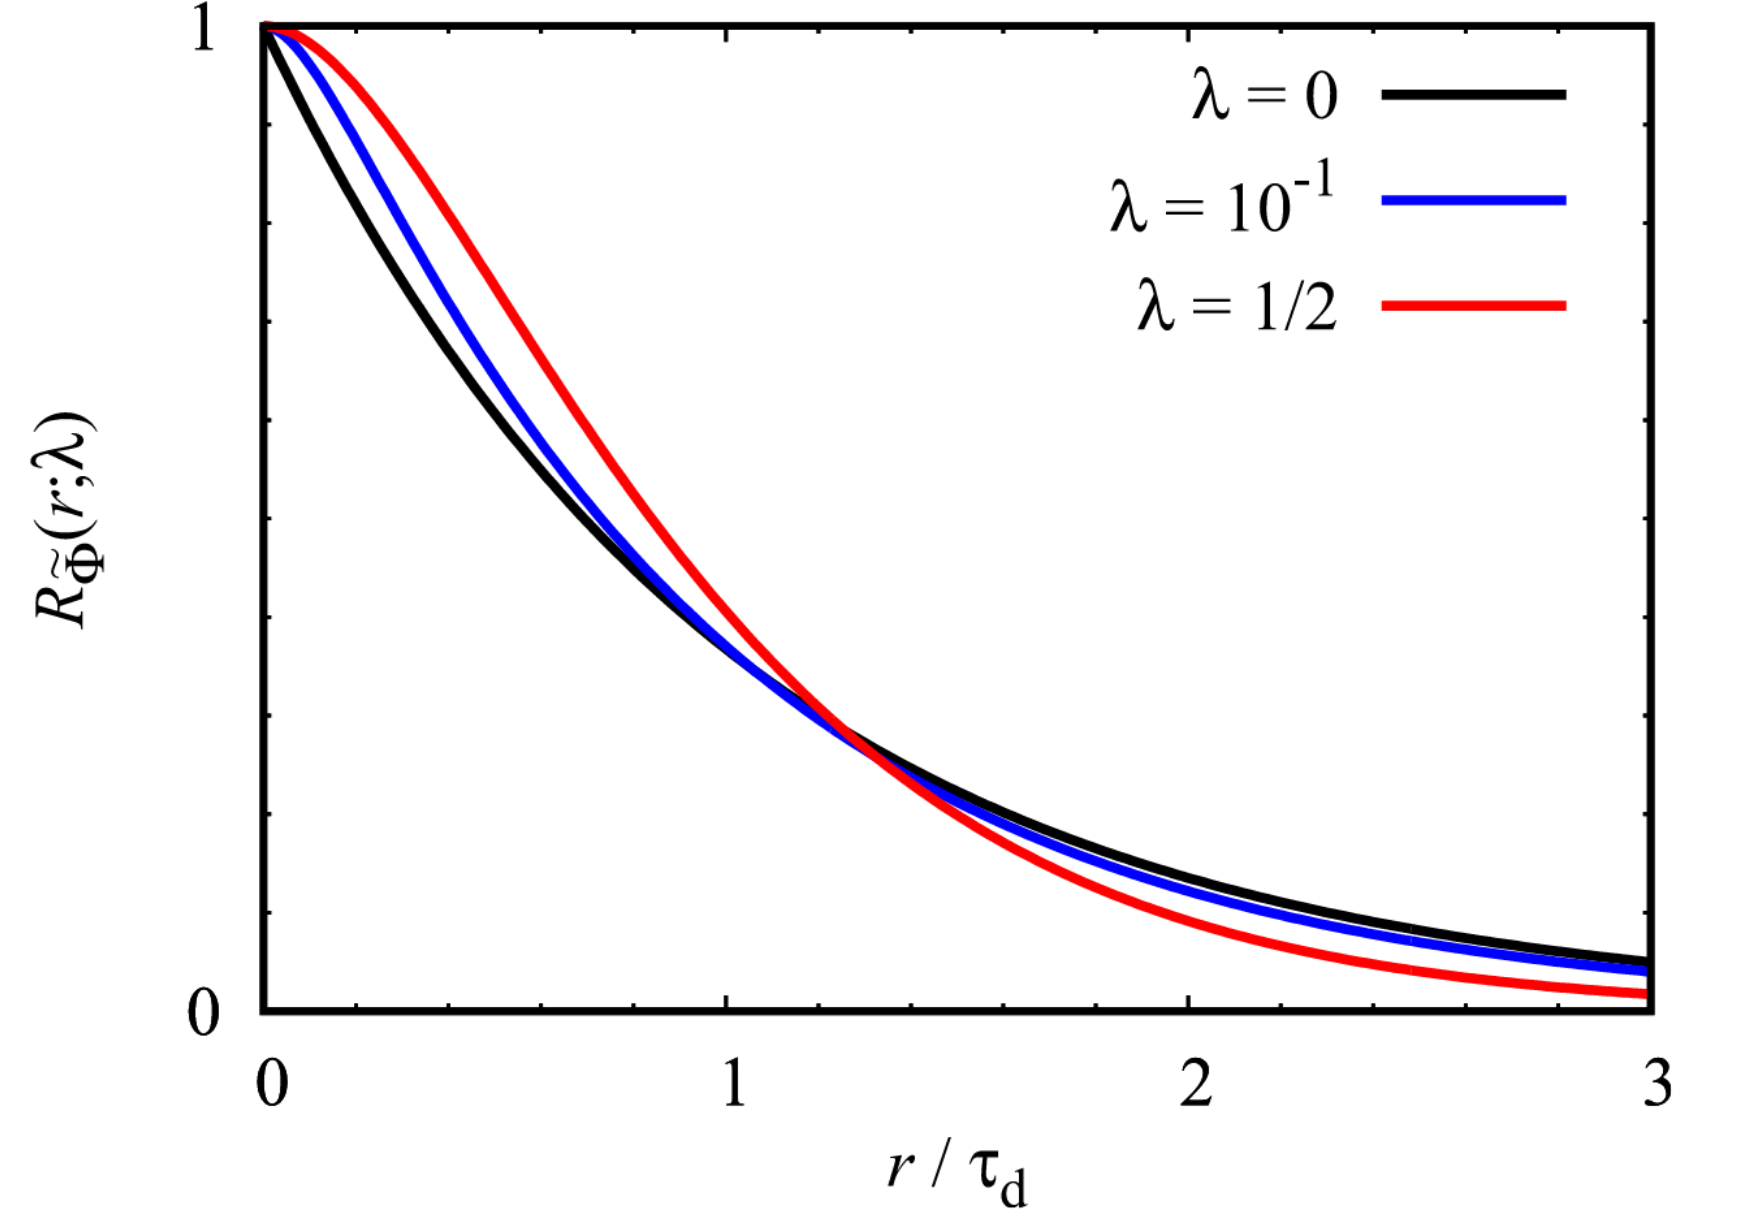
\includegraphics[width=\linewidth]{figures/garcia_acf.png}
% 		\caption{Auto-correlation function of a normalized FPP consisting of two-sided exponential pulses with different asymmetry parameters $\lambda$. Reprinted from \cite{garcia2017auto}, with the permission from AIP Publishing.}
% 		\label{Fig:garcia_acf}
% 	\end{minipage}
% 	\hfill
% 	\begin{minipage}{.48\linewidth}
% 		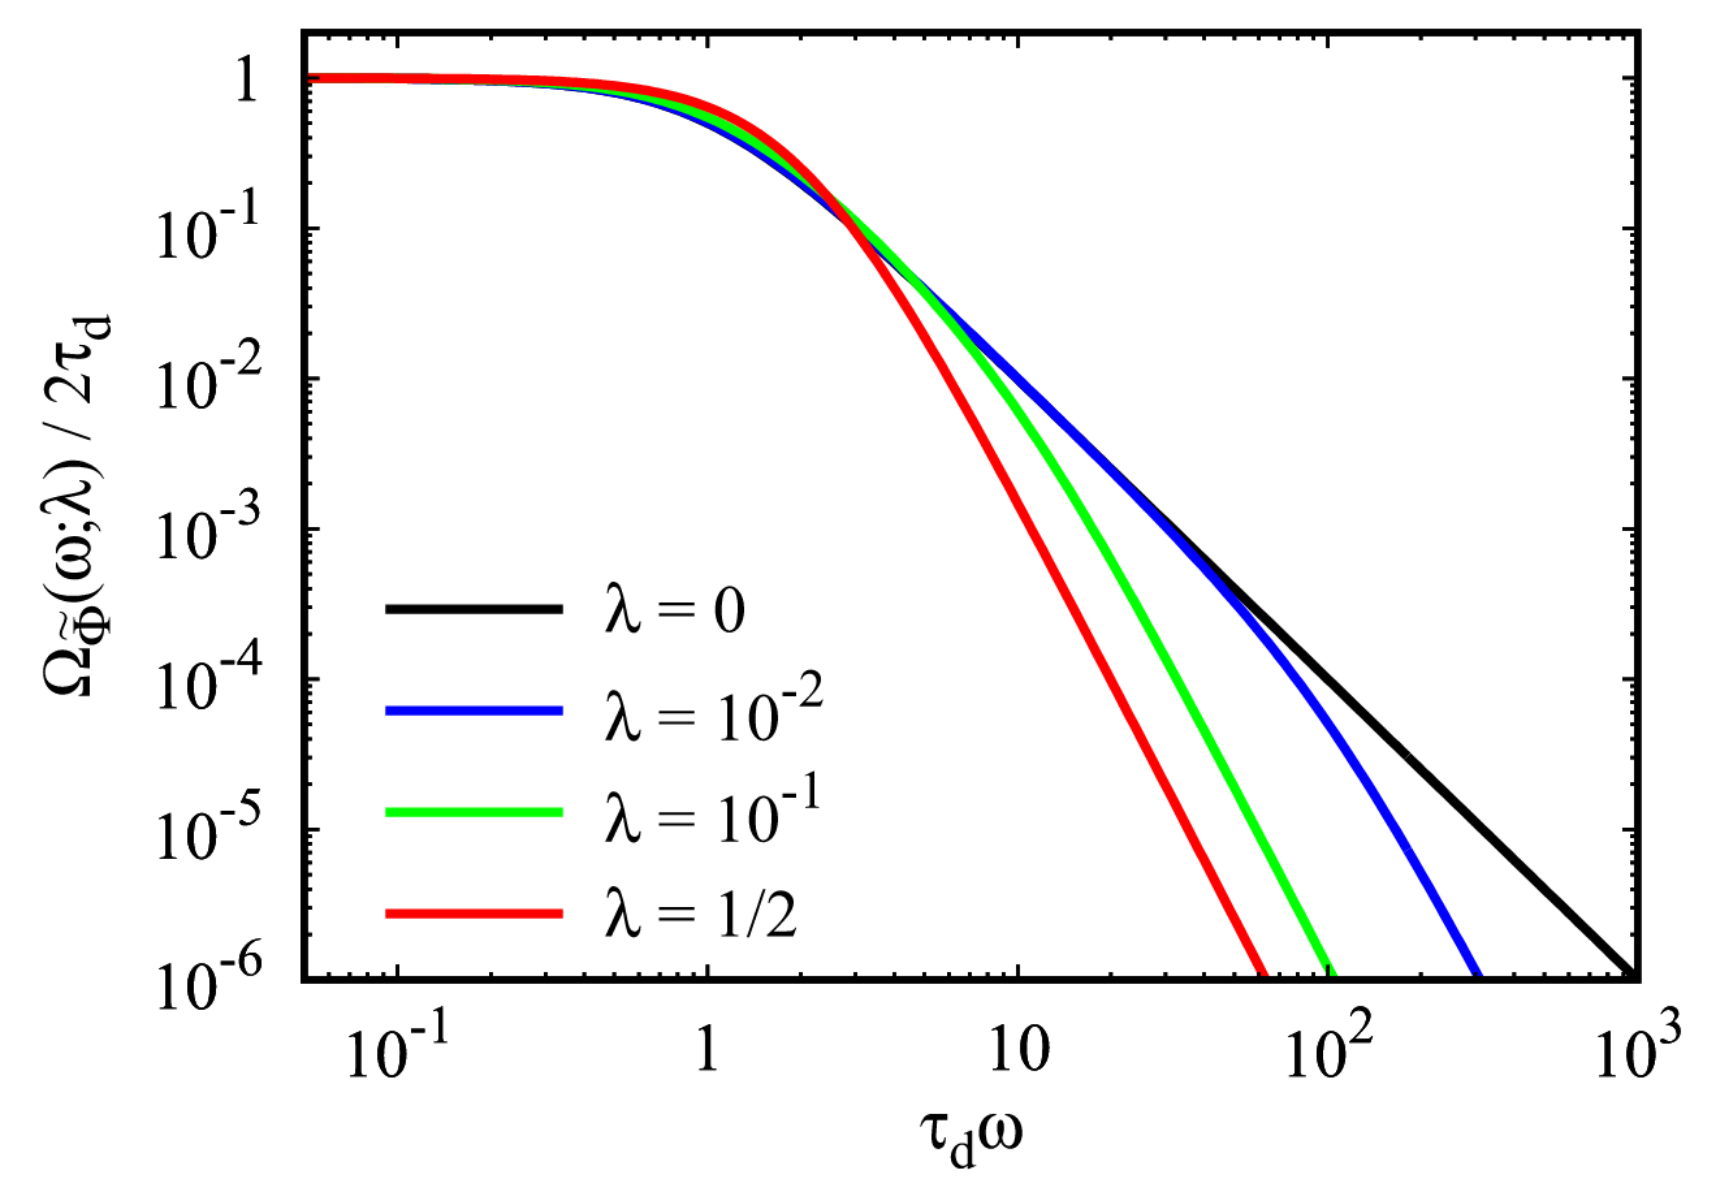
\includegraphics[width=\linewidth]{figures/garcia_psd.png}
% 		\caption{Power spectral density of a normalized FPP consisting of two-sided exponential pulses with different asymmetry parameters $\lambda$. Reprinted from \cite{garcia2017auto}, with the permission from AIP Publishing.}
% 		\label{Fig:garcia_psd}
% 	\end{minipage}
% \end{figure}
% In contrast to the PDFs, the second order statistics are independent of $\gamma$ but change for different $\lambda$. In the limits of a one-sided exponential pulse, the ACF is purely exponential and the PSD is Lorentzian shaped. For $\lambda$ close to zero or 1, the spectrum has an intermediate range where the spectrum falls with $\omega^{-2}$ before it falls with $\omega^{-4}$ in the high frequency limit. This expression is in excellent agreement with the experimental measurements shown in \Figref{Fig:theodorsen_psd} with $\lambda=0.1$. 

% For Lorentzian pulses the PSD of a normalized FPP takes an exponential form \cite{garcia2018skewed}
% \begin{equation}
% 	\Omega_{\widetilde{\Phi},\psi}(\omega) = 2\pi\tau_\mathrm{d}\, \mathrm{exp}\left(-2\tau_\mathrm{d}|\omega|\right),
% \end{equation}
% and the ACF is Lorentzian shaped,
% \begin{equation}
% 	R_{\widetilde{\Phi},\psi}(r) = \frac{4}{4+(r/\tau_\mathrm{d})^2}.
% \end{equation}
% These expressions can be generalized to skewed Lorentzian pulses, however no closed expressions are known. An alternative formulation is presented in \cite{garcia2018skewed}.

% \section{Excess time statistics}
% Expressions for excess time statistics, specifically the rate of level crossings above a given threshold and the average time spent above this threshold, can be derived for an FPP. In the context of fluctuations in the SOL of fusion experiments, these quantities are crucial considering the energy of incoming particles to the vessel walls and the energy threshold of physical sputtering. The number of sputtered particles per incoming particle is specified by the modified Bohdansky yield function \cite{marandet2016assessment}. The mean yield as a function of energy of an incoming deuterium particle on a tungsten wall is plotted for a range of relative fluctuation levels in \Figref{Fig:theodorsen_yield}. For constant energy, no sputtering occurs beneath 200 eV. For realistic scenarios of $E_\mathrm{rms}/\langle E\rangle > 0$ sputtering already occurs at significantly lower mean energies. An accurate description of excess time statistics is therefore of importance for fusion experiments. 

% For an FPP the number of level crossings is given by Rice's formula \cite{rice1945mathematical}
% \begin{equation}
% 	X(\Phi) = T\int_{0}^{\infty} \mathrm{d}\dot{\Phi}\, \dot{\Phi}P_{\Phi,\dot{\Phi}}\left(\Phi,\dot{\Phi}\right).
% \end{equation}
% Here $\dot{\Phi}$ stands for the derivative of the process $\Phi$ and $P_{\Phi,\dot{\Phi}}\left(\Phi,\dot{\Phi}\right)$ for the joint PDF between $\Phi$ and $\dot{\Phi}$. This formulation requires the process to be differentiable, hence an FPP consisting of one-sided exponential pulses cannot be considered this way. For two-sided exponential pulses with $\lambda \in (0,1)$ the rate of up-crossings is given by \cite{theodorsen2018level}
% \begin{equation}\label{rate}
% 	\frac{\tau_\mathrm{d}}{T}X(\Phi) = \frac{\lambda^{\gamma\lambda-1}(1-\lambda)^{\gamma(1-\lambda)-1}}{\gamma\Gamma(\gamma\lambda)\Gamma(\gamma(1-\lambda))}\left(\frac{\gamma\Phi}{\langle\Phi\rangle}\right)^\gamma\mathrm{exp}\left(-\frac{\gamma\Phi}{\langle\Phi\rangle}\right).
% \end{equation}
% For this expression, the limit $\lambda\rightarrow0$ exists. \Eqref{rate} is plotted for exponential pulses with $\lambda=0$ and $\lambda=1/2$ and a range of $\gamma$-values in \Figref{Fig:theodorsen_avtime}. From this, the PDF of time as well as mass above a given threshold can be determined analytically for the limits $\gamma\rightarrow 0$ and $\gamma\rightarrow \infty$  and numerically with Monte Carlo simulations for general $\gamma$ \cite{theodorsen2018level}. 
% \begin{figure}
% 	\centering
% 	\begin{minipage}{.48\linewidth}
% 		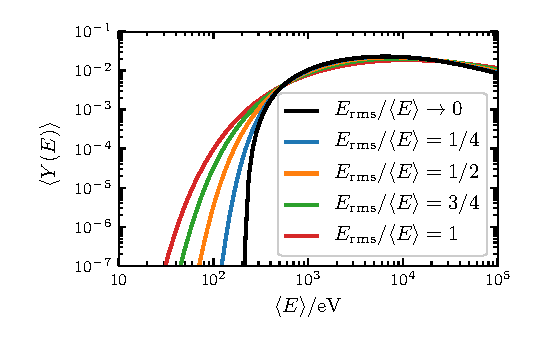
\includegraphics[width=\linewidth]{figures/yield_fun_mE_W.eps}
% 		\caption{Mean yield  function for a range of relative fluctuation levels. Image courtesy of A. Theodorsen \cite{theodorsen2018statistical}.}
% 		\label{Fig:theodorsen_yield}
% 	\end{minipage}
% 	\hfill
% 	\begin{minipage}{.48\linewidth}
% 		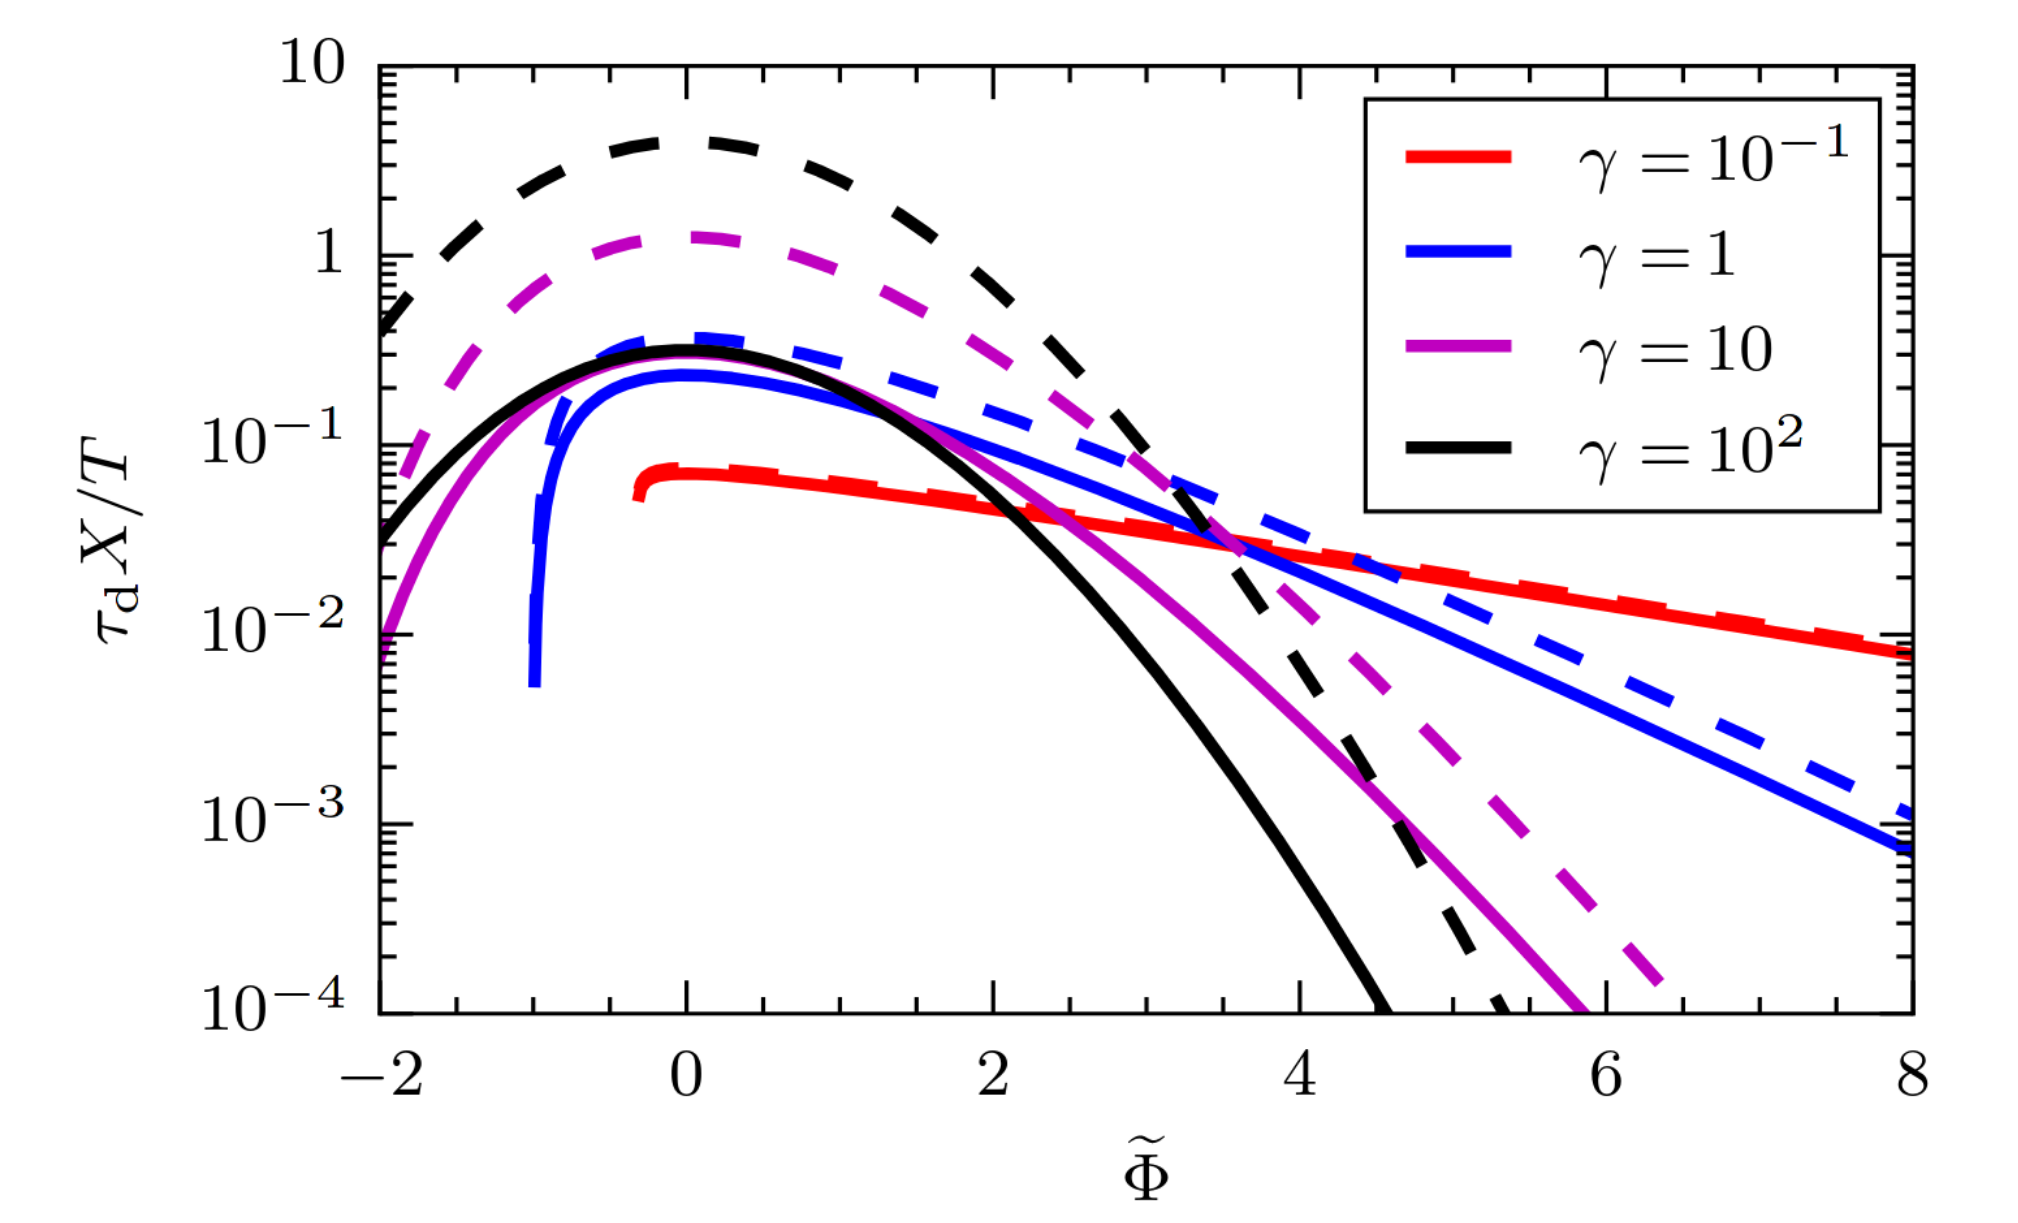
\includegraphics[width=\linewidth]{figures/theodorsen_rate.png}
% 		\caption{Rate of up-crossings for a FPP consisting of exponential pulses with $\lambda=0$ (dashed line) and $\lambda=1/2$ (full line) for various $\gamma$-values. Reprinted figure with permission from \cite{theodorsen2018level}. Copyright (2018) by the American Physical Society.}
% 		\label{Fig:theodorsen_avtime}
% 	\end{minipage}
% \end{figure}

% At the time of writing this thesis, excess time statistics of an FPP consisting of Lorentzian pulses have not been investigated.

% \section{Density profiles}\label{n_prof}
% The FPP can be extended to include a spatial variable $x$, resulting in a model of advecting single pulses and corresponding profiles. In the following, this model is discussed in the context of filament motion in SOL plasmas. The presented notation is consistent with \cite{garcia2016stochastic}. Alternative formulations based on a Lagrangian approach to filament dynamics result in equivalent expressions \cite{militello2016scrape,militello2016relation,walkden2017interpretation,militello2018two}.

% The model is given by a superposition of pulses 
% \begin{equation}
% 	\Phi_K(x,t) = \sum_{k=1}^{K} \phi_k(x,t).
% \end{equation}
% In contrast to previous sections $\phi_k$ is compounded by both amplitude and pulse shape. For simplicity, we keep $K$ constant in the following derivation. The evolution of individual pulses, neglecting pulse interaction, is given by the modified advection equation,
% \begin{equation}\label{phi_equation}
% 	\frac{\partial \phi_k}{\partial t} + v_\perp\frac{\partial \phi_k}{\partial x} + \frac{\phi_k}{\tau_\parallel} = 0,
% \end{equation}
% with $v_\perp$ as the radial velocity and $\tau_\parallel$ representing the parallel transit time, describing parallel losses along the magnetic field. Note, that we assume $v_\perp$ and $\tau_\parallel$ to be constant for all filaments. Following \Eqref{phi_equation}, individual pulses can be written as the product of their amplitude and pulse shape, $	\phi_k(x,t) = A_k(t)\varphi_k(x-x_k-v_k t)$ with $x_k$ as the position of the pulse at $t=0$. The individual amplitudes are assumed to satisfy the expression 
% \begin{equation}
% 	\frac{\mathrm{d}A_k}{\mathrm{d}t} = -\frac{A_k}{\tau_\parallel}.
% \end{equation}
% The solution for this amplitude equation can be expressed by introducing the initial amplitude $A_{0k}$ resulting in
% \begin{equation}
% 	A_k(t) = A_{0k}\,\mathrm{exp}\left(-\frac{t+x_k/v_\perp}{\tau_\parallel}\right),
% \end{equation}
% with the pulse $k$ being located at $x=0$ at time $-x_k/v_\perp$. We further assume the pulse shape to take the form of an exponential function,
% \begin{equation}
% 	\varphi_k(x) = \Theta\left(-\frac{x}{l_\perp}\right)\mathrm{exp}\left(\frac{x}{l_\perp}\right),
% \end{equation}
% where $\Theta$ is the Heaviside function and $l_\perp$ is the radial size of the pulse. Note, that this pulse shape is consistent with the findings shown in \Figref{Fig:garcia_1}. We now consider the signal at a reference position $\xi$. At the reference time $t_k = (\xi - x_k)/v_\perp$ for pulse $k$ at position $\xi$, the process takes the form
% \begin{equation}
% 	\Phi_K(\xi, t) = \sum_{k=1}^{K}A_{0k}\,\mathrm{exp}\left(-\frac{\xi}{v_\perp \tau_\parallel}\right)\Theta\left(\frac{t-t_k}{\tau_\perp}\right)\exp\left(-\frac{t-t_k}{\tau_\mathrm{d}}\right),
% \end{equation}
% with $\tau_\perp = l_\perp/v_\perp$ and the pulse duration given by the harmonic mean of the perpendicular and parallel transit time $\tau_\mathrm{d} = \tau_\parallel\tau_\perp/(\tau_\parallel+\tau_\perp)$. By averaging over uniformly distributed pulse arrivals, the resulting radial profile takes the exponential form
% \begin{equation}
% 	\langle\Phi\rangle(\xi) = \frac{\tau_\mathrm{d}}{\tau_w}\langle A_0\rangle\mathrm{exp}\left(-\frac{\xi}{v_\perp\tau_\parallel}\right).
% \end{equation}
% The resulting scale length of the profile is governed by the radial velocity of the filaments and the parallel transit time. Multiple realizations at individual points in time and the corresponding mean profile are shown in \Figref{Fig:militello}. 

% The application of this model exhibits numerous limitations. The assumption of constant radial velocities and pulse size is an overly simplified description for filament transport in the SOL. In addition, the assumption of radially constant $\tau_w$ and therefore radially constant $\gamma$ does not hold in experimental observations. Interactions between individual filaments and two-dimensional motion are also not considered. However, this mathematical model still provides valuable insight in the relation between individual filaments and radial profiles in the SOL and can serve as a framework to relate isolated blob and filament studies to turbulence simulations and experimental measurements. 

% \begin{figure}[t]
% 	\centering
% 	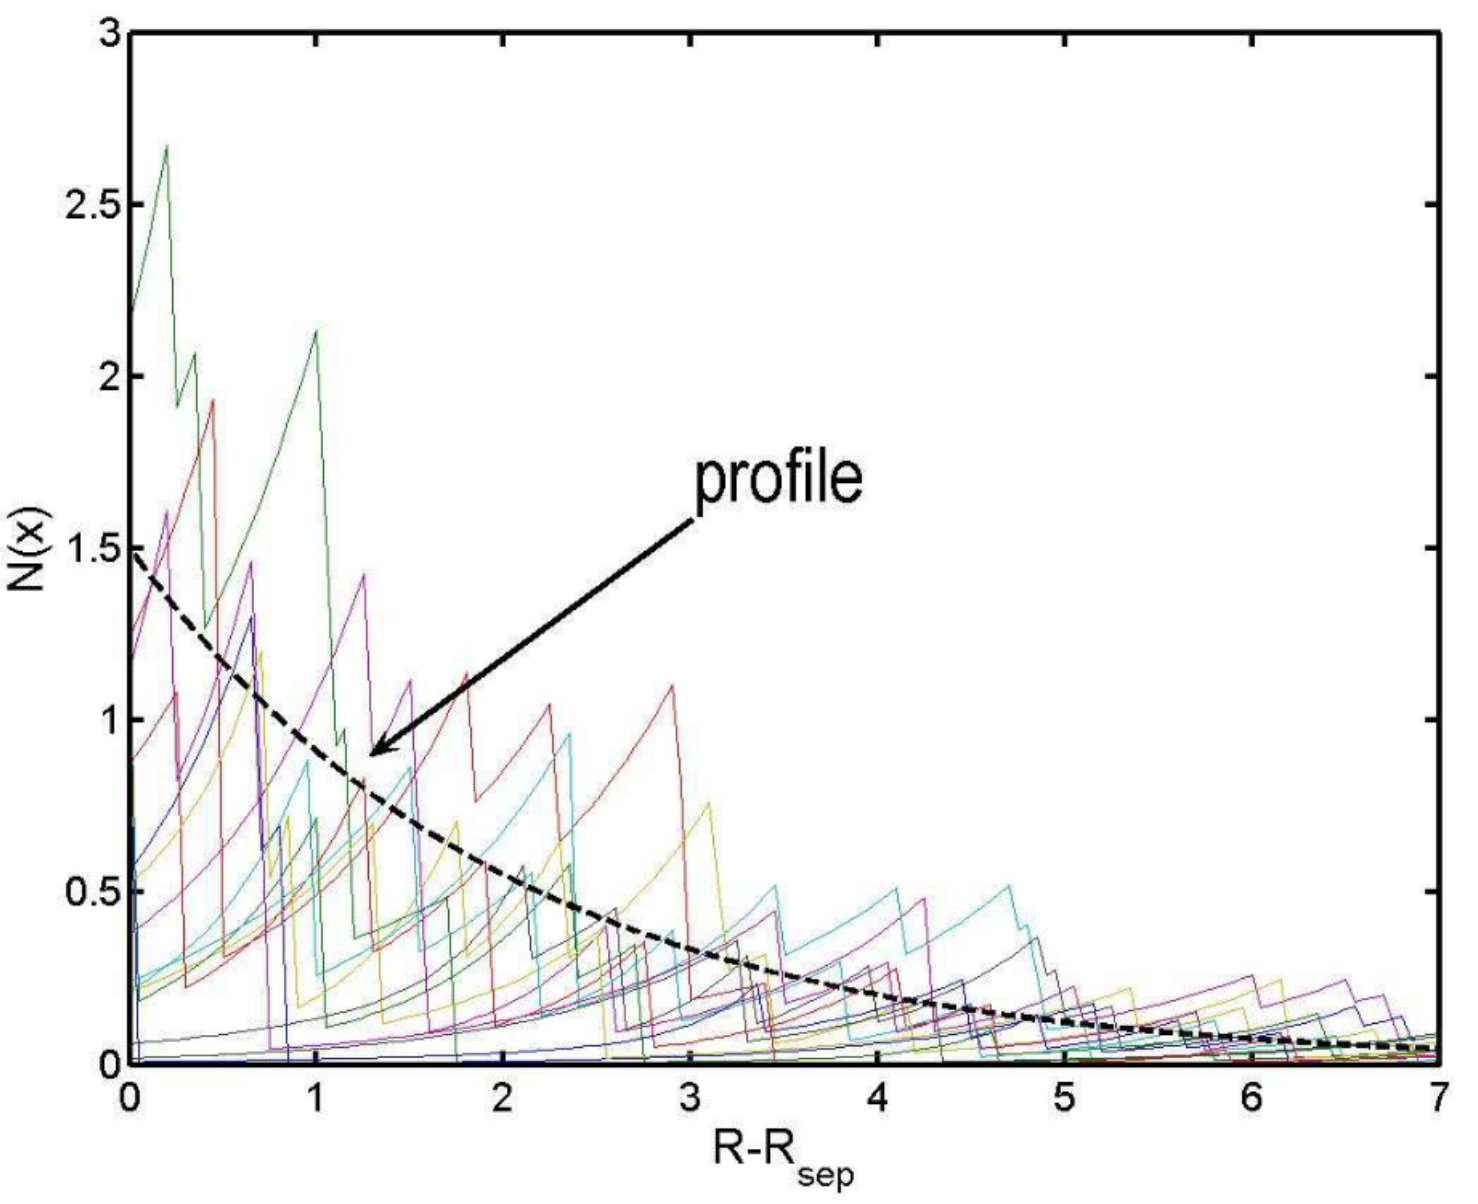
\includegraphics[width=9cm]{figures/militello_profile.png}
% 	\caption{Radial exponential density profile (black dashed line) illustrated as the mean of individual density realizations (colored lines) given by a superposition of individual exponentially shaped pulses. Image courtesy of F. Militello \cite{militello_profiles}.}
% 	\label{Fig:militello}
% \end{figure}
% \section{Deconvolution method}
% Since the FPP can be expressed as a convolution of a pulse function $\phi$ and a forcing, consisting of delta-function pulses $f_K$, shown in \Eqref{conv}, one can attempt to estimate the forcing if the pulse shape is known \cite{theodorsen2018universality, decristoforo2020intermittent, kube2020comparison}. For a given forcing, one can determine the pulse amplitudes $\{ A_k \}_{k=1}^K$ and arrival times $\{ t_k \}_{k=1}^K$ directly. This method has the advantage of capturing pulses of all sizes, not only events above a certain threshold as is the case for conditional averaging. Additionally, the problem of pulse overlap is less severe. In order to estimate the forcing, a modified Richardson-Lucy deconvolution algorithm can be used \cite{richardson1972bayesian,lucy1974iterative}. The algorithm is initialized with a first guess for the forcing $f_K^{(1)}$. This value is iteratively updated with the $n$-th iteration given by
% \begin{equation}
% 	f_K^{(n+1)} = f_K^{(n)} \frac{D*\widehat{\phi}}{f_K^{(n)}*\phi*\widehat{\phi}}.
% \end{equation}
% Here, $\widehat{\phi}(t) = \phi(-t)$ and $D$ denotes the investigated time series. This algorithm converges to the least squares solution \cite{dell2007model}. The initial guess for the forcing matters little as it only determines the number of iterations required until the algorithm converges. 

% This deconvolution algorithm thereby provides a versatile tool to analyze time series of SOL fluctuations in experiments and simulations, as it can provide clear results even for relatively short time series.   




\chapter{Summary of Papers}\label{ch:sum-paper}
The~thesis aims to infer physical properties of the~interplanetary dust in terms of dust populations by analyzing experimental data. We use the~electrical antenna measurements of two spacecraft: SolO and PSP. To yield the~most information, the~data had to be treated carefully, keeping the~limited confidence of dust identification in mind. The~dust cloud analysis is indirect, as the~antenna measurements yield little information about each individual impact. Therefore, the~physical properties of the~dust populations only emerge in statistics. 

The~main body of this work is the~four papers presented below. Each of the~papers has several co-authors, and the~thesis author's particular contribution is explicitly described in the~acknowledgments in each of the~papers.

\subsubsection{Paper~I}

SolO's antennas record electrical time-domain waveforms when the~electric field shows signs of potentially interesting activity, not necessarily of dust origin. It is a~long-standing issue to convincingly classify electrical signatures by means other than visual event-by-event human labelling. In Paper~I, we report on the~development of a~machine learning tool, which provides this functionality. We tried two machine learning approaches and improvement was attained with a~purpose-developed convolutional neural network, which achieved $\SI{96}{\%}$ classification accuracy and $\SI{94}{\%}$ precision, compared to $\SI{85}{\%}$ accuracy and $\SI{75}{\%}$ precision of the~previously used algorithm. Developing this tool was instrumental for the~future work on SolO dust counts, as a~solid data product was key for any more refined analysis, such as that done in Papers II and III. 

\subsubsection{Paper~II}

There are many degrees of freedom in dust flux models. To constrain them as much as possible, we employed a~Bayesian approach to analyze the~antenna dust counts for the~first time in Paper~II. We constructed a~semi-empirical two-component model, inspired by previous works of other authors, and applied it on SolO data, specifically the~data product of Paper~I, from between 07/2020 and 12/2021, all recorded between $\SI{0.5}{AU}$ and $\SI{1}{AU}$. We estimated the~speed of outgoing $\beta$-meteoroids to $63 \pm 7 \, \si{kms^{-1}}$. We found with confidence that the~$\beta$-meteoroid population is decelerating on its way out of the~inner solar system, which clearly implies that the~radiation pressure is lower than gravity for these grains, that is $\beta < 1$. 

\subsubsection{Paper~III}

In Paper~II, we only used the~impact counts, that is the~binary information, whether an impact happened, for each of the~many temporal intervals. Electrical antenna measurements also provide information about the~amplitude and shape of each of the~impacts, which was disregarded in Paper~II. This was the~motivation for Paper~III, where we report on the~finding that the~signals recorded with SolO/RPW are typically double peaked. In fact, we found that the~chronologically first peak, denoted \textit{primary}, is explainable by the~current theory of the~dust impact signal formation. The~\textit{secondary} peak, which was found to be much more variable, was found to appear on a~significantly longer time scale explained by the~ion motion. This is possibly explained by the~escaping ions having influence on the~individual antennas. We found this secondary peak to be too strong for direct ion detection. A~possible explanation was found in the~application of the~\citet{pantellini2012nano} process, which predicts a~strong response of cylindrical antennas to the~vicinity of ions, which prevents the~photoelectron recollection for a~short time. With our adaptation of the~Pantellini process, we partially explained the~relation between the~primary and the~secondary peak's amplitude. Based on the~findings of Paper~III, we suggest that the~maximum amplitude of a~signal is not a~good proxy for the~impact-generated charge, and the~amplitude of the~primary peak is to be studied instead. 

\subsubsection{Paper~IV}

PSP detects most of the~dust impacts in the~near vicinity of the~Sun, where an important, or even dominant, portion of the~impacts is attributable to bound dust. This makes the~measurements unique with respect to other instruments, and this motivated Paper~IV, in which we: first compared the~measurements of PSP and SolO near $\SI{1}{AU}$ and, second developed a~phase-space distribution function based model for the~impact counts, which takes into account orbital parameters of the~bound dust cloud and semi-empirical parameters of the~experiment. We did not fit the~PSP data with the~model directly, as the~model is clearly too crude to replicate the~experiment, but two general features were studied. We compared the~heliocentric dependence of the~dust count predicted by the~model with the~dependence observed in the~data. We found that the~dependence of the~observed count on the~relative speed between dust and PSP is lower than previously assumed, implying a~comparatively flat mass distribution of dust inside $\SI{0.5}{AU}$. By studying the~predicted and the~observed dust count near perihelia, we found that the~flux minimum observed near the~perihelia is too prominent to be explained by the~alignment between the~spacecraft velocity and the~dust velocity. We offered alternative explanations for the~flux minimum. 

%\section{List of other works}
%{\bf Unpublished manuscripts}\\
%{\bf Oral Conference Presentations}\\


\chapter{Conclusions and future work}\label{ch:conclusion}
We demonstrated that physically meaningful parameters of the interplanetary dust cloud can be yielded from statistical analysis of dust impact counts recorded with spacecraft. In this thesis, an approach to such statistical modelling is presented, complete with characterization of the dust grains in question, the dust populations that make up the interplanetary dust cloud and unknown parameters of these, and a statistical toolbox with demonstrations of the relevant tools. The method of dust detection with antennas is accomplished and promising, but relies on robust knowledge of the impact process, contributions to which are also a part of the thesis. To make this method more fruitful, several tasks remain for future inquiry.

The dust identification method presented in Paper I is superior to the methods used before, but it is limited to certain measurement regimes of a specific device used on SolO. A development of a routine for automatic classification of waveform signals is challenging, as the compatibility between different measurements is limited, due to difference in physical design, and in the data products. Since human experts can classify waveforms from different devices without technical knowledge of the device, it is not unfeasible. Having such routine would surely prove useful, as it would provide another layer of harmonization of data between different spacecraft. Application of such routine onboard spacecraft would greatly save the data transfer, and therefore, potentially allow for better data coverage.

Interstellar dust (ISD) was barely addressed in the thesis, since neither SolO nor PSP are very well suited for its detection. The situation might change when SolO is inclined, and gets to the region, where bound dust and $\beta$-meteoroids are less plentiful, which is coincidentally going to happen in late 2020's, when the ISD flux is likely going to recover due to the orientation of the solar magnetic field. Understanding the flux, which is going to be observed out of the plane of ecliptic, would require generalization of the models for the flux, but will likely place further constraints on the dust parameters. We offered tools for this task in the thesis.

Several spacecraft have reported nanodust observations and since nanodust dynamics is strongly influenced by the electromagnetic field, its flux is likely dependent on the solar cycle. We did not observe nanodust with SolO nor PSP, but this might be due to solar cycle. SolO's electrical suite specifically is very similar to that of STEREO, which likely detected nanodust, so nanodust detection remains an option for SolO in the future. 

The assumption of dust flux proportional to the impact speed to a power higher than one was used in several works, including this one. The reasoning is that since the higher is the impact speed, the higher is the amount of generated charge. By extension, small grains are detected with higher impact speed, which would have been lost in the noise, if the impact speed was not sufficient. It therefore depends on the mass distribution of the grains, and on the dependence of the amount of the produced charge as a function of the impact speed. As a simplification, it was assumed that the produced charge depends on a power of the impact speed, and that the mass distribution is a power-law. Both of these are arguable. The charge production was never experimentally measured at the speed as high as is the typical impact speed on PSP, or even SolO, so we are limited to a reasonable extrapolation. More questionable is the assumption of a power-law distribution of masses. While it holds true for large masses, the dynamics of sub-micron dust depends on the size. This is clearly demonstrated with $\beta$-meteoroids, which move differently from bound dust, but they occupy only a decade or two on the mass scale. Even so, they were assumed to be power-law distributed before by the author of this thesis and by others. Since nearly all grains within the mass range of $\beta$-meteoroids are $\beta$-meteoroids, these are missing in the mass distribution of bound dust. Tn turn, the mass distribution of bound dust can not be a power-law, since it ends where the $\beta$-meteoroids begin. Therefore, power-law is likely not a good description of the mass distribution of micron and sub-micron sized bound dust grains and a further investigation of their distribution would be beneficial, as for now, based on the measurements, we can not say much about the mass distribution.

Each spacecraft's in-situ detections happen, by definition, along its orbit. Intrinsic bond exists between velocity and location, and, therefore, between the amount of detected bound dust and $\beta$-meteoroids. Spacecraft, which change their orbital elements due to gravity assists, such as SolO and PSP, change this bond in discrete steps, possibly allowing for decoupling the two components of the flux from each other. Multi-spacecraft analysis allows for even more, as time and location are not bonded together, possibly allowing for detection of time-evolution of the dust cloud. As was demonstrated, multi-spacecraft analysis is complicated, but feasible. It is therefore worthy of future pursuit, as SolO will get inclined, and more dust-detecting spacecraft will operate in the solar system simultaneously. 




\backmatter

\bibliography{sources}
%\begin{comment}
% Page break in TOC
\addtocontents{toc}{\protect\newpage}

\chapter{Paper I: Machine Learning \\ Detection of Dust \\ Impact Signals Observed \\ by The Solar Orbiter}
\chaptermark{Paper I}
A. Kvammen, K. Wickstr{\o}m, S. Ko{\v{c}}i{\v{s}}{\v{c}}{\'a}k, J. Vaverka, L. Nouz{\'a}k, A. Zaslavsky, K. Rackovi{\'c} Babi{\'c}, A. Gjelsvik, D. P{\'\i}{\v{s}}a, J. Sou{\v{c}}ek, and I. Mann, \\
Annales Geophysicae {\bf 41}, No. 1 (2023),\\
doi:\href{https://doi.org/10.5194/angeo-41-69-2023}{10.5194/angeo-41-69-2023}
\newpage\null\newpage
\includepdf[pages=-]{papers/kvammen_2023.pdf}

\chapter{Paper II: Modeling Solar Orbiter \\ dust detection rates \\ in the inner heliosphere \\ as a Poisson process}
\chaptermark{Paper II}
S. Ko{\v{c}}i{\v{s}}{\v{c}}{\'a}k, A. Kvammen, I. Mann, S. H. S{\o}rbye, A. Theodorsen, and A. Zaslavsky,\\
Astronomy and Astrophysics {\bf 670}, A140 (2023),\\
doi:\href{https://doi.org/10.1051/0004-6361/202245165}{10.1051/0004-6361/202245165}
\newpage\null\newpage
\includepdf[pages=-]{papers/kociscak_2023.pdf}


\chapter{Paper III: Impact Ionization \\ Double Peaks Analyzed \\ in High Temporal Resolution \\ on Solar Orbiter}
\chaptermark{Paper III}
S. Ko{\v{c}}i{\v{s}}{\v{c}}{\'a}k, A. Kvammen, I. Mann, N. Meyer-Vernet, D. P{\'i}{\v{s}}a, J. Sou{\v{c}}ek, A. Theodorsen, J. Vaverka, and A. Zaslavsky,\\
Annales Geophysicae {\bf issue}, page (YYYY),\\
doi:\href{https://doi.org/num}{num}
\newpage\null\newpage
% \includepdf[pages=-]{papers/kociscak_2024.pdf}


\chapter{Paper IV: TBD}
\chaptermark{Paper IV}
S. Ko{\v{c}}i{\v{s}}{\v{c}}{\'a}k, T. BD and T. B. D,\\
Journal {\bf issue}, page (YYYY),\\
doi:\href{https://doi.org/num}{num}
\newpage\null\newpage
% \includepdf[pages=-]{papers/paper4.pdf}


\chapter{Paper V: TBD}
\chaptermark{Paper V}
S. Ko{\v{c}}i{\v{s}}{\v{c}}{\'a}k, T. BD and T. B. D,\\
Journal {\bf issue}, num (YYYY),\\
doi:\href{https://doi.org/num}{num}
\newpage\null\newpage
% \includepdf[pages=-]{papers/paper5.pdf}
\end{document}
